\documentclass[10pt,a4paper]{report}
\usepackage[utf8]{inputenc}
\usepackage[italian]{babel}
\usepackage{amsmath}
\usepackage{amsfonts}
\usepackage{amssymb}
\usepackage{amsthm}
\usepackage[pagebackref=true]{hyperref}
\usepackage{graphicx}
\usepackage{epstopdf}
\usepackage{latexsym}
\usepackage{fullpage}
\usepackage{quoting}
\usepackage{booktabs}
\usepackage[font=footnotesize]{caption}
\theoremstyle{definition}
\newtheorem{thm}{Teorema}[section]
\newtheorem{dfn}{Definizione}[section]
\newtheorem{exm}{Esempio}
\newcommand{\pdev}[3][]{\frac{\partial^{#1} #2}{\partial #3^{#1}}}
\newcommand{\dev}[3][]{\frac{\mathrm{d}^{#1} #2}{\mathrm{d} #3^{#1}}}
\newcommand{\ham}{\mathcal{H}}
\newcommand{\lag}{\mathcal{L}}
\numberwithin{equation}{section}
\newcommand{\Div}{\mathrm{div}}
\newcommand{\grad}{\mathrm{grad}}
\newcommand{\diff}[1][]{\mathrm{d}#1}
\newcommand{\bra}{\langle}
\newcommand{\ket}{\rangle}
\newcommand{\bnabla}{\boldsymbol{\nabla}}
\newcommand{\Sch}{Schrödinger}
\newcommand{\adj}[1]{#1^{\dagger}}
\newcommand{\tr}{\mathrm{tr}}
\newcommand{\zpart}{\mathcal{Z}}
\quotingsetup{font=small}

\begin{document}
\begin{titlepage}
\centering
{\Huge Fisica Statistica}\\
\vspace*{0.5cm}
{\small Appunti (non rivisti) delle lezioni del professor Calabrese}
\vspace*{\stretch{0.5}} \\

\includegraphics[width=250pt,keepaspectratio=true]{Addons/eigenLibrichiaro}
\begin{center}
un progetto di
\end{center}

\includegraphics[width=250pt,keepaspectratio=true]{Addons/eigenlabinvertito2.png} \\
\url{www.eigenlab.org}
\vspace*{\stretch{1}} \\
{\small a cura di}\\
\vspace*{0.5cm}
{\normalsize Francesco Cicciarella\par}
\end{titlepage}
\pagebreak

\section*{Note legali}
\begin{center}
\begin{figure}[htbp]
\centering

\includegraphics[scale=1]{Addons/88x31.png}
\end{figure}
\vspace{0.5cm}
Copyright \copyright \; 2013-2014 di Francesco Cicciarella \\
\textit{Appunti di Fisica Statistica} \\	
è rilasciato sotto i termini della licenza \\
Creative Commons Attribuzione - Non commerciale - Condividi allo stesso modo 3.0 Italia. \\
Per visionare una copia completa della licenza, visita \\
\url{http://creativecommons.org/licenses/by-nc-sa/3.0/it/legalcode}
\end{center}
\section*{Liberatoria, mantenimento e segnalazione errori}
Questo documento viene pubblicato, in formato elettronico, senza alcuna garanzia di correttezza del suo contenuto. Il testo, nella sua interezza, è opera di \\

\vspace{0.3cm}
\begin{flushleft}
\texttt{Francesco Cicciarella}\\
\texttt{<f[DOT]cicciarella[AT]inventati[DOT]org>}
\end{flushleft}
\vspace{0.3cm}
e viene mantenuto dallo stesso, a cui possono essere inviate eventuali segnalazioni di errori.
\vspace{1cm}
\begin{flushright}
Pisa, 23 Settembre 2013
\end{flushright}
\pagebreak


\tableofcontents
\pagebreak

\chapter{Meccanica Statistica Classica}
\section{Ensemble microcanonico}
\subsection{Teorema di equipartizione}
Sia $x_i\equiv (q_i,p_i)$ l'insieme delle variabili canoniche di un sistema. Vogliamo calcolare la media sull'ensemble microcanonico della quantità:
\begin{equation}
\left\langle x_i\pdev{H}{x_j}\right\rangle =\frac{1}{\Gamma(E)}\int_{E<H<E+\Delta} \diff^{6N}{x}\;x_i\pdev{H}{x_j}\stackrel{\Delta\ll E}{\simeq} \frac{\Delta}{\Gamma(E)}\frac{\partial}{\partial E}\int_{H<E}\diff^{6N}x\; x_i\pdev{H}{x_j}\;,
\end{equation}
dove $\Gamma(E)$ è il volume nello spazio delle fasi. Dato che l'energia $E$ non dipende da $x_j$ possiamo scrivere:
\begin{equation*}
\int_{H<E}\diff^{6N}{x}\;x_i\pdev{(H-E)}{x_j}=\int_{H<E}\diff^{6N}{x}\;\frac{\partial}{\partial x_j}[x_j(H-E)]-\delta_{ij}\int_{H<E}\diff^{6N}{x}\;(H-E)\;.
\end{equation*}
Il primo addendo del secondo termine è nullo in quanto derivata totale di una quantità nulla sulla superficie $H=E$. Allora: ($w(E)=\Gamma(E)/\Delta\equiv\partial\Sigma(E)/\partial E$):
\begin{align*}
\left\langle x_i\pdev{H}{x_j}\right\rangle &= \frac{\delta_{ij}}{w(E)}\frac{\partial}{\partial E}\int_{H<E}\diff^{6N}{x}\;(E-H)=\frac{\delta_{ij}}{w(E)}\underbrace{\int_{H<E}\diff^{6N}{x}}_{\Sigma(E)}  \\
&= \delta_{ij}\frac{\Sigma(E)}{\partial\Sigma(E)/\partial E}=\delta_{ij}\left[\frac{\partial}{\partial E}\ln\Sigma(E)\right]^{-1}=\delta_{ij}\frac{k}{\partial S/\partial E}=\delta_{ij}kT\;.
\end{align*}
Quindi otteniamo il \emph{teorema di equipartizione generalizzato}:
\begin{equation}
\left\langle x_i\pdev{H}{x_j}\right\rangle = \delta_{ij}kT\;.
\end{equation}
Nei casi specifici:
\begin{equation}
\left\langle p_i\pdev{H}{p_i}\right\rangle=\left\langle q_i\pdev{H}{q_i}\right\rangle = \delta_{ij}kT\;.
\end{equation}
Usando l'equazione di Heisenberg $\dot{p}_i=-\partial H/\partial q_i$ e sommando su tutti i gradi di libertà si ottiene invece il \emph{teorema del viriale}:
\begin{equation}
\left\langle \sum_{i=1}^{3N} q_i\dot{p}_i\right\rangle = -3NkT\;.
\end{equation}
Se l'Hamiltoniana è quadratica nelle coordinate, cioè nella forma:
\begin{equation}
H=\sum_i(A_ip_i^2+B_iq_i^2)=\frac{1}{2}\sum_i\left(p_i\pdev{H}{p_i}+q_i\pdev{H}{q_i}\right)\;,
\end{equation}
il valore di aspettazione di $H$ risulta essere:
\begin{equation}
\bra H\ket=\frac{n}{2}kT\;,
\end{equation}
dove $n$ è il numero di costanti $A_i,B_i$ diverse da zero. Inoltre possiamo calcolare il calore specifico a volume costante:
\begin{equation}
C_v=\pdev{\bra H\ket}{T}=\frac{n}{2}k\;.
\end{equation}
In generale, si ha che ogni fattore quadratico dell'Hamiltoniana contribuisce al calore specifico con $k/2$.
\subsection{Gas perfetto classico}
Per un gas perfetto classico, l'Hamiltoniana è:
\begin{equation}
H=\sum_{i=1}^{3N}\frac{\mathbf{p}_i^2}{2m}\;.
\end{equation}
Il volume nello spazio delle fasi $\Sigma(E)$ sarà dato da:
\begin{equation}
\Sigma(E)=\frac{1}{h^{3N}}\int_{H<E}\diff^{3N}{p}\;\diff^{3N}{q}=\left(\frac{V}{h^3}\right)^N\int_{H<E}\diff^{3N}{p}=\left(\frac{V}{h^3}\right)^N\Omega_{3N}(\sqrt{2mE})\;,
\end{equation}
dove $\Omega_{3N}(\sqrt{2mE})$ indica il volume di una sfera $3N$-dimensionale di raggio $\sqrt{2mE}$. In generale si ha:
\begin{equation}
\Omega_n(R)=c_n R^n,\qquad\qquad c_n=\frac{\pi^{n/2}}{\Gamma(n/2+1)}\;.
\end{equation}
Allora:
\begin{align}
\Sigma(E) &= c_{3N}\left[\frac{V}{h^3}(2mE)^{3/2}\right]^N\;, \\
S(E) &= k\ln\Sigma(E)=Nk\ln\left[\frac{V}{h^3}\left(\frac{4\pi mE}{3N}\right)^{3/2}\right]+\frac{3}{2}Nk  \notag \\
&= \frac{3}{2}Nk\ln E+\;\mbox{termini indipendenti da } E\;, \\
\frac{1}{T} &= \pdev{S}{E}=\frac{3}{2}\frac{Nk}{E}\qquad\Longrightarrow\qquad E=\frac{3}{2}NkT\;,
\end{align}
che è proprio l'energia di un gas perfetto. Calcolando la pressione si ottiene infine l'equazione di stato dei gas perfetti.
\subsection{Paradosso di Gibbs e conteggio corretto}
La presenza del termine $V$ nell'espressione dell'entropia $S=Nk\ln(Vu^{3/2})+NS_0$ è un chiaro segnale che la formula è errata, in quanto l'entropia così definita non è estensiva. Questo conduce a quello che prende il nome di \emph{paradosso di Gibbs}: consideriamo due gas separati con $N_1$ e $N_2$ particelle confinati in due volumi $V_1$ e $V_2$. Se li mischiamo l'entropia totale sarà maggiore di quella iniziale:
$$
\frac{\Delta S}{k}=(N_1+N_2)\ln V-N_1\ln V_1-N_2\ln V_2=N_1\ln\frac{V}{V_1}+N_2\ln \frac{V}{V_2}>0\;,
$$
dove $V=V_1+V_2$. Da questa formula segue però che se i due gas fossero uguali, dopo averli mescolati e separati nuovamente, l'entropia aumenta, quando invece rimane la stessa. Per ovviare a questo paradosso Gibbs considera nel calcolo dell'entropia la quantità $\Sigma(E)/N!$ anziché $\Sigma(E)$ (la qual cosa non trova alcuna giustificazione in Meccanica Classica). Si ha dunque:
\begin{equation}
S=Nk\ln\left(\frac{V}{N}u^{3/2}\right)+N(S_0+k)\;.
\end{equation}
Osserviamo che:
\begin{enumerate}
\item il nuovo termine non cambia la termodinamica perché non dipende né da $E$ né da $V$;
\item il paradosso di Gibbs è risolto perché adesso $S$ dipende dalla densità $N/V$ che è una quantità estensiva;
\item se i due gas sono diversi, il $\Delta S$ di mescolamento risulta essere ancora quello corretto.
\end{enumerate}
\begin{align*}
\frac{S_{\mathrm{before}}}{k}&=N_1\ln\frac{V_1}{N_1}+N_2\ln\frac{V_2}{N_2}\;, \\
\frac{S_{\mathrm{after}}}{k}&=N_1\ln\frac{V}{N_1}+N_2\ln\frac{V}{N_2}\;.
\end{align*}
\section{Ensemble canonico}
Consideriamo un grande sistema microcanonico diviso in due parti, di cui una molto più ridotta rispetto all'altra, aventi rispettivamente $N_1$ e $N_2$ particelle, con $1\ll N_1\ll N_2$ ed energie $\bra E_1\ket \ll \bra E_2\ket$. Visto che comunque siamo in un ensemble microcanonico, $E<H_1+H_2<E+2\Delta$. Il volume nello spazio delle fasi sarà:
$$
\Gamma(E)=\sum \Gamma(E_i)\Gamma(E-E_i)=\Gamma(\overline{E}_1)\Gamma(\overline{E}_2)\;:
$$
Vogliamo adesso calcolare la probabilità che una particella del sistema 1 si trovi nel volumetto dello spazio delle fasi compreso tra $[q_1,p_1]$ e $[q_1+\diff{q_1},p_1+\diff{p_1}]$, ossia vogliamo valutare la quantità $\rho_1(q_1,p_1)\diff^{3N_1}{p_1}\diff^{3N_1}{q_1}$. Sappiamo che:
\begin{equation}
\rho_1(q_1,p_1)=\begin{cases}
\mbox{costante}\qquad E<H_1+H_2<E+2\Delta\;, \\
\\
0 \qquad\qquad \mbox{altrimenti}\;.
\end{cases}
\end{equation}
Per fissa $E_2$, si ha:
\begin{equation}
\rho_1(q_1,p_1)\propto \int_{E_2<H_2<E_2+\Delta}\diff^{3N_2}{q_2}\;\diff^{3N_2}{p_2}=\Gamma(\overline{E}_2)=\Gamma(E-\overline{E}_1)\;.
\end{equation}
Visto che $E_2\gg E_1$ si ha $E_2\sim E$, quindi:
\begin{equation}
k\ln\Gamma(E-E_1)=S_2(E-E_1)\simeq S_2(E)-E_1\left.\pdev{S_2}{E}\right|_{E=E_1}+\cdots=S_2(E)-\frac{E_1}{T}\;.
\end{equation}
Da cui:
\begin{equation}
\rho_1(q_1,p_1)\propto e^{S_2/k}e^{-E_1/kT}\;,\qquad\qquad E_1=H_1(q_1,p_1)\;.
\end{equation}
Il primo esponenziale non dipende dalla variabili del primo sistema, quindi è costante. Otteniamo allora la distribuzione canonica (non normalizzata), detta \emph{distribuzione di Gibbs}:
\begin{equation}
\rho(q,p)=e^{-\beta H(q,p)}\;.
\end{equation}
La normalizzazione, ossia il volume nello spazio delle fasi nell'ensemble canonico, è detta \emph{funzione di partizione}:
\begin{equation}
Z_N(V,T)\equiv \frac{1}{h^{3N}N!}\int\diff^{3N}{p}\;\diff^{3N}{q} e^{-\beta H(p,q)}\;. \label{ch1_zpartdef}
\end{equation}
La termodinamica dell'ensemble canonico segue dalla definizione:
\begin{equation}
Z_N(V,T)\equiv e^{-\beta F(V,T)}\;, \label{ch2_zpartgibbs}
\end{equation}
dove $F$ è l'\emph{energia libera di Gibbs}. $F$ deve essere estensiva (si verifica facilmente) e deve soddisfare la termodinamica, cioè $F=E-TS$. Per verificare ciò, eguagliamo le espressioni \eqref{ch1_zpartdef} e \eqref{ch2_zpartgibbs}:
$$
\frac{1}{N!h^{3N}}\int\diff^{3N}{p}\;\diff^{3N}{q}\; e^{\beta[F(V,T)-H(p,q)]}=1\;.
$$
Derivando rispetto a $\beta$ otteniamo:
$$
\frac{1}{N!h^{3N}}\int\diff^{3N}{p}\;\diff^{3N}{q}\;e^{\beta[F(T,V)-H(p,q)]}\left[F(V,T)+\beta\left.\pdev{F}{\beta}\right|_V-H(p,q)\right]=0\;,
$$
da cui, ricordando che $\beta\partial_{\beta}=-T\partial_{T}$:
$$
F(V,T)+\beta\left.\pdev{F}{\beta}\right|_V-E(V,T)=F(V,T)-E(V,T)-T\left.\pdev{F}{T}\right|_V=0\;.
$$
Visto che $(\partial F/\partial T)_V=-S$, si ottiene infine:
\begin{equation}
F(V,T)=E-TS\;,
\end{equation}
quindi la termodinamica è rispettata.
\subsection{Equivalenza ensemble microcanonico e canonico}
Per verificare l'equivalenza tra i due ensemble, occorre verificare che le fluttuazioni siano trascurabili, ossia che:
\begin{equation}
\frac{\bra H^2\ket -\bra H\ket^2}{\bra H\ket^2}\ll 1\;.
\end{equation}
Partiamo dalla funzione di partizione $Z_N=\int \diff{p}\;\diff{q}\; e^{-\beta H}$. Le fluttuazioni sono date semplicemente da:
$$
\pdev[2]{\ln Z_N}{\beta}\;.
$$
Infatti:
\begin{equation}
\pdev[2]{\ln Z_N}{\beta}=-\frac{1}{Z_N^2}\left(\pdev{Z_N}{\beta}\right)^2+\frac{1}{Z_N}\pdev[2]{Z_N}{\beta}\;.
\end{equation}
Notiamo quindi che:
\begin{align}
\pdev{Z_N}{\beta} &= -\bra H\ket Z_N\;, \\
\pdev[2]{Z_N}{\beta} &= Z_N\bra H^2\ket\;.
\end{align}
Quindi:
\begin{equation}
\pdev[2]{Z_N}{\beta}=\bra H^2\ket -\bra H\ket^2\;.
\end{equation}
Dalla definizione otteniamo allora:
\begin{align}
\bra H^2\ket-\bra H\ket^2 &= \frac{\partial^2}{\partial\beta^2}(-\beta F)=\frac{\partial}{\partial\beta}\left[-F-\beta\pdev{F}{\beta}\right] \notag \\
&= \frac{\partial}{\partial\beta}\left[-F+T\pdev{F}{T}\right]=-\pdev{E}{\beta} = kT^2\pdev{E}{T} \notag \\
&= kT^2C_v\;.
\end{align}
Questa relazione è anche un esempio del teorema di fluttuazione-dissipazione. In conclusione si ha:
\begin{equation}
\frac{\bra H^2\ket-\bra H\ket^2}{\bra H\ket^2}\sim \frac{1}{N}\to 0\qquad (N\gg 1)\;.
\end{equation}
\section{Ensemble grancanonico}
Nell'ensemble grancanonico il numero di particelle non è fissato. Lo "spazio delle fasi" copre tutte le $6N$ variabili canoniche, ma stavolta $N=0,1,2,\ldots,\infty$. La densità di probabilità è in questo caso funzione del numero di particelle, $\varrho\equiv \varrho(q,p,N)$. \\
Consideriamo un ensemble canonico diviso in due volumi $V_1\ll V_2\sim V$, con $V=V_1+V_2$. Non essendo fissato il numero di particelle, avremo $N_1$ particelle in $V_1$ e $N_2$ particelle in $V_2$, con $N_1\ll N_2$ e $N_1+N_2=N$. Trascurando le interazioni tra i due sistemi, l'Hamiltoniana totale sarà $H(q,p,N)\simeq H(q_1,p_1,N_1)+H(q_2,p_2,N_2)$. La funzione di partizione in $V,N$ è:
\begin{equation}
Z_N(V,T)=\frac{1}{h^{3N}N!}\int\diff^{3N}{q}\diff^{3N}{p}\,e^{-\beta H(q,p)}\;,
\end{equation}
che possiamo riscrivere dividendo l'integrale spaziale:
\begin{align*}
Z_N(V,T)&= \frac{1}{h^{3N}N!}\int\diff^{3N_1}{p_1}\diff^{3N_2}{p_2}\sum_{N_1=0}^N\frac{N!}{N_1!N_2!}\int_{V_1}\diff{q_1}\int_{V_2}\diff{q_2}\;e^{-\beta[H(q_1,p_1,N_1)+H(q_2,p_2,N_2)]} \\
&= \sum_{N_1=0}^N\frac{1}{h^{3N_1}N_1!}\int\diff{p_1}\int_{V_1}\diff{q_1}\; e^{-\beta H(q_1,p_1,N_1)}\frac{1}{h^{3N_2}N_2!}\int\diff{p_2}\int_{V_2}\diff{q_2}\;e^{-\beta H(q_2,p_2,N_2)}\;.
\end{align*}
Allora:
$$
\varrho(q_1,p_1,N_1)=\frac{1}{Z_N(V,T)}\frac{e^{-\beta H(q_1,p_1,N_1)}}{h^{3N_1}N_1!}\underbrace{\frac{1}{h^{3N_2}N_2!}\int\diff{p_2}\int_{V_2}\diff{q_2}\; e^{-\beta H(q_2,p_2,N_2)}}_{Z_{N_2}(V_2,T)}\;,
$$
cioè:
\begin{equation}
\varrho(q_1,p_1,N_1)=\frac{Z_{N_2}(V_2,T)}{Z_N(V,T)}\frac{e^{-\beta H(q_1,p_1,N_1)}}{h^{3N_1}N_1!}\;.
\end{equation}
Il rapporto tra le due funzioni di partizione si può anche scrivere come:
\begin{equation}
\frac{Z_{N_2}(V_2,T)}{Z_N(V,T)}=e^{-\beta[F(V_2,T,N_2)-F(V,T,N)]}\;.
\end{equation}
Imponiamo adesso $N_2\gg N_1$, $N_2\sim N$; allora:
\begin{equation}
F(N-N_1,V-V_1,T)-F(N,V,T)\simeq -\left.\pdev{F}{N_2}\right|_{N_2=N}N_1-\left.\pdev{F}{V_2}\right|_{V_2=V}V_1=-\mu N_1+PV_1\;,
\end{equation}
dove $\mu$ è il \emph{potenziale chimico}. Adesso si ha:
$$
\varrho(q_1,p_1,N_1)=e^{-\beta(PV_1-\mu N_1)}\frac{e^{-\beta H(q_1,p_1,N_1)}}{h^{3N_1}N_1!}\;,
$$
e per un generico ensemble grancanonico:
\begin{equation}
\varrho(q,p,N)=e^{-\beta(PV-\mu N)}\frac{e^{-\beta H(q,p,N)}}{h^{3N}N!}=\frac{z^N}{h^{3N}N!}e^{-\beta PV-\beta H(q,p,N)}\;,
\end{equation}
dove $z\equiv e^{\beta\mu}$ è la \emph{fugacità}. \\
Nell'ensemble grancanonico si introduce la \emph{funzione di gran partizione}:
\begin{align}
\zpart(\mu,V,T) &= \sum_{N=0}^{\infty}e^{\mu\beta N}\zpart_N(V,T) \notag \;,\\
\zpart(z,V,T) &= \sum_{N=0}^{\infty}z^N\zpart_N(V,T)\;.
\end{align}
Ricaviamo quindi la termodinamica: partiamo dall'identità:
$$
1=\sum_{N=0}^{\infty}\int\diff{p}\diff{q}\;\varrho(q,p,N)=e^{-\beta PV}\sum_{N=0}^{\infty}e^{\beta\mu N}\int\frac{\diff{q}\diff{p}}{h^{3N}N!}e^{-\beta H(q,p,N)}=e^{-\beta PV}\zpart(z,V,T)\;,
$$
da cui:
\begin{equation}
\frac{PV}{kT}=\ln\zpart(z,V,T)\;, \label{ch1_almosteos}
\end{equation}
che è "quasi" l'equazione di stato. Resta da determinare $\overline{N}$ in funzione di $\mu$: dalla definizione:
\begin{equation}
\overline{N}=\frac{\sum_{N=0}^{\infty}NW(N)}{\zpart(z,V,T)}=\frac{\sum_{N=0}^{\infty}Ne^{\beta\mu N}Z_N(V,T)}{\sum_{N=0}^{\infty}e^{\beta\mu N}Z_N(V,T)}=\frac{1}{\beta}\frac{\partial}{\partial\mu}\ln\zpart(z,V,T)\;.
\end{equation}
Da questa si ricava $\overline{N}=f(\mu)$. Invertendo si ha $\mu=f^{-1}(\overline{N})$ e quindi sostituendo in \eqref{ch1_almosteos} si ottiene l'equazione di stato. Per l'energia interna si ottiene invece:
\begin{equation}
E=\bra H\ket=-\frac{\partial}{\partial\beta}\ln\zpart(z,V,T)\;.
\end{equation}
\subsection{Equivalenza tra gli ensemble}
Per dimostrare l'equivalenza tra gli ensemble bisogna calcolare le fluttuazioni del numero di particelle, che sono date da:
\begin{equation}
\bra N^2\ket -\bra N\ket^2=\frac{1}{\beta^2}\frac{\partial^2}{\partial \mu^2}\ln \zpart(\mu,V,T)=\frac{1}{\beta^2}\frac{\partial^2}{\partial\mu^2}\frac{pV}{kT}=kTV\pdev[2]{p}{\mu}\propto V\sim \bra N\ket\equiv\overline{N}\;.
\end{equation}
Quindi:
\begin{equation}
\frac{\bra N^2\ket -\bra N\ket^2}{\bra N\ket^2}\simeq \frac{\overline{N}}{\overline{N}^2}=\frac{1}{\overline{N}}\stackrel{\overline{N}\to\infty}{\longrightarrow} 0\;.
\end{equation}
La quantità $\partial^2 p/\partial\mu^2$, facendo i conti, si esprime come:
\begin{equation}
\pdev[2]{p}{\mu}\propto \kappa_T=-\frac{1}{V}\left.\pdev{V}{p}\right|_T\;.
\end{equation}
Dove $\kappa_T$ è detta \emph{compressibilità isoterma}, ed è una quantità sempre finita, eccetto nelle transizioni di fase. Per una transizione di fase del primo ordine, ad esempio, $\kappa_T\propto N$. \\
Definiamo quindi la probabilità che vi siano $N$ particelle nell'ensemble grancanonico $W(N)$ come:
\begin{equation}
W(N)=z^NZ_N(V,T)=e^{\beta[\mu N-F(N,V,T)]}\;.
\end{equation}
Dato che le fluttuazioni sono piccole, $W(N)$ sarà piccata intorno a $\overline{N}$ con una larghezza tipica $1/\sqrt{\overline{N}}$, quindi la funzione di granpartizione sarà dominata dal massimo della distribuzione, ossia:
$$
\zpart\simeq e^{\beta[\mu\overline{N}-F(\overline{N},V,T)]}\;.
$$
Da qui ricavo la relazione termodinamica (ricordando di sostituire anche $\mu=\mu(\overline{N})$):
\begin{equation}
F(\overline{N},V,T)=\mu\overline{N}-kT\ln\zpart(\mu,V,T)\;.
\end{equation}
In termodinamica il potenziale chimico $\mu$ è definito da $\diff{F}=-p\diff{V}-S\diff{T}+\mu\diff{N}$. All'equilibrio $\diff{F}=0$ si presentano due casi:
\begin{itemize}
\item se $\mu>0$, allora vengono favoriti gli $N$ più bassi;
\item se $\mu<0$, allora vengono favoriti gli $N$ più alti.
\end{itemize}
\subsection{Gas perfetto classico}
Per un gas perfetto classico con Hamiltoniana $H=\sum_i p_i^2/2m$, la funzione di partizione è data da:
\begin{align}
Z_N&=\frac{1}{h^{3N}N!}\int\diff^{3N}{q}\diff^{3N}{p}\;\exp\left[-\beta\sum_i \frac{p_i^2}{2m}\right] \notag \\
&= \frac{V^N}{N!}\frac{1}{\left(\dfrac{2\pi\hbar^2}{mkT}\right)^{3N/2}}= \frac{1}{N!}\left(\frac{V}{\lambda^3}\right)^N\;,
\end{align}
dove abbiamo introdotto la \emph{lunghezza d'onda termica di de Broglie}:
\begin{equation}
\lambda \equiv \left(\frac{2\pi\hbar^2}{mkT}\right)^{1/2}\;.
\end{equation}
Dall'espressione trovata per la funzione di partizione possiamo ricavare direttamente l'energia libera (approssimando con Stirling):
\begin{equation}
F=-kT\ln\zpart_N\simeq -kTN\left(\ln\frac{V}{N\lambda^3}-1\right)\;,
\end{equation}
e il potenziale chimico:
\begin{equation}
\mu=\left.\pdev{F}{N}\right|_{V,T}=kT\ln\frac{\lambda^3N}{V}\;.
\end{equation}
Infine possiamo calcolare la funzione di granpartizione, che assume una forma molto semplice:
\begin{equation}
\zpart=\sum_{N=0}^{\infty}z^N\zpart_N(V,T)=\sum_{N=0}^{\infty}\frac{z^N}{N!}\left(\frac{V}{\lambda^3}\right)^N=e^{zV/\lambda^3}\;.
\end{equation}
\subsection{Paramagnetismo in Meccanica Classica}
Consideriamo un gas perfetto di particelle non interagenti dotate di spin (momento magnetico) che può assumere i valori $\pm m$, la cui Hamiltoniana è data da:
\begin{equation}
H=\sum_{i=1}^N \frac{\mathbf{p}_i^2}{2m}-\sum_{i=1}^N m_ih\;.
\end{equation}
Siano $N_+$ e $N_-$ rispettivamente il numero di particelle aventi spin up e down. Allora le funzioni di partizione (assumendo inizialmente che le due specie siano distinte) saranno:
\begin{equation}
Z_{N_{\pm}}=\frac{1}{h^{3N_{\pm}}N_{\pm}!}\int\diff{p}\diff{q}\; e^{-\beta\sum\mathbf{p}_i^2/2m}e^{\beta\sum_im_ih}=Z_{N_{\pm}}(h=0)e^{\pm\beta mhN_{\pm}}\;.
\end{equation}
Passiamo adesso all'ensemble grancanonico:
\begin{align}
\zpart&= \sum_{N=0}^{\infty}\frac{1}{N!}\sum_{N_+,N_-}^{N_++N_-=N}\frac{N!}{N_+!N_-!}\left(\frac{V}{\lambda^3}z_+e^{\beta hm}\right)^{N_+}\left(\frac{V}{\lambda^3}z_-e^{-\beta hm}\right)^{N_-} \notag \\
&=\sum_{N_+,N_-=0}^{\infty}\frac{1}{N_+!N_-!}\left(\frac{V}{\lambda^3}z_+e^{\beta hm}\right)^{N_+}\left(\frac{V}{\lambda^3}z_-e^{-\beta hm}\right)^{N_-} \notag \\
&= \exp\left[z_+e^{\beta hm}\frac{V}{\lambda^3}\right]\exp\left[z_-e^{-\beta hm}\frac{V}{\lambda^3}\right]\;.
\end{align}
Quindi:
\begin{equation}
N_{\pm}=z_{\pm}\frac{\partial}{\partial z_{\pm}}\ln\zpart(z_{\pm},V,T)=z_{\pm}e^{\pm\beta hm}\frac{V}{\lambda^3}\qquad \Longrightarrow \qquad z_{\pm}=N_{\pm}\frac{\lambda^3}{V}e^{\mp \beta hm}\;,
\end{equation}
e per il potenziale chimico:
\begin{equation}
\mu_{\pm}=kT\ln z_{\pm}=kT\ln\frac{N_{\pm}\lambda^3}{V}\mp hm\;.
\end{equation}
All'equilibrio termodinamico $\mu_+=\mu_-$, $z_+=z_-\equiv z$, da cui $N_+/N_-=e^{2\beta hm}$. Il numero di particelle sarà:
\begin{equation}
N=N_++N_-=\frac{V}{\lambda^3}z(e^{\beta hm}+e^{-\beta hm})=2z\frac{V}{\lambda^3}\cosh(\beta hm)\;.
\end{equation}
La magnetizzazione $M$ invece è data da:
\begin{equation}
M\equiv m(N_+-N_-)=\frac{V}{\lambda^3}mz(e^{\beta hm}-e^{-\beta hm})=2mz\frac{V}{\lambda^3}\sinh(\beta hm)\;.
\end{equation}
Infine, calcoliamo la magnetizzazione per particella:
\begin{equation}
\frac{M}{N}=m\tanh(\beta hm)\;.
\end{equation}
\chapter{Meccanica Statistica Quantistica}
\section{Postulati}
Data un'Hamiltoniana $H$ i cui autostati sono dati da $H|E_n\ket=E_n|E_n\ket$, ogni stato $|\psi\ket$ si può scrivere come:
$$
|\psi\ket=\sum_n c_n|E_n\ket,\qquad\qquad \sum_n |c_n|^2=1\;,
$$
cioè gli $|E_n\ket$ costituiscono un insieme completo. Ad ogni osservabile è associato un operatore autoaggiunto $A$, il cui valore d'aspettazione su uno stato $|\psi\ket$ è definito come:
$$
\bra \psi|A|\psi\ket=\sum_{n,m}c_n^*c_m\bra E_n|A|E_m\ket=\sum_{n,m}c_n^*c_m A_{nm}\;.
$$
Se lo stato è debolmente accoppiato con l'esterno $|\psi\ket$ dipenderà anche dal tempo, così come i coefficienti $c_n$. La media temporale del valore d'aspettazione di un'osservabile $A$ sarà data da
$$
\overline{\bra \psi|A|\psi\ket}=\sum_{n,m}\overline{c_n^*c_m}A_{nm}\;.
$$
I postulati della Meccanica Statistica Quantistica sono:
\begin{enumerate}
\item Postulato di uguali probabilità a priori, fissata un'energia $E$ si ha:
\begin{equation}
\overline{|c_n|^2}=\begin{cases}
\mbox{costante},\qquad E\le E_n\le E_n+\Delta\;, \\
\\
0,\qquad\qquad \mbox{altrimenti}\;;
\end{cases}
\end{equation}
\item postulato delle fasi casuali:
\begin{equation}
\overline{c_n^*c_m}=\delta_{nm}\;.
\end{equation}
\end{enumerate}
Alla luce di questi due postulati si ha:
\begin{equation}
\overline{\bra \psi|A|\psi\ket}=\sum_n \overline{|c_n|^2}A_{nn}\;,
\end{equation}
che è una somma incoerente sugli autostati. Anche in Meccanica Quantistica, gli ensemble sostituiscono le medie temporali. Si introduce quindi la matrice densità, definita a partire da ogni suo elemento nella base $|E_n\ket$:
\begin{align}
&\bra E_n|\varrho|E_m\ket = \delta_{nm}c_n^*c_m \notag \;,\\
&\varrho = \sum_n |c_n|^2|E_n\ket\bra E_n|\;.
\end{align}
Quindi:
\begin{equation}
\bra A\ket=\sum_n \frac{\bra E_n|A\varrho|E_n\ket}{\bra E_n|\varrho|E_n\ket}=\frac{\tr(A\varrho)}{\tr\,\varrho}\;.
\end{equation}
Si ha inoltre:
\begin{equation}
i\hbar\pdev{\varrho}{t}=[H,\varrho]=0\;,
\end{equation}
in quanto $H$ e $\varrho$ commutano, quindi $\varrho$ è stazionaria.
\section{Ensemble microcanonico}
Sappiamo che nell'ensemble microcanonico, per il postulato di uguali probabilità:
$$
|c_n|^2=\begin{cases}
1\qquad E<E_n<E+\Delta\;, \\
\\
0\qquad \mbox{altrimenti}\;.
\end{cases}
$$
La matrice di densità non normalizzata è:
\begin{equation}
\varrho=\sum_{E<E_n<E+\Delta}|E_n\ket\bra E_n|\;.
\end{equation}
$\tr\,\varrho=\sum_n\varrho_{nn}$ rappresenta il numero di autostati di $H$ nell'intervallo $[E,E+\Delta]$. È l'equivalente del volume nello spazio delle fasi $\Gamma(E)$ in Meccanica Classica. La connessione con la termodinamica è data da $S=k\ln\tr\,\varrho$, il resto segue banalmente come in Meccanica Classica. L'unica differenza è data dal fatto che adesso bisogna considerare il principio di antisimmetrizzazione, in virtù del quale di tutti i possibili $N!$ stati di $N$ particelle devo considerare solo quello totalmente antisimmetrico (per fermioni) o simmetrico (per bosoni). In particolare, vi sarà un solo stato totalmente simmetrico (oppure antisimmetrico): da qui ritrovo il fattore $1/N!$ che risolve il paradosso di Gibbs, stavolta con la dovuta giustificazione.
\section{Ensemble canonico}
La deduzione dell'ensemble canonico dal microcanonico non fa uso della Meccanica Classica, quindi la derivazione è la stessa anche in Meccanica Quantistica, l'unica sostituzione da fare è:
$$
\frac{1}{N!h^{3N}}\int\diff^{3N}{p}\diff^{3N}{q}\;\cdots \qquad \longrightarrow \qquad \sum_{\mbox{stati}} \cdots\;.
$$
La matrice densità è quindi data da:
\begin{equation}
\varrho_{nm}=\delta_{nm}e^{-\beta E_n}\qquad \Longrightarrow \qquad \varrho=e^{-\beta H}\;,
\end{equation}
mentre la funzione di partizione è:
\begin{equation}
Z_N(V,T)=\sum_n e^{-\beta E_n}=\tr\,\varrho=\tr\, e^{-\beta H}\;.
\end{equation}
Per un'osservabile $O$ si ha:
\begin{equation}
\bra O\ket =\frac{\tr (O\varrho)}{\tr\,\varrho}=\frac{\tr (Oe^{-\beta H})}{Z_N}\;.
\end{equation}
La termodinamica infine segue dalla definizione $Z_N(V,T)=e^{-\beta F}$.
\section{Ensemble grancanonico}
La matrice di densità $\varrho$ agisce su uno spazio con infinito numero di particelle, detto \emph{spazio di Fock}. La derivazione del grancanonico è identitica alla Meccanica Classica. La funzione di gran partizione sarà quindi:
\begin{equation}
\zpart(z,V,T)=\sum_{N=0}^{\infty} z^NZ_N(V,T)=\tr\;e^{-\beta(H-\mu N)}\;.
\end{equation}
Per le osservabili:
\begin{equation}
\bra O\ket=\frac{1}{\zpart}\tr\;e^{-\beta(H-\mu N)}=\frac{1}{\zpart}\sum_{N=0}^{\infty}\bra O\ket_N\;,
\end{equation}
dove $\bra O\ket_N$ indica il valor medio dell'osservabile nell'ensemble canonico.
\section{Terzo principio della Termodinamica}
Il terzo principio della Termodinamica afferma che l'entropia $S$ è nulla a temperatura $T=0$. In Meccanica Quantistica, lo stato fondamentale ha degenerazione $G<N$ numero di particelle, allora dalla definizione $S=k\ln G<k\ln N$. Nel limite termodinamico, si ha per la densità di entropia:
$$
\frac{S}{N}=k\frac{\ln G}{N}<k\frac{\ln N}{N}\to 0\;.
$$
Questa dimostrazione tuttavia non ha nulla a che fare con l'osservazione sperimentale $S=0$ per $T=0$: nel limite termodinamico, lo spettro di un'Hamiltoniana a molti corpi diventa quasi continuo. La dimostrazione fatta vale per $kT<E_1-E_0=\Delta E$, gap tra le energie del primo stato eccitato e dello stato fondamentale. Per un gas perfetto $\Delta E\simeq \hbar^2/mV^{2/3}$. Usando $m=m_p=1$ GeV e $V=1\;\mathrm{cm}^3$ si ottiene che $T\ll 10^{-14}$ K, che non è consistente con le osservazioni sperimentali, in quanto sono stati osservati sistemi aventi $S=0$ a temperatura $T\simeq 1$ K. \\
In realtà, a $T=0$, quasi tutto diventa solido, e per i solidi vale la teoria di Debye, che predice $S=0$ per temperature dell'ordine del Kelvin.
\section{Gas perfetto quantistico nell'ensemble grancanonico}
Consideriamo un sistema di $N$ particelle identiche (bosoni o fermioni) non interagenti con Hamiltoniana:
\begin{equation}
H=\sum_{i=1}^N\frac{\mathbf{p}_i^2}{2m}\;.
\end{equation}
Un insieme completo di autostati per i bosoni è l'insieme delle autofunzioni simmetriche per scambio di una qualunque coppia; per i fermioni sono quelle antisimmetriche. \\
Consideriamo particelle senza spin. L'energia del gas è data dalla somma delle energie delle singole particelle:
\begin{equation}
\epsilon_{\mathbf{p}}=\frac{\mathbf{p}^2}{2m},\qquad \mathbf{p}=\frac{2\pi \hbar}{L}\hat{\mathbf{n}}\;,
\end{equation}
dove $\hat{\mathbf{n}}$ è un vettore di interi. Nel limite termodinamico i livelli sono continui e la somma sugli stati va sostituita con un integrale sugli impulsi. Lo stato del sistema è descritto dai numeri di occupazione dei livelli:
\begin{equation}
n_{\mathbf{p}}=\begin{cases}
0,1\qquad \mbox{Fermi}\;, \\
\\
0,1,\ldots,\infty\qquad \mbox{Bose}\;.
\end{cases}
\end{equation}
L'energia e il numero di particelle saranno dati quindi da:
\begin{equation}
E=\sum_{\mathbf{p}}n_{\mathbf{p}}\epsilon_{\mathbf{p}},\qquad N=\sum_{\mathbf{p}}n_{\mathbf{p}}\;. \label{ch2_constraints}
\end{equation}
La funzione di partizione canonica è quindi:
\begin{equation}
Z_N(V,T)=\sum_{\{n_{\mathbf{p}}\}}e^{-\beta E(n_{\mathbf{p}})}\;,
\end{equation}
con il vincolo espresso dalla \eqref{ch2_constraints}. Passiamo all'ensemble grancanonico per facilitare i conti: scriviamo la funzione di granpartizione:
\begin{align}
\zpart(z,V,T) &= \sum_{N=0}^{\infty} z^NZ_N(V,T)=\sum_{N=0}^{\infty}\sum_{\{n_{\mathbf{p}}\}}z^Ne^{-\beta\sum_{\mathbf{p}}\epsilon_{\mathbf{p}}n_{\mathbf{p}}}\notag \\
&=\sum_{N=0}^{\infty}\sum_{\{n_{\mathbf{p}}\}}\prod_{\mathbf{p}}(ze^{-\beta\epsilon_{\mathbf{p}}})^{n_{\mathbf{p}}} \notag \\
&= \sum_{\{n_{\mathbf{p}}\}}\prod_{\mathbf{p}}(ze^{-\beta\epsilon_{\mathbf{p}}})^{n_{\mathbf{p}}}\;,
\end{align}
dove l'ultima somma è fatta senza vincoli sugli $n_{\mathbf{p}}$. In conclusione otteniamo:
\begin{align}
\zpart(z,V,T) &= \sum_{n_0}\sum_{n_1}\cdots (ze^{-\beta\epsilon_0})^{n_0}(ze^{-\beta\epsilon_1})^{n_1}\cdots \notag \\
&= \prod_{\mathbf{p}}\sum_n (ze^{-\beta\epsilon_{\mathbf{p}}})^n\;,
\end{align}
da cui, considerando le occupazioni dei livelli si ottiene:
\begin{equation}
\zpart(z,V,T)=\begin{cases}
\prod_{\mathbf{p}}(1+ze^{-\beta\epsilon_{\mathbf{p}}})\qquad \mbox{Fermi}\;, \\
\\
\prod_{\mathbf{p}}\dfrac{1}{1-ze^{-\beta\epsilon_{\mathbf{p}}}}\qquad \mbox{Bose}\;.
\end{cases}
\end{equation}
La termodinamica è data dalla relazione $PV/kT=\ln\zpart(z,V,T)$, da cui otteniamo le equazioni di stato:
\begin{align}
\frac{PV}{kT} &= \sum_{\mathbf{p}}\ln(1+ze^{-\beta\epsilon_p})\qquad \mbox{Fermi}\;, \\
\frac{PV}{kT} &= -\sum_{\mathbf{p}}\ln(1-ze^{-\beta\epsilon_p})\qquad \mbox{Bose}\;.
\end{align}
Per eliminare la dipendenza da $z$, usiamo l'equazione:
\begin{equation}
N=z\frac{\partial}{\partial z}\ln\zpart(z,V,T)=\sum_{\mathbf{p}}\frac{ze^{-\beta\epsilon_p}}{1\pm ze^{-\beta\epsilon_p}}=\sum_{\mathbf{p}}\frac{1}{z^{-1}e^{\beta\epsilon_p}\pm 1}\;.
\end{equation}
L'espressione dentro la sommatoria è l'occupazione media del livello con impulso $\mathbf{p}$. Otteniamo quindi le distribuzioni di Fermi-Dirac:
\begin{equation}
\bra n_{\mathbf{p}}\ket =\frac{1}{e^{\beta(\epsilon_{\mathbf{p}}-\mu)}+1}\;,
\end{equation}
e di Bose-Einstein:
\begin{equation}
\bra n_{\mathbf{p}}\ket=\frac{1}{e^{\beta(\epsilon_{\mathbf{p}}-\mu)}-1}\;.
\end{equation}
È importante sottolineare che l'unica ipotesi che abbiamo fatto è che le particelle fossero non interagenti. Quindi, le distribuzioni di F-D e B-E valgono per qualunque sistema di particelle (fermioniche o bosoniche) non interagenti. \\
\\
Introduciamo adesso il \emph{volume specifico} $v=V/N$ e la lunghezza d'onda termica di de Broglie $\lambda=(2\pi\hbar^2/mkT)^{1/2}$ e passiamo al continuo, sostituendo la serie con l'integrale sugli impulsi (data l'invarianza sotto rotazioni, $\diff^3{p}=4\pi p^2\diff{p}$).
\subsection{Gas di Fermi}
Le equazioni sono, come visto:
\begin{align*}
\beta P&=\frac{4\pi}{h^3}\int_0^{+\infty}\diff{p}\;p^2\ln(1+ze^{-\beta p^2/2m})\;, \\
\frac{1}{v}&=\frac{4\pi}{h^3}\int_0^{+\infty}\diff{p}\;p^2\frac{1}{z^{-1}e^{\beta p^2/2m}+1}\;.
\end{align*}
Introduciamo le due funzioni:
\begin{align}
f_{5/2}(z)&=\frac{4}{\sqrt{\pi}}\int_0^{+\infty}\diff{x}\;x^2\ln(1+ze^{-x^2})=\sum_{\ell=1}^{\infty}(-1)^{\ell+1}\frac{z^{\ell}}{\ell^{5/2}}\;, \notag \\
f_{3/2}(z)&=z\frac{\partial}{\partial z}f_{5/2}(z)=\sum_{\ell=1}^{\infty}(-1)^{\ell+1}\frac{z^{\ell}}{\ell^{3/2}}\;.
\end{align}
Dimostriamo l'equivalenza della definizione tramite integrale e tramite serie. Partiamo dallo sviluppo:
$$
\ln(1+x)=\sum_{\ell=1}^{\infty}(-1)^{\ell+1}\frac{x^{\ell}}{\ell}\;.
$$
Allora:
$$
f_{5/2}(z)=\frac{4}{\sqrt{\pi}}\sum_{\ell=1}^{\infty}(-1)^{\ell+1}\frac{z^{\ell}}{\ell}\int_0^{+\infty}x^2 e^{-\ell x^2}\diff{x}\;.
$$
L'integrale si può calcolare come:
\begin{align*}
\int_0^{+\infty} x^2 e^{-\ell x^2}\diff{x} &= -\frac{\partial}{\partial \ell}\int_0^{+\infty}e^{-\ell x^2}\diff{x} = -\frac{\partial}{\partial\ell}\frac{\sqrt{\pi}}{2\sqrt{\ell}}=\frac{\sqrt{\pi}}{4\ell^{3/2}}\;,
\end{align*}
e dunque:
$$
f_{5/2}(z)=\frac{4}{\sqrt{pi}}\sum_{\ell=1}^{\infty}\frac{(-1)^{\ell+1}z^{\ell}}{\ell}\frac{\sqrt{\pi}}{4\ell^{3/2}}=\sum_{\ell=1}^{\infty}(-1)^{\ell+1}\frac{z^{\ell}}{\ell^{5/2}}\;.
$$
Usando le due funzioni le equazioni diventano:
\begin{align}
\beta P&=\frac{1}{\lambda^3}f_{5/2}(z)\;, \\
\frac{1}{v}&=\frac{1}{\lambda^3}f_{3/2}(z)\;.
\end{align}
\subsection{Gas di Bose}
Nel gas di Bose abbiamo il problema della divergenza dell'occupazione dello stato ad energia nulla nel limite $z\to 1$. Scriviamo le equazioni isolando il termine divergente:
\begin{align*}
\beta P&=-\frac{4\pi}{h^3}\int_0^{+\infty}\diff{p}\;p^2\ln(1-ze^{-\beta p^2/2m})-\frac{1}{V}\ln(1-z)\;, \\
\frac{1}{v}&= \frac{4\pi}{h^3}\int_0^{+\infty}\diff{p}\; p^2\frac{1}{z^{-1}e^{\beta p^2/2m}-1}+\frac{1}{V}\frac{z}{1-z}\;.
\end{align*}
Introduciamo anche in questo caso due funzioni:
\begin{align}
g_{5/2}(z)&=-\frac{4}{\sqrt{\pi}}\int_0^{+\infty}\diff{x}\;x^2\ln(1-ze^{-x^2})=\sum_{\ell=1}^{\infty}\frac{z^{\ell}}{\ell^{5/2}}\;, \notag \\
g_{3/2}(z)&=z\frac{\partial}{\partial z}g_{5/2}(z)=\sum_{\ell=1}^{\infty}\frac{z^{\ell}}{\ell^{3/2}}\;.
\end{align}
Le equazioni diventano quindi:
\begin{align}
\beta P &= \frac{1}{\lambda^3}g_{5/2}(z)-\frac{1}{V}\ln(1-z)\;, \\
\frac{1}{v}&=\frac{1}{\lambda^3}g_{3/2}(z)+\frac{1}{V}\frac{z}{1-z}\;.
\end{align}
L'energia interna per entrambi i gas si calcola come:
\begin{equation}
E=-\frac{\partial}{\partial\beta}\ln\zpart(z,V,T)=\begin{cases}
\dfrac{3}{2}\dfrac{V}{\beta\lambda^3}f_{5/2}(z)\qquad \mbox{Fermi}\;, \\
\\
\dfrac{3}{2}\dfrac{V}{\beta\lambda^3}g_{5/2}(z)\qquad \mbox{Bose}\;.
\end{cases}
\end{equation}
\section{Seconda Quantizzazione}
Consideriamo un sistema di $N$ particelle (bosoni o fermioni) senza spin. Le particelle saranno descritte dalle posizioni $\mathbf{x}_i$ e dai momenti $\mathbf{p}_i$, con Hamiltoniana:
\begin{equation}
H=\sum_{i=1}^N \frac{\mathbf{p}_i^2}{2m}+\sum_{i=1}^N U(\mathbf{x}_i)+\frac{1}{2}\sum_{i\neq j}V(\mathbf{x}_i-\mathbf{x}_j)\;. \label{ch2_hamsecqua}
\end{equation}
Il primo termine è il termine di particella libera, che insieme al secondo termine forma il termine \emph{ad una particella}, mentre l'ultimo termine è l'interazione \emph{a due particelle}. La funzione d'onda deve soddisfare le relazioni:
\begin{equation}
\psi(\mathbf{x}_1,\ldots,\mathbf{x}_i,\ldots,\mathbf{x}_j,\ldots,\mathbf{x}_N)=\begin{cases}
\psi(\mathbf{x}_1,\ldots,\mathbf{x}_j,\ldots,\mathbf{x}_i,\ldots,\mathbf{x}_N)\qquad \mbox{bosoni}\;, \\
\\
-\psi(\mathbf{x}_1,\ldots,\mathbf{x}_j,\ldots,\mathbf{x}_i,\ldots,\mathbf{x}_N)\qquad \mbox{fermioni}\;.
\end{cases}
\end{equation}
Rivediamo prima il formalismo di Prima Quantizzazione: prendiamo inizialmente $V=0$; indichiamo con $\phi_{\alpha}(\mathbf{x})$ gli autostati dell'energia per singola particella. Questi formano come sappiamo un insieme completo. Se ho due particelle, le funzioni d'onda andranno simmetrizzate o antisimmetrizzate a seconda se stiamo trattando bosoni (B) o fermioni (F):
\begin{align*}
\psi_F(\mathbf{x}_1,\mathbf{x}_2)&=\frac{\phi_{\alpha_1}(\mathbf{x}_1)\phi_{\alpha_2}(\mathbf{x}_2)-\phi_{\alpha_1}(\mathbf{x}_2)\phi_{\alpha_2}(\mathbf{x}_1)}{\sqrt{2}}\;, \\
\psi_B(\mathbf{x}_1,\mathbf{x}_2)&=\frac{\phi_{\alpha_1}(\mathbf{x}_1)\phi_{\alpha_2}(\mathbf{x}_2)+\phi_{\alpha_1}(\mathbf{x}_2)\phi_{\alpha_2}(\mathbf{x}_1)}{\sqrt{2}}\;.
\end{align*}
Queste funzioni sono normalizzate se $\phi_{\alpha}(\mathbf{x})$ è normalizzata e solo se $\alpha_1\neq\alpha_2$. Possiamo quindi estendere il discorso al caso di $N$ particelle:
\begin{equation}
\psi_{\alpha_1,\ldots,\alpha_N}(\mathbf{x}_1,\ldots,\mathbf{x}_N)=\frac{1}{\sqrt{N!}}\sum_P\zeta^{|P|}\phi_{\alpha_1}(\mathbf{x}_{P_1})\phi_{\alpha_2}(\mathbf{x}_{P_2})\cdots\phi_{\alpha_N}(\mathbf{x}_{P_N})\;,
\end{equation}
dove $P$ sono tutte le possibili permutazioni, $|P|$ è la segnatura della partizione, che vale:
\begin{equation}
|P|=\begin{cases}
0\qquad \mbox{permutazioni pari}\;, \\
\\
1\qquad\mbox{permutazioni dispari}\;.
\end{cases}
\end{equation}
e infine:
\begin{equation}
\zeta=\begin{cases}
1\qquad \mbox{bosoni}\;,\\
\\
-1\qquad \mbox{fermioni}\;.
\end{cases}
\end{equation}
Così costruita, la $\psi$ è automaticamente simmetrica (per bosoni) o antisimmetrica (per fermioni). Si ha inoltre che per fermioni, $\psi_{\alpha_1,\ldots,\alpha_N}$ è il determinante, detto \emph{determinante di Slater}, della matrice:
\begin{equation}
M=\left(\begin{matrix}
\phi_{\alpha_1}(\mathbf{x}_1) & \cdots & \phi_{\alpha_1}(\mathbf{x}_N) \\
\vdots & {} & \vdots \\
\phi_{\alpha_N}(\mathbf{x}_1) & \cdots & \phi_{\alpha_N}(\mathbf{x}_N) \\
\end{matrix}\right),\qquad M_{ij}\equiv \phi_{\alpha_i}(\mathbf{x}_j)\;.
\end{equation}
Per bosoni, $\psi_{\alpha_1,\ldots,\alpha_N}$ prende il nome di \emph{permanente} della matrice $M$ (oggetto abbastanza inutile). Introduciamo adesso la notazione di Dirac identificando:
\begin{equation}
|\alpha_1,\ldots,\alpha_N\ket \equiv \psi_{\alpha_1,\ldots,\alpha_N}(\mathbf{x}_1,\ldots,\mathbf{x}_N)\;.
\end{equation}
Il postulato di antisimmetrizzazione assume la seguente forma:
\begin{equation}
|\alpha_1,\ldots,\alpha_i,\ldots,\alpha_j,\ldots,\alpha_N\ket =\zeta|\alpha_1,\ldots,\alpha_j,\ldots,\alpha_i,\ldots,\alpha_N\ket\;.
\end{equation}
Il determinante di Slater è sempre normalizzato. Per bosoni, il permanente è normalizzato se e solo se $\alpha_i\ne\alpha_j$ per $i\ne j$. \\
Partiamo dal caso di particelle libere, $U=0,V=0$ nell'Hamiltoniana \eqref{ch2_hamsecqua}, in una scatola di lato $L$ e volume $V=L^3$ con condizioni periodiche al bordo. Per singola particella la soluzione dell'equazione di \Sch\; è:
\begin{equation}
\varphi_k(\mathbf{r})=\frac{1}{\sqrt{V}}e^{i\mathbf{k}\cdot\mathbf{r}}\;,
\end{equation}
con energia (in unità $\hbar=1$) $\epsilon_{\mathbf{k}}=\mathbf{k}^2/2m$. Le condizioni al contorno determinano la quantizzazione del vettore d'onda:
\begin{equation}
\mathbf{k}=\frac{2\pi}{L}(n_x\hat{\mathbf{x}}+n_y\hat{\mathbf{y}}+n_z\hat{\mathbf{z}})\;,
\end{equation}
dove $(n_x,n_y,n_z)$ è una terna di interi. Per bosoni, lo stato fondamentale è:
\begin{equation}
\psi_0(\mathbf{r}_1,\ldots,\mathbf{r}_N)=\frac{1}{N!}\sum_P\varphi_0(\mathbf{r}_1)\varphi_0(\mathbf{r}_2)\cdots\varphi_0(\mathbf{r}_N)\;.
\end{equation}
Per fermioni, lo stato fondamentale è il determinante di Slater costruito con $\varphi_{k_1}(\mathbf{r}_1),\ldots,\varphi_{k_N}(\mathbf{r}_N)$ avente i $\mathbf{k}_i$ corrispondenti alle energie più basse. \\
In Seconda Quantizzazione, si introducono i cosidetti \emph{operatori di creazione e di distruzione}. Consideriamo lo spazio di Fock in cui ci sono tutti gli $N=0,1,\ldots,\infty$. Possiamo definire:
\begin{align*}
&|\alpha_1\ket\qquad \longrightarrow\qquad \mbox{stati ad una particella}\;, \\
&|\alpha_1,\alpha_2\ket\equiv |\alpha_1\ket\otimes|\alpha_2\ket \qquad \longrightarrow\qquad \mbox{stati a due particelle}\;, \\
&|\alpha_1,\ldots,\alpha_N\ket \equiv |\alpha_1\ket\otimes\cdots\otimes|\alpha_N\ket \qquad \longrightarrow \qquad \mbox{stati a N particelle}\;.
\end{align*}
L'oggetto fondamentale in questo formalismo è l'operatore di creazione $a_{\alpha}^{\dagger}$, che crea una particella con numero quantico $\alpha$. Se abbiamo uno stato $|\psi_N\ket$ con $N$ particelle, allora $a_{\alpha}^{\dagger}$ sarà uno stato con $N+1$ particelle. Il coniugato $a_{\alpha}=(a_{\alpha}^{\dagger})^{\dagger}$ è detto operatore di distruzione, che distrugge una particella con numero quantico $\alpha$. Valgono le seguenti relazioni:
\begin{align}
&\bra\psi_{N+1}|a_{\alpha}^{\dagger}|\psi_N\ket \ne 0 \notag\;, \\
& a_{\alpha}|\psi\ket=0\qquad \mbox{se}\; \alpha\notin |\psi\ket\;,
\end{align}
cioè se non c'è alcuna particella con numero quantico $\alpha$. \\
Dotiamo quindi i bosoni di un'algebra tramite le \emph{regole di commutazione canoniche}:
\begin{align}
&[a_{\alpha},a_{\beta}^{\dagger}]=\delta_{\alpha\beta}\;, \\
&[a_{\alpha},a_{\beta}]=[a_{\alpha}^{\dagger},a_{\beta}^{\dagger}]=0\;.
\end{align}
Dotiamo anche i fermioni di un'algebra tramite le \emph{regole di anticommutazione canoniche}:
\begin{align}
&\{a_{\alpha},a_{\beta}^{\dagger}\}=\delta_{\alpha\beta} \;,\\
&\{a_{\alpha},a_{\beta}\}=\{a_{\alpha}^{\dagger},a_{\beta}^{\dagger}\}=0\;.
\end{align}
Definiamo infine il \emph{vuoto} come l'unico stato $|0\ket$ che non contiene particelle, cioè tale che:
\begin{equation}
a_{\alpha}|0\ket=0\qquad \forall\alpha\;.
\end{equation}
Lo stato di $N$ particelle è dato perciò da:
\begin{equation}
|\alpha_1,\ldots,\alpha_N\ket=a_{\alpha_1}^{\dagger}\cdots a_{\alpha_N}^{\dagger}|0\ket\;,
\end{equation}
e, unitamente alle regola di commutazione (risp. anticommutazione), questa definizione garantisce la simmetria (antisimmetria) per bosoni (fermioni). \\
Verifichiamo che tutto ciò sia coerente con quello che sappiamo dalla Prima Quantizzazione: calcoliamo per una particella il prodotto scalare $\bra \alpha_1|\alpha_2\ket$:
$$
\bra \alpha_1|\alpha_2\ket=\bra 0|a_{\alpha_1}a_{\alpha_2}^{\dagger}|0\ket=\bra 0|\zeta a_{\alpha_2}^{\dagger}a_{\alpha_1}+\delta_{\alpha_1\alpha_2}|0\ket=\delta_{\alpha_1\alpha_2}\;,
$$
che è appunto coerente. Per due particelle, invece, assumendo $\alpha_1\ne \alpha_2$ calcoliamo:
\begin{align*}
\bra \alpha_1,\alpha_2|\alpha_1,\alpha_2\ket &= \bra 0|a_{\alpha_2}a_{\alpha_1}a_{\alpha_1}^{\dagger}a_{\alpha_2}^{\dagger}|0\ket=\bra 0|a_{\alpha_2}a_{\alpha_2}^{\dagger}|0\ket+\zeta\bra 0|a_{\alpha_2}a_{\alpha_1}^{\dagger}a_{\alpha_1}a_{\alpha_2}^{\dagger}|0\ket \\
&=1+ \zeta^2\bra 0|a_{\alpha_2}a_{\alpha_1}^{\dagger}a_{\alpha_2}^{\dagger}a_{\alpha_1}|0\ket=1\;.
\end{align*}
Anche questo risultato è coerente. \\
Definiamo adesso l'operatore "numero di particelle" nel livello $\alpha$, $\hat{n}_{\alpha}$. Quest'operatore deve essere tale che l'Hamiltoniana e il numero totale di particelle si scrivano come:
$$
H=\sum_{\alpha}\epsilon_{\alpha}\hat{n}_{\alpha},\qquad N=\sum_{\alpha}\hat{n}_{\alpha}\;.
$$
L'espressione dell'operatore è:
\begin{equation}
\hat{n}_{\alpha}=a_{\alpha}^{\dagger}a_{\alpha}\;.
\end{equation}
Vediamo se è coerente: sullo stato di vuoto si ha $\hat{n}_{\alpha}|0\ket=a_{\alpha}^{\dagger}a_{\alpha}|0\ket=0$, come ci aspettavamo. Bisogna adesso capire come agisce su un generico stato:
$$
\hat{n}_{\alpha}|\beta_1,\ldots,\beta_N\ket=\hat{n}_{\alpha}a_{\beta_1}^{\dagger}\cdots a_{\beta_N}^{\dagger}|0\ket\;.
$$
Innanzitutto, dobbiamo scrivere le regole di commutazione per l'operatore numero con l'operatore di creazione: per bosoni si ha:
\begin{equation}
[\hat{n}_{\alpha},a_{\beta}^{\dagger}]=[a_{\alpha}^{\dagger}a_{\alpha},a_{\beta}^{\dagger}]=a_{\alpha}^{\dagger}[a_{\alpha},a_{\beta}^{\dagger}]=\delta_{\alpha\beta}a_{\alpha}^{\dagger}\;.
\end{equation}
Per fermioni invece:
\begin{equation}
[\hat{n}_{\alpha},a_{\beta}^{\dagger}]=[a_{\alpha}^{\dagger}a_{\alpha},a_{\beta}^{\dagger}]=\{a_{\alpha}^{\dagger},a_{\beta}^
{\dagger}\}a_{\alpha}+a_{\alpha}^{\dagger}\{a_{\alpha},a_{\beta}^{\dagger}\}=\delta_{\alpha\beta}a_{\alpha}^{\dagger}\;,
\end{equation}
dove abbiamo usato l'identità $[AB,C]=-\{A,C\}B+A\{B,C\}$. Adesso possiamo proseguire il calcolo, distinguendo due casi:
\begin{itemize}
\item se $\alpha\ne \beta_i$ $\forall i$, allora $\hat{n}_{\alpha}$ commuta con tutti gli $a_{\beta_i}^{\dagger}$, quindi:
$$
\hat{n}_{\alpha}a_{\beta_1}^{\dagger}\cdots a_{\beta_N}^{\dagger}|0\ket=a_{\beta_1}^{\dagger}\cdots a_{\beta_N}^{\dagger}\hat{n}_{\alpha}|0\ket=0\;;
$$
\item se $\alpha=\beta_i$ per un certo $i$:

\begin{align*}
\hat{n}_{\alpha}a_{\beta_1}^{\dagger}\cdots a_{\beta_N}^{\dagger}|0\ket &=
a_{\beta_1}^{\dagger}\cdots a_{\beta_{i-1}}^{\dagger}\hat{n}_{\alpha} a_{\beta_i}^{\dagger}\cdots a_{\beta_N}^{\dagger}|0\ket \\
&= a_{\beta_1}^{\dagger}\cdots a_{\beta_i}^{\dagger}\hat{n}_{\alpha} a_{\beta_{i+1}}^{\dagger}\cdots a_{\beta_N}^{\dagger}|0\ket+a_{\beta_1}^{\dagger}\cdots a_{\beta_N}^{\dagger}|0\ket \\
&= 0+|\beta_1,\ldots,\beta_N\ket\;.
\end{align*}
Quindi in questo caso lo stato $|\beta_1,\ldots,\beta_N\ket$ è autostato di $\hat{n}_{\alpha}$ con autovalore 1; in sostanza, $\hat{n}_{\alpha}$ ha contato i $\beta_i$ uguali ad $\alpha$ (nel nostro caso era uno solo). Per fermioni, il discorso si ferma qua (i numeri di occupazione possono essere 0 oppure 1). Per bosoni devo controllare che funzioni per $n>1$. Ad esempio:
\begin{align*}
\hat{n}_{\alpha}|\alpha,\alpha\ket &= \hat{n}_{\alpha}a_{\alpha}^{\dagger}a_{\alpha}^{\dagger}|0\ket = a_{\alpha}^{\dagger}\hat{n}_{\alpha}a_{\alpha}^{\dagger}|0\ket+a_{\alpha}^{\dagger}a_{\alpha}^{\dagger}|0\ket \\
&= 2a_{\alpha}^{\dagger}a_{\alpha}^{\dagger}|0\ket+a_{\alpha}^{\dagger}a_{\alpha}^{\dagger}\hat{n}_{\alpha}|0\ket= 2|\alpha,\alpha\ket\;.
\end{align*}

\end{itemize}
\subsection{Sistemi non interagenti}
Per sistemi non interagenti $V\equiv 0$ è l'Hamiltoniana si scrive facilmente tramite l'operatore numero:
\begin{equation}
H=\sum_{i=1}^N\left[\frac{\mathbf{p}_i^2}{2m}+U(\mathbf{x}_i)\right]\equiv \sum_{\alpha}\epsilon_{\alpha}n_{\alpha}\;.
\end{equation}
Supponiamo di aver ordinato i livelli energetici: $\epsilon_i\le \epsilon_{i+1}$ $\forall i$. Lo stato fondamentale per bosoni è quello in cui tutte le particelle sono nel livello ad energia più bassa:
\begin{equation}
|\psi_{GS}^b\ket=\frac{1}{\sqrt{N!}}(a_1^{\dagger})^N|0\ket\;.
\end{equation}
Per fermioni, nello stato fondamentale vengono occupati gli $N$ livelli ad energia più bassa:
\begin{equation}
|\psi_{GS}^f\ket=a_1^{\dagger}\cdots a_N^{\dagger}|0\ket\;.
\end{equation}
Specializziamoci al caso di particelle libere ($U\equiv 0$):
$$
\epsilon_{\alpha}=\epsilon_k=\frac{\mathbf{k}^2}{2m},\qquad a_{\alpha}\equiv \psi(\mathbf{k}),\qquad a_{\alpha}^{\dagger}=\psi^{\dagger}(\mathbf{k})\;.
$$
Quindi:
$$
H=\sum_k \epsilon_k\psi^{\dagger}(\mathbf{k})\psi(\mathbf{k}),\qquad n(\mathbf{k})=\psi^{\dagger}(\mathbf{k})\psi(\mathbf{k})\;.
$$
Vogliamo adesso definire operatori analoghi nello spazio reale $\mathbf{r}$, $\Psi^{\dagger}(\mathbf{r}),\Psi(\mathbf{r})$ e un operatore densità $n(\mathbf{r})=\Psi^{\dagger}(\mathbf{r})\Psi(\mathbf{r})$. Sappiamo che nello spazio degli impulsi uno stato $|\mathbf{k}\ket$ è definito da $|\mathbf{k}\ket=\psi^{\dagger}(\mathbf{k})|0\ket$ e si ha una relazione di completezza che prende la forma $\bra\mathbf{k}|\mathbf{k}'\ket=\delta_{kk'}$. Vogliamo che nello spazio reale valga una relazione analoga, però nel continuo: $\bra \mathbf{r}|\mathbf{r}'\ket=\delta^3(\mathbf{r}-\mathbf{r}')$. Partiamo dall'identità valida nel caso di particelle libere:
\begin{equation}
\bra \mathbf{r}|\mathbf{k}\ket=\varphi_k(\mathbf{r})=\frac{1}{\sqrt{V}}e^{i\mathbf{k}\cdot\mathbf{r}}\;,
\end{equation}
che è la funzione d'onda di singola particella libera. Adesso:
$$
|\mathbf{k}\ket=\int\diff^3{r}\;\varphi_k(\mathbf{r})|\mathbf{r}\ket=\frac{1}{\sqrt{V}}\int\diff^3{r}e^{i\mathbf{k}\cdot\mathbf{r}}|\mathbf{r}\ket\;,
$$
cioè lo stato in rappresentazione degli impulsi (come sappiamo) è la trasformata di Fourier dello stato in rappresentazione delle coordinate. La relazione inversa della precedente è:
\begin{equation}
|\mathbf{r}\ket=\frac{1}{\sqrt{V}}\sum_k e^{-i\mathbf{k}\cdot\mathbf{r}}|\mathbf{k}\ket=\frac{1}{\sqrt{V}}\sum_k e^{-i\mathbf{k}\cdot\mathbf{r}}\psi^{\dagger}(\mathbf{k})|0\ket\;.
\end{equation}
Per analogia definiamo quindi gli operatori:
\begin{equation}
\Psi^{\dagger}(\mathbf{r})\equiv \frac{1}{\sqrt{V}}\sum_k e^{-i\mathbf{k}\cdot\mathbf{r}}\psi^{\dagger}(\mathbf{k})\;,
\end{equation}
e la relazione inversa:
\begin{equation}
\psi^{\dagger}(\mathbf{k})=\frac{1}{\sqrt{V}}\int\diff^3{r}e^{i\mathbf{k}\cdot\mathbf{r}}\Psi^{\dagger}(\mathbf{r})\;.
\end{equation}
Per questi operatori si verifica che valgono proprio le relazioni di commutazione cercate:
\begin{equation}
[\Psi(\mathbf{r}),\Psi^{\dagger}(\mathbf{r}')]=\{\Psi(\mathbf{r}),\Psi^{\dagger}(\mathbf{r}')\}=\delta^3(\mathbf{r}-\mathbf{r}')\;.
\end{equation}
L'Hamiltoniana di particelle libere si scrive in Seconda Quantizzazione come:
\begin{equation}
H=\int\diff^3{r}\; \Psi^{\dagger}(\mathbf{r})\left[-\frac{\nabla^2}{2m}\right]\Psi(\mathbf{r})\;.
\end{equation}
Verichiamo adesso che $n(\mathbf{r})$ rappresenti effettivamente l'operatore densità. Calcoliamone il valor medio sullo stato fondamentale:
\begin{align*}
\bra \psi_{GS}|n(\mathbf{r})|\psi_{GS}\ket &=\bra\psi_{GS}|\Psi^{\dagger}(\mathbf{r})\Psi(\mathbf{r})|\psi_{GS}\ket=
\frac{1}{V}\sum_{k,k'}e^{-i\mathbf{k}\cdot\mathbf{r}}e^{i\mathbf{k}\cdot\mathbf{r}}\bra\psi_{GS}|\psi^{\dagger}(\mathbf{k})\psi(\mathbf{k}')|\psi_{GS}\ket \\
&= \frac{1}{V}\sum_k\bra\psi_{GS}|\psi^{\dagger}(\mathbf{k})\psi(\mathbf{k})|\psi_{GS}\ket=\frac{1}{V}\bra\psi_{GS}|\sum_k \psi^{\dagger}(\mathbf{k})\psi(\mathbf{k})|\psi_{GS}\ket \\
&= \frac{1}{V}\bra \psi_{GS}|\hat{N}|\psi_{GS}\ket=\frac{N}{V}\bra\psi_{GS}|\psi_{GS}\ket=\frac{N}{V}\;.
\end{align*}
L'Hamiltoniana di particelle interagenti invece è data, in Seconda Quantizzazione, da:
\begin{align}
H &=\int\diff^3{r}\; \Psi^{\dagger}\left[-\frac{\nabla^2}{2m}\right]\Psi(\mathbf{r})+\int\diff^3{r} U(\mathbf{r})\hat{n}(\mathbf{r})+\frac{1}{2}\iint\diff^3{r}\diff^3{r'}\; V(\mathbf{r}-\mathbf{r}')\hat{n}(\mathbf{r})\hat{n}(\mathbf{r}') \notag \\
&= \int\diff^3{r}\;\Psi^{\dagger}\left[-\frac{\nabla^2}{2m}+U(\mathbf{r})\right]\Psi(\mathbf{r})+\frac{1}{2}\iint \diff^3{r}\diff^3{r'}\; V(\mathbf{r}-\mathbf{r}')\Psi^{\dagger}(\mathbf{r})\Psi(\mathbf{r})\Psi^{\dagger}(\mathbf{r}')\Psi(\mathbf{r}')\;.
\end{align}
\textbf{NB:} La connessione con la Prima quantizzazione è $\hat{n}(\mathbf{r})=\sum_{i=1}^N \delta^3(\mathbf{r}-\mathbf{r}_i)$. \\
\\
\textbf{Esempio.} Prendiamo un sistema di particelle interagenti con $U\equiv 0$, $V=c\delta(\mathbf{r}_i-\mathbf{r}_j)$.
Allora le Hamiltoniana di Prima e Seconda Quantizzazione saranno date da:
\begin{align*}
H_{\mathrm{PQ}} &= \sum_i\frac{\mathbf{p}_i^2}{2m}+\frac{c}{2}\sum_{i\ne j}\delta(\mathbf{r}_i-\mathbf{r}_j)\;, \\
H_{\mathrm{SQ}} &= \int\diff^3{r}\; \left[\Psi^{\dagger}(\mathbf{r})\left(-\frac{\nabla^2}{2m}\right)\Psi(\mathbf{r})+\frac{c}{2}\Psi^{\dagger}(\mathbf{r})\Psi(\mathbf{r})\Psi^{\dagger}(\mathbf{r})\Psi(\mathbf{r})\right]\;.
\end{align*}
Adesso supponiamo che le particelle abbiano spin $\mathbf{s}$: in questo caso, abbiamo degenerazione $2s+1$ sulle proiezioni lungo $\hat{\mathbf{z}}$, $s_z=-s,\ldots,0,\ldots,s$. Quindi definiamo gli operatori che creano o distruggono una particella localizzata in $\mathbf{r}$ con spin $\sigma$ ($-s\le\sigma\le s$):

\begin{align*}
\Psi(\mathbf{r})\qquad &\longrightarrow\qquad \Psi_{\sigma}(\mathbf{r})\;, \\
\Psi^{\dagger}(\mathbf{r})\qquad &\longrightarrow\qquad \Psi^{\dagger}_{\sigma}(\mathbf{r})\;.
\end{align*}
Le regole di commutazione/anticommutazione diventano adesso:
\begin{equation}
[\Psi_{\sigma}(\mathbf{r}),\Psi^{\dagger}_{\sigma'}(\mathbf{r}')]=\{\Psi_{\sigma}(\mathbf{r}),\Psi^{\dagger}_{\sigma'}(\mathbf{r}')\}=\delta_{\sigma\sigma'}\delta^3(\mathbf{r}-\mathbf{r}')\;.
\end{equation}
La relazione di completezza infine si scrive come:
\begin{equation}
\mathbb{I}=\sum_{\sigma}\int\diff^3{r}\;|\mathbf{r},\sigma\ket\bra\sigma,\mathbf{r}|\;.
\end{equation}
\chapter{Applicazioni della stastistica di Bose-Einstein}
\section{Corpo nero}
Un corpo nero è sostanzialmente un gas di fotoni con le seguenti caratteristiche:
\begin{align*}
&E=\hbar\omega &\mbox{(Energia)}\;, \\
&\mathbf{p}=\hbar\mathbf{k} &\mbox{(Impulso)}\;, \\
&\omega=|\mathbf{k}|c &\mbox{(Relazione di dispersione)}\;, \\
&\boldsymbol{\epsilon}\perp\mathbf{k} &\mbox{(Polarizzazione)}\;.
\end{align*}
In una scatola con condizioni periodiche al contorno $\mathbf{k}=2\pi\mathbf{n}/L$, dove $\mathbf{n}\equiv(n_x,n_y,n_z)$ è una terna di interi e $L=V^{1/3}$, con $V$ volume della scatola, l'Hamiltoniana del sistema è data da:
\begin{equation}
H=\sum_{\mathbf{k},\epsilon}\hbar\omega_{\mathbf{k}}n_{\mathbf{k},\epsilon}\;.
\end{equation}
Ricaviamo la statistica del corpo nero nell'insieme canonico (in questo caso equivalente al grancanonico, in quanto il numero di fotoni non è conservato). Scriviamo la funzione di partizione:
\begin{align}
\zpart &= \sum_{n_{\mathbf{k},\epsilon}=0}^{\infty}e^{-\beta H(n_{\mathbf{k},\epsilon})}=\sum_{n_{\mathbf{k},\epsilon}}\exp\left(-\beta\sum_{\mathbf{k},\epsilon}\hbar\omega_{\mathbf{k}}n_{\mathbf{k},\epsilon}\right) \notag \\
&=\sum_{n_{\mathbf{k},\epsilon}}\prod_{\mathbf{k},\epsilon}e^{-\beta\hbar\omega_{\mathbf{k}}n_{\mathbf{k},\epsilon}}=\prod_{\mathbf{k},\epsilon}\sum_{n_{\mathbf{k},\epsilon}}e^{-\beta\hbar\omega_{\mathbf{k}}n_{\mathbf{k},\epsilon}} \notag \\
&= \prod_{\mathbf{k},\epsilon}\frac{1}{1-e^{-\beta\hbar\omega_{\mathbf{k}}}}\;,
\end{align}
e inoltre:
\begin{equation}
\ln\zpart=-\sum_{\mathbf{k},\epsilon}\ln(1-e^{-\beta\hbar\omega_{\mathbf{k}}})=-2\sum_{\mathbf{k}}\ln(1-e^{-\beta\hbar\omega_{\mathbf{k}}})\;. \label{ch2_zpartfotoni}
\end{equation}
Il fattore 2 è dovuto al fatto che abbiamo sommato sulle due polarizzazioni indipendenti (l'argomento della somma non dipendeva dalla polarizzazione). Ricaviamo quindi l'occupazione media del livello $k$ usando la statistica di Bose-Einstein:
\begin{equation}
\bra n_{\mathbf{k}}\ket=\frac{2}{e^{\beta\hbar\omega_{\mathbf{k}}}-1}\;.
\end{equation}
L'energia sarà invece:
\begin{equation}
E=\sum_{\mathbf{k}}\hbar\omega_{\mathbf{k}}\bra n_{\mathbf{k}}\ket\;.
\end{equation}
Per ricavare l'equazione di stato, dobbiamo infine calcolare la pressione, data da:
$$
p=-\left(\pdev{F}{V}\right)_T=\frac{1}{\beta}\frac{\partial}{\partial V}\ln\zpart(V,T)\;.
$$
La dipendenza della funzione di partizione dal volume è data da $\omega_{\mathbf{k}}=2\pi c|\mathbf{n}|/V^{1/3}$. Quindi:
\begin{align}
p &= \frac{1}{\beta}\frac{\partial}{\partial V}\left[-2\sum_{\mathbf{k}}\ln(1-e^{-2\pi\beta c|\mathbf{n}|/V^{1/3}})\right] \notag \\
&= \frac{1}{\beta}(-2)\sum_{\mathbf{k}}\frac{e^{-\beta\hbar\omega_{\mathbf{k}}}}{1-e^{-\beta\hbar\omega_{\mathbf{k}}}}\pdev{(\beta\omega_{\mathbf{k}})}{V} \notag \\
&= -\frac{1}{\beta}\sum_{\mathbf{k}}\bra n_{\mathbf{k}}\ket \beta\hbar 2\pi c|\mathbf{n}|\left(-\frac{1}{3}\right)V^{-4/3} \notag \\
&= \frac{1}{3}\sum_{\mathbf{k}}\bra n_{\mathbf{k}}\ket\hbar c\frac{2\pi|\mathbf{n}|}{V^{1/3}}\frac{1}{V} \notag \\
&= \frac{1}{3V}\sum_{\mathbf{k}}\hbar\omega_{\mathbf{k}}\bra n_{\mathbf{k}}\ket= \frac{E}{3V}\;.
\end{align}
Otteniamo quindi l'equazione di stato del corpo nero:
\begin{equation}
pV=\frac{E}{3}\;.
\end{equation}
Nel limite termodinamico, otteniamo:
$$
E=\frac{V}{2\pi^2}\int_0^{+\infty}\diff{k}\; k^2\frac{2\hbar ck}{e^{\beta\hbar ck}-1}=\frac{V}{\pi^2}\frac{\hbar}{c^3}\int_0^{+\infty}\frac{\omega^3}{e^{\beta\hbar\omega}-1}\diff{\omega}\;.
$$
Quindi l'energia per unità di volume può essere scritta in termini di una densità di energia $u(\omega,T)$:
$$
\frac{E}{V}=\int_0^{+\infty}u(\omega,T)\diff{\omega}\;,
$$
dove l'espressione trovata per $u(\omega,T)$ prende il nome di \emph{legge di Planck}:
\begin{equation}
u(\omega,T)=\frac{\hbar}{\pi c^3}\frac{\omega^3}{e^{\beta\hbar\omega}-1}\;.
\end{equation}
Integrando la densità di energia sulle frequenze si ottiene:
\begin{align}
\frac{E}{V}&= \frac{\pi^2}{15}\frac{(kT)^4}{(\hbar c)^3}\;, \\
C_v&\equiv\pdev{(E/V)}{T}=\frac{4\pi^2}{15}\frac{k^4T^3}{(\hbar c)^3}\;, \\
S &=\frac{4}{3}\frac{E}{T}\propto T^3\;.
\end{align}
L'espressione dell'entropia così trovata è consistente con il terzo principio della Termodinamica.
\section{Gas di fononi e modello di Debye}
Un solido è un reticolo cristallino in cui gli atomi oscillano ciascuno intorno ad una propria posizione di equilibrio. Siano $(x_1,\ldots,x_{3N})$ le posizioni degli atomi e $(\overline{x}_1,\ldots,\overline{x}_{3N})$ le rispettive posizioni di equilibrio. Le energie cinetica $K$ e potenziale $\Phi$ saranno:
\begin{align}
K&= \sum_{i=1}^{3N}\frac{p_i^2}{2m} \notag\;, \\
\Phi &= \Phi(\{x_i\})\simeq \Phi_0(\{\overline{x}_i\})+\sum_i\left(\pdev{\Phi}{x_i}\right)_{x_i=\overline{x}_i}(x_i-\overline{x}_i)+\frac{1}{2}\sum_{i,j}\left(\frac{\partial^2\Phi}{\partial x_i\partial x_j}\right)_{\overline{x}_i}(x_i-\overline{x}_i)(x_j-\overline{x}_j)+\cdots\;.
\end{align}
Le posizioni di equilibrio sono dei minimi del potenziale, quindi le derivate prime sono tutte nulle. Quindi l'Hamiltoniana del sistema assume la forma (trascurando la costante additiva $\Phi_0$):
\begin{align}
H &= \sum_{i=1}^{3N}\frac{p_i^2}{2m}+\sum_{i,j}\alpha_{ij}\xi_i\xi_j\;, \notag \\
\xi_i &= x_i-\overline{x}_i\;, \notag \\
\alpha_{ij} &= \frac{1}{2}\left.\frac{\partial^2\Phi}{\partial x_i\partial x_j}\right|_{\overline{x}_i}\;.
\end{align}
$H$ è una forma quadratica, quindi può essere diagonalizzata da modi normali $Q_i$ con impulsi coniugati $P_i$ aventi autovalori dell'energia $\omega_i$:
\begin{equation}
H=\sum_{i=1}^{3N}\left(\frac{P_i^2}{2m}+\frac{1}{2}m\omega_i^2Q_i^2\right)\;.
\end{equation}
I modi normali prendono il nome di \emph{fononi}. Le $3N$ frequenze $\omega_i$ corrispondono ai $3N$ modi di corpo elastico con frequenze più basse. Le leggi sono le stesse del corpo nero, però stavolta è presente un cut-off al numero di particelle che si traduce nell'esistenza di una frequenza massima di taglio. Allora se:
$$
n(\omega)\diff{\omega}=\frac{3V}{(2\pi)^3}4\pi k^2\diff{k}=V\frac{3}{2\pi^3 c^3}\omega^2\diff{\omega}\;.
$$
La frequenza di taglio $\omega_T$ si determina imponendo che il numero di modi totali sia $3N$:
\begin{align}
3N &= \int_0^{\omega_T}n(\omega)\diff{\omega}=\frac{3V}{2\pi^2c^3}\int_0^{\omega_T}\omega^2\diff{\omega}=\frac{V}{2\pi^2c^3}\omega_T^3\;, \notag \\
\omega_T &=\left(\frac{6\pi^2 N}{V}\right)^{1/3}c\;.
\end{align}
Il logaritmo della funzione di partizione sarà lo stesso dell'espressione \eqref{ch2_zpartfotoni}, con la somma però limitata a $3N$, cioè:
\begin{equation}
\ln\zpart=-\sum_{i=1}^{3N}\ln(1-e^{-\beta\hbar\omega_i})\;.
\end{equation}
Per l'energia ricaviamo quindi l'espressione:
$$
E=\sum_{i=1}^{3N}\frac{\hbar\omega_i}{e^{\beta\hbar\omega_i}-1}=\frac{3V}{2\pi^2c^3}\int_0^{\omega_T}\frac{\hbar\omega}{e^{\beta\hbar\omega}-1}\diff{\omega}=\frac{9N(kT)^4}{(\hbar\omega_T)^3}\int_0^{\beta\hbar\omega_T}\frac{y^3}{e^y-1}\diff{y}\;,
$$
dove nell'ultimo passaggio abbiamo effettuato la sostituzione $y=\beta\hbar\omega$. Introduciamo quindi la \emph{funzione di Debye}:
\begin{equation}
D(x)=\frac{3}{x^2}\int_0^x\frac{t^3}{e^t-1}\diff{t}\;.
\end{equation}
La funzione di Debye ha i seguenti comportamenti asintotici:
\begin{equation}
D(x)\simeq\begin{cases}
1-\dfrac{3}{8}x+\dfrac{1}{20}x^2+\mathcal{O}(x^3)\qquad x\to 0\;, \\
\\
\dfrac{\pi^4}{5x^2}+\mathcal{O}(e^-x)\qquad x\to\infty\;.
\end{cases}
\end{equation}
Definiamo adesso la \emph{temperatura di Debye} $T_D$ come $kT_D=\hbar\omega_T$. Allora:
\begin{equation}
\frac{E}{N}=3kTD\left(\frac{T_D}{T}\right)\simeq 3kT\times \begin{cases}
\left[1-\dfrac{3}{8}\dfrac{T_D}{T}+\dfrac{1}{20}\left(\dfrac{T_D}{T}\right)^2+\cdots\right]\qquad T\gg T_D\;, \\
\\
\left[\dfrac{\pi^4}{5}\left(\dfrac{T}{T_D}\right)^3+\cdots\right]\qquad T\ll T_D\;,
\end{cases}
\end{equation}
e per il calore specifico:
\begin{equation}
\frac{C_v}{Nk}=\begin{cases}
3\left[1-\dfrac{3}{20}\left(\dfrac{T_D}{T}\right)^2+\cdots\right]\qquad T\gg T_D\;, \\
\\
\dfrac{12\pi^4}{3}\left(\dfrac{T}{T_D}\right)^3\qquad T\ll T_D\;.
\end{cases}
\end{equation}
\section{Gas ideale di Bose e condensazione di Bose-Einstein}
Ricordiamo le equazioni del gas di Bose nell'ensemble grancanonico:
$$
\begin{cases}
\beta p=\dfrac{1}{\lambda^3}g_{5/2}(z)-\dfrac{1}{V}\ln(1-z)\;, \\
\\
\dfrac{1}{v}=\dfrac{1}{\lambda^3}g_{3/2}(z)+\dfrac{1}{V}\dfrac{z}{1-z}\;.
\end{cases}
$$
Dobbiamo innanzitutto calcolare la fugacità $z$. Prima, notiamo che la funzione $g_{3/2}(z)$ è definita per $0\le z\le 1$ (altrimenti la serie diverge), ed è una funzione positiva, monotona e limitata. Assume dunque un massimo per $z=1$ che vale:
\begin{equation}
g_{3/2}(1)=\sum_{\ell=1}^{\infty}\frac{1}{\ell^{3/2}}\equiv\zeta(3/2)=2.612\;,
\end{equation}
dove $\zeta$ è la funzione zeta di Riemann. La derivata prima di $g_{3/2}(z)$ diverge in $z=1$. 
\begin{figure}[h]
\centering
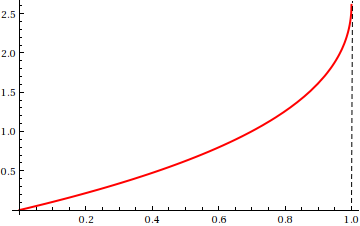
\includegraphics[width=300pt,keepaspectratio=true]{Addons/g32}
\caption{Plot della funzione $g_{3/2}(z)$ per $0\le z\le 1$.}

\end{figure}
\cleardoublepage
Possiamo scrivere la seconda delle equazioni del gas come:
\begin{equation}
\frac{\lambda^3}{v}-g_{3/2}(z)=\lambda^3\frac{\bra n_0\ket}{V}\;.
\end{equation}
Facciamo adesso un'importante osservazione. Per $T\to 0$ si ha $\lambda\to\infty$ mentre $z\to 1$. Se $\lambda^3/v>g_{3/2}(1)$, allora dovrà essere necessariamente, in virtù dell'equazione precedente, $\bra n_0\ket/V\ne 0$, cioè $\bra n_0\ket$ deve essere una quantità estensiva nel volume. Questo vuol dire che diminuendo sempre di più la temperatura il numero di particelle nello stato fondamentale diverge. \\
A $v$ fissato, il "punto di transizione" è dato da $\lambda_c^3=vg_{3/2}(1)$. Esiste quindi una temperatura critica data da:
\begin{equation}
kT_c=\frac{2\pi\hbar^2}{m(vg_{3/2}(1))^{2/3}}\;,
\end{equation}
sotto la quale le particelle condensano nello stato fondamentale. In altri termini, la BEC (\emph{Bose-Einstein Condensation}) avviene quando la lunghezza d'onda termica $\lambda$ è dell'ordine della distanza tipica tra le particelle $d=v^{1/3}$. \\
Possiamo leggere la condizione di criticità in termini del volume specifico: a $T$ fissata, esiste un volume critico:
\begin{equation}
v_c=\frac{\lambda^3}{g_{3/2}(1)}\;,
\end{equation}
sotto il quale avviene la BEC. Vogliamo adesso risolvere graficamente l'equazione:
\begin{equation}
\frac{\lambda^3}{v}=g_{3/2}(z)+\frac{\lambda^3}{V}\frac{z}{1-z}\;,
\end{equation}
in termini di $z$:

\begin{figure}[h]
\centering
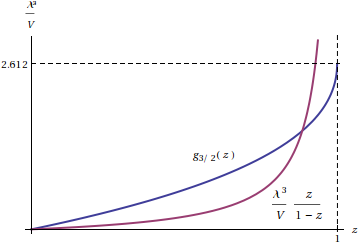
\includegraphics[width=300pt,keepaspectratio=true]{Addons/eq}
\caption{Grafico delle funzioni $g_{3/2}(z)$ e $\lambda^3 z/V(1-z)$.}
\end{figure}

La distanza tra la curva $\dfrac{\lambda^3}{V}\dfrac{z}{1-z}$ e l'asse $z=1$ è dell'ordine di $1/V$. La somma delle due funzioni ha un andamento del tipo:

\begin{figure}[h]
\centering
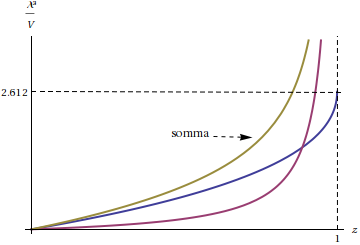
\includegraphics[width=300pt,keepaspectratio=true]{Addons/somma}
\caption{Somma delle funzioni $g_{3/2}(z)$ e $\lambda^3z/V(1-z)$.}
\end{figure}
\pagebreak

Nel limite termodinamico $V\to\infty$ si trova per $z$ l'espressione:
\begin{equation}
\begin{cases}
1\qquad \mbox{se}\; \dfrac{\lambda^3}{v}>2.612\qquad\Longleftrightarrow\qquad T<T_c\;, \\
\\
\mbox{soluzione di}\; g_{3/2}(z)=\dfrac{\lambda^3}{v}\qquad \mbox{se}\;\dfrac{\lambda^3}{v}<2.612\qquad \Longleftrightarrow \qquad T>T_c\;.
\end{cases}
\end{equation}
Calcoliamo adesso la frazione di condensato, ossia il valore di $\bra n_0\ket/N$:
\begin{equation}
\frac{\bra n_0\ket}{N}=\frac{\bra n_0\ket}{V}v=1-\frac{v}{\lambda^3}g_{3/2}(z)=\begin{cases}
0\qquad \mbox{per}\; T>T_c\;, \\
\\
1-\dfrac{v}{\lambda^3}g_{3/2}(1)\qquad\mbox{per}\; T>T_c\;.
\end{cases}
\end{equation}
Quindi al di sopra della temperatura critica, lo stato fondamentale non è macroscopicamente popolato. Per $T<T_c$ si ha:
\begin{equation}
\frac{\bra n_0\ket}{N}=1-\frac{v}{\lambda^3}g_{3/2}(1)=1-\frac{v}{v_c}=1-\left(\frac{T}{T_c}\right)^{3/2}\;.
\end{equation}
Quindi l'andamento dell'occupazione dello stato fondamentale è del tipo:

\begin{center}
\begingroup
  \makeatletter
  \providecommand\color[2][]{%
    \GenericError{(gnuplot) \space\space\space\@spaces}{%
      Package color not loaded in conjunction with
      terminal option `colourtext'%
    }{See the gnuplot documentation for explanation.%
    }{Either use 'blacktext' in gnuplot or load the package
      color.sty in LaTeX.}%
    \renewcommand\color[2][]{}%
  }%
  \providecommand\includegraphics[2][]{%
    \GenericError{(gnuplot) \space\space\space\@spaces}{%
      Package graphicx or graphics not loaded%
    }{See the gnuplot documentation for explanation.%
    }{The gnuplot epslatex terminal needs graphicx.sty or graphics.sty.}%
    \renewcommand\includegraphics[2][]{}%
  }%
  \providecommand\rotatebox[2]{#2}%
  \@ifundefined{ifGPcolor}{%
    \newif\ifGPcolor
    \GPcolorfalse
  }{}%
  \@ifundefined{ifGPblacktext}{%
    \newif\ifGPblacktext
    \GPblacktexttrue
  }{}%
  % define a \g@addto@macro without @ in the name:
  \let\gplgaddtomacro\g@addto@macro
  % define empty templates for all commands taking text:
  \gdef\gplbacktext{}%
  \gdef\gplfronttext{}%
  \makeatother
  \ifGPblacktext
    % no textcolor at all
    \def\colorrgb#1{}%
    \def\colorgray#1{}%
  \else
    % gray or color?
    \ifGPcolor
      \def\colorrgb#1{\color[rgb]{#1}}%
      \def\colorgray#1{\color[gray]{#1}}%
      \expandafter\def\csname LTw\endcsname{\color{white}}%
      \expandafter\def\csname LTb\endcsname{\color{black}}%
      \expandafter\def\csname LTa\endcsname{\color{black}}%
      \expandafter\def\csname LT0\endcsname{\color[rgb]{1,0,0}}%
      \expandafter\def\csname LT1\endcsname{\color[rgb]{0,1,0}}%
      \expandafter\def\csname LT2\endcsname{\color[rgb]{0,0,1}}%
      \expandafter\def\csname LT3\endcsname{\color[rgb]{1,0,1}}%
      \expandafter\def\csname LT4\endcsname{\color[rgb]{0,1,1}}%
      \expandafter\def\csname LT5\endcsname{\color[rgb]{1,1,0}}%
      \expandafter\def\csname LT6\endcsname{\color[rgb]{0,0,0}}%
      \expandafter\def\csname LT7\endcsname{\color[rgb]{1,0.3,0}}%
      \expandafter\def\csname LT8\endcsname{\color[rgb]{0.5,0.5,0.5}}%
    \else
      % gray
      \def\colorrgb#1{\color{black}}%
      \def\colorgray#1{\color[gray]{#1}}%
      \expandafter\def\csname LTw\endcsname{\color{white}}%
      \expandafter\def\csname LTb\endcsname{\color{black}}%
      \expandafter\def\csname LTa\endcsname{\color{black}}%
      \expandafter\def\csname LT0\endcsname{\color{black}}%
      \expandafter\def\csname LT1\endcsname{\color{black}}%
      \expandafter\def\csname LT2\endcsname{\color{black}}%
      \expandafter\def\csname LT3\endcsname{\color{black}}%
      \expandafter\def\csname LT4\endcsname{\color{black}}%
      \expandafter\def\csname LT5\endcsname{\color{black}}%
      \expandafter\def\csname LT6\endcsname{\color{black}}%
      \expandafter\def\csname LT7\endcsname{\color{black}}%
      \expandafter\def\csname LT8\endcsname{\color{black}}%
    \fi
  \fi
    \setlength{\unitlength}{0.0500bp}%
    \ifx\gptboxheight\undefined%
      \newlength{\gptboxheight}%
      \newlength{\gptboxwidth}%
      \newsavebox{\gptboxtext}%
    \fi%
    \setlength{\fboxrule}{0.5pt}%
    \setlength{\fboxsep}{1pt}%
\begin{picture}(7200.00,5040.00)%
    \gplgaddtomacro\gplbacktext{%
      \csname LTb\endcsname%
      \put(550,704){\makebox(0,0)[r]{\strut{}}}%
      \put(550,4379){\makebox(0,0)[r]{\strut{}}}%
      \put(550,2542){\makebox(0,0)[r]{\strut{}$1$}}%
      \put(6803,484){\makebox(0,0){\strut{}}}%
      \put(682,484){\makebox(0,0){\strut{}$0$}}%
      \put(3743,484){\makebox(0,0){\strut{}$1$}}%
    }%
    \gplgaddtomacro\gplfronttext{%
      \csname LTb\endcsname%
      \put(176,2541){\rotatebox{-270}{\makebox(0,0){\strut{}Condensate fraction $\bra n_0 \ket /N$}}}%
      \put(3742,154){\makebox(0,0){\strut{}Normalized temperature $T/T_c$}}%
      \put(3742,4709){\makebox(0,0){\strut{}Ground state occupation}}%
    }%
    \gplbacktext
    \put(0,0){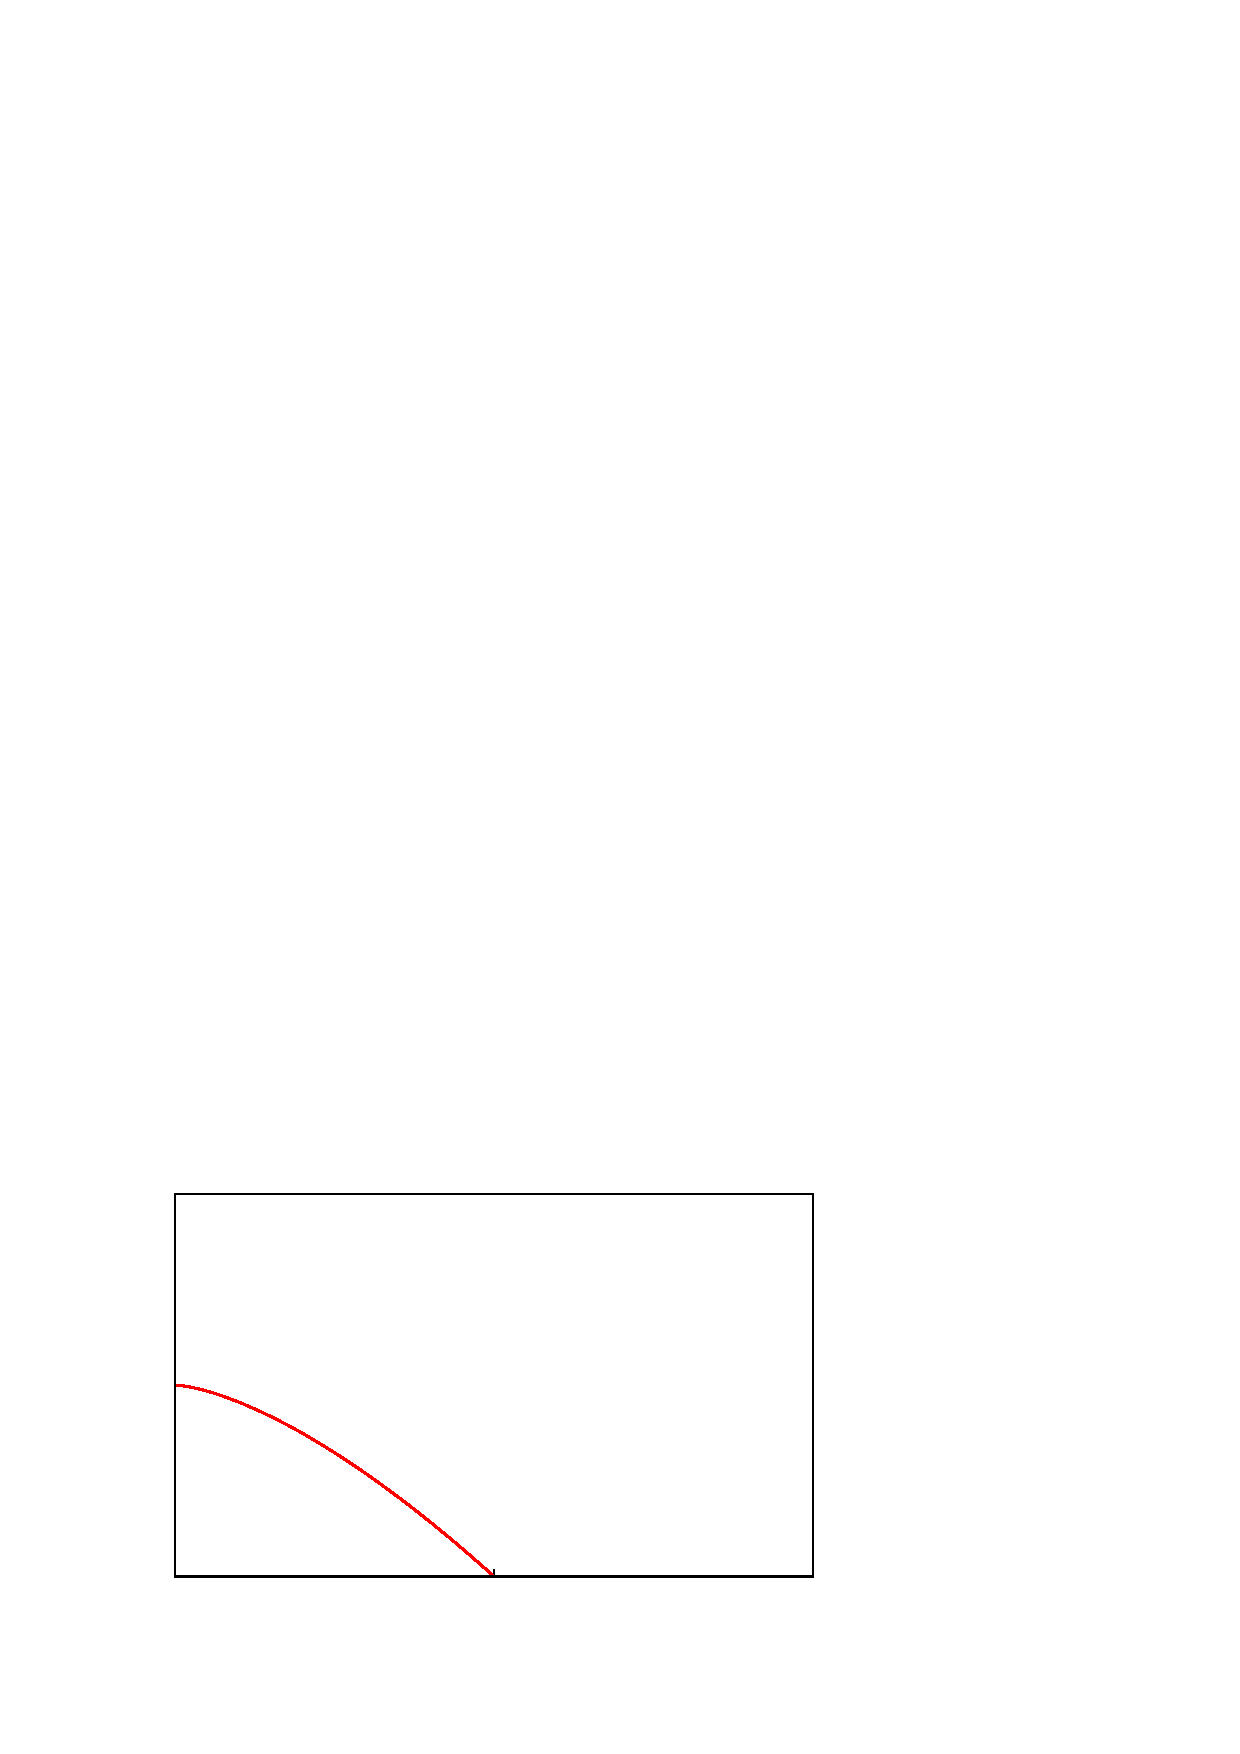
\includegraphics{Addons/condensatefraction}}%
    \gplfronttext
  \end{picture}%
\endgroup

\end{center}

Come sarebbero cambiate le cose se avessimo modificato l'equazione aggiungendo a mano anche la popolazione del primo stato eccitato, cioè:
$$
\frac{1}{v}=\frac{1}{\lambda^3}g_{3/2}(z)+\frac{\bra n_0\ket}{V}+\frac{\bra n_1\ket}{V}\;.
$$
Dalla definizione:
$$
\frac{\bra n_1\ket}{V}=\frac{1}{V}\frac{1}{z^{-1}e^{\beta\epsilon_1}-1}\le \frac{1}{V}\frac{1}{e^{\beta\epsilon_1}-1}\;,
$$
con (ricordando che siamo in una scatola di lato $L$ con condizioni periodiche):
\begin{align*}
\epsilon_1 &= \frac{p_1^2}{2m}\;, \\
\mathbf{p}&=\frac{2\pi\hbar\mathbf{n}}{L}=\frac{2\pi\hbar}{L}\hat{\mathbf{x}}\;,
\end{align*}
perché il primo stato eccitato ha $\mathbf{n}=(1,0,0)$ (tre volte degenere). Allora:
$$
\epsilon_1=\left(\frac{2\pi\hbar}{L}\right)^2\frac{1}{2m}=\frac{1}{2m}\frac{(2\pi\hbar)^2}{V^{2/3}}\;.
$$
Nel limite termodinamico, $\epsilon_1\to 0$, quindi:
$$
\frac{1}{V}\frac{1}{e^{\beta\epsilon_1}-1}\simeq \frac{1}{V}\frac{1}{\beta\epsilon_1}=\frac{1}{\beta V}\frac{2mV^{2/3}}{(2\pi\hbar)^2}\propto\frac{1}{V^{1/3}}\to 0\;.
$$
Quindi tutti gli stati eccitati, in regime di condensazione, non sono macroscopicamente popolati. \\
\\
L'equazione di stato per un gas di Bose ideale nel limite termodinamico assume la forma:
\begin{equation*}
\beta p=\frac{1}{\lambda^3}g_{5/2}(z)\;,
\end{equation*}
da cui:
\begin{equation}
\beta p=\begin{cases}
\dfrac{1}{\lambda^3}g_{5/2}(z)\qquad \mbox{per}\; T>T_c\;, \\
\\
\dfrac{1}{\lambda^3}g_{5/2}(1)\qquad \mbox{per}\; T<T_c\;.
\end{cases}
\end{equation}
Notiamo quindi che in regime di condensazione la pressione non dipende dal volume. Facendo un grafico nel piano $p-V$ si ottiene il seguente andamento:

\begin{figure}[h]
\centering
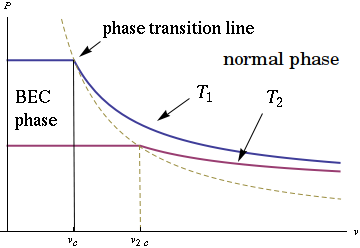
\includegraphics[width=300pt,keepaspectratio=true]{Addons/pressure}
\caption{\footnotesize{Caratteristica $p-v$ di un gas di Bose.}}
\end{figure}
\pagebreak

L'equazione dell'isoterma alla temperatura critica (linea di transizione) è data da:
$$
\beta p=\frac{1}{\lambda^3}g_{5/2}(1)\qquad\Longrightarrow\qquad p=\frac{2\pi\hbar^2}{m}\frac{1}{\lambda^5}g_{5/2}(1)\;.
$$
Alla transizione, $\lambda^3/V=g_{3/2}(1)$, da cui ricaviamo il valore di $\lambda$ che sostituiamo nella relazione precedente per ottenere l'equazione della linea di transizione:
\begin{equation}
pv^{5/3}=\frac{2\pi\hbar^2}{m}\frac{g_{5/2}(1)}{[g_{3/2}(1)]^{5/3}}\;.
\end{equation}
Nella fase di condensazione abbiamo compresenza tra condensato e gas e variando la pressione non varia il volume, bensì viene favorito il passaggio da una fase all'altra. Definiamo la \emph{tensione di vapore} $p_0$ come la pressione sulla linea costante. Per un condensato:
\begin{equation}
p_0=\frac{kT}{\lambda^3}g_{5/2}(1)\;.
\end{equation}
Si ha:
\begin{align*}
\dev{p_0}{T} &= g_{5/2}(1)\left[\frac{k}{\lambda^3}-kT\frac{\diff{\lambda^3}}{\diff{T}}\frac{1}{\lambda^6}\right] \\
&= g_{5/2}(1)\left[\frac{k}{\lambda^3}+\left(\frac{2\pi\hbar}{mk}\right)^{3/2}\frac{3}{2}T^{-5/2}\frac{1}{\lambda^6}\right] \\
&= g_{5/2}(1)\left[\frac{k}{\lambda^3}+kT\frac{3}{2}\frac{\lambda^3}{T}\frac{1}{\lambda^6}\right] \\
&= g_{5/2}(1)\left[\frac{k}{\lambda^3}+\frac{3}{2}\frac{k}{\lambda^3}\right]=\frac{5}{2}\frac{kg_{5/2}(1)}{\lambda^3}\\
&=\frac{1}{Tv_c}\left[\frac{5}{2}kT\frac{g_{5/2}(1)}{g_{3/2}(1)}\right]\;,
\end{align*}
dove abbiamo usato la condizione di criticità $v_c=\lambda^3/g_{3/2}(1)$. Riconosciamo quindi la forma dell'equazione di Clapeyron:
\begin{equation}
\dev{p_0}{T}=\frac{1}{T\delta v}L\;,
\end{equation}
dove $\Delta v$ è la differenza di volume tra la fase liquida e quella di vapore e $L$ è il calore latente. Per un condensato, $\Delta v=v_c$ e per il calore latente si ottiene l'espressione:
\begin{equation}
L=\frac{5}{2}kT\frac{g_{5/2}(1)}{g_{3/2}(1)}\;.
\end{equation}
L'esistenza di un calore latente ci dice che la transizione di fase gas-condensato è del primo ordine (vero solo per bosoni non interagenti).
\section{Quantità termodinamiche di un condensato}
L'espressione dell'energia per particella di un condensato è data da:
\begin{equation}
\frac{E}{N}=\frac{3}{2}pv=\begin{cases}
\dfrac{3}{2}\dfrac{kTv}{\lambda^3}g_{5/2}(z)\qquad T>T_c\;, \\
\\
\dfrac{3}{2}\dfrac{kTv}{\lambda^3}g_{5/2}(1)\qquad T<T_c\;,
\end{cases}
\end{equation}
mentre quella dell'entropia è:
\begin{equation}
\frac{S}{Nk}=\begin{cases}
\dfrac{5}{2}\dfrac{v}{\lambda^3}g_{5/2}(z)-\ln z\qquad T>T_c\;, \\
\\
\dfrac{5}{2}\dfrac{v}{\lambda^3}g_{5/2}(1)\qquad T<T_c\;.
\end{cases}
\end{equation}
Notiamo che, per basse temperature, $S/(Nk)\propto T^{3/2}$, e quindi tende a zero in accordo con il terzo principio. Un'altra importante osservazione è che la fase condensata non ha entropia, ossia per $T<T_c$ l'entropia è dovuta unicamente al contributo della \emph{frazione gassosa}, definita dal rapporto tra il numero di particelle negli stati eccitati $N_{\mathrm{ex}}$ e il numero di particelle totali:
\begin{equation}
\frac{N_{\mathrm{ex}}}{N}=\left(\frac{T}{T_c}\right)^{3/2}=\frac{v}{v_c}\;.
\end{equation}
Allora l'entropia si può scrivere in regime di condensazione come:
\begin{equation}
\frac{S}{Nk}=\left(\frac{T}{T_c}\right)^{3/2}s\;,
\end{equation}
dove $s$ è la densità di entropia del gas, data da:
\begin{equation}
s=\frac{5}{2}k\frac{g_{5/2}(1)}{g_{3/2}(1)}\;,
\end{equation}
confrontando con l'espressione del calore latente si ottiene la relazione $L=sT$. \\
Il calore specifico infine è dato da:
\begin{equation}
\frac{C_v}{Nk}=\begin{cases}
\dfrac{15}{4}\dfrac{v}{\lambda^3}g_{5/2}(z)-\dfrac{9}{4}\dfrac{g_{3/2}(z)}{g_{1/2}(z)}\qquad T>T_c \;,\\
\\
\dfrac{15}{4}\dfrac{v}{\lambda^3}g_{5/2}(1)\qquad T<T_c\;.
\end{cases}
\end{equation}
L'andamento del calore specifico è il seguente:
\begin{figure}[h]
\centering
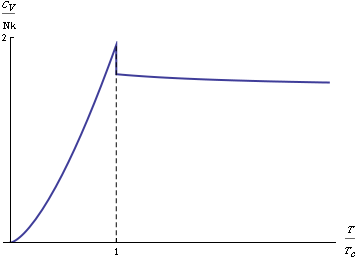
\includegraphics[width=300pt,keepaspectratio=true]{Addons/lambdatransition}
\caption{Andamento di $C_v/Nk$ e transizione $\lambda$.}
\end{figure}
\pagebreak

Il calore specifico presenta una discontinuità nella derivata prima alla temperatura critica che, per la forma dell'andamento, prende il nome di transizione $\lambda$.

\section{Gas ideale di Bose in dimensione arbitraria}
Per un gas di Bose generico, valgono, indipendententemente dalla dimensione, le due equazioni:
\begin{align*}
\beta pV&=\ln\zpart(z,V,T)=-\sum_{\mathbf{p}}\ln(1-ze^{-\beta \epsilon_{\mathbf{p}}})\;, \\
N&=z\frac{\partial}{\partial z}\ln\zpart(z,V,T)=\sum_{\mathbf{p}}\frac{1}{z^{-1}e^{\beta\epsilon_{\mathbf{p}}}-1}\;.
\end{align*}
Per un gas ideale si ha:
$$
\epsilon_{\mathbf{p}}=\frac{|\mathbf{p}|^2}{2m},\qquad \mathbf{p}=\frac{2\pi\hbar}{L}\mathbf{n}\;.
$$
L'unica differenze è che in $d$ dimensioni si ha $\mathbf{n}=(n_1,n_2,\ldots,n_d)$. Allora il limite termodinamico si esplicita tramite la sostituzione:
$$
\sum_{\mathbf{p}} \longrightarrow \frac{S_d}{(2\pi\hbar)^d}V\int\diff{p}\;p^{d-1}\;,
$$
dove $S_d$ è la superficie della sfera $d$-dimensionale di raggio unitario, data da:
\begin{equation}
S_d=\frac{2\pi^{d/2}}{\Gamma(d/2)}=\begin{cases}
4\pi\qquad d=3\;, \\
\\
2\pi \qquad d=2\;, \\
\\
2\qquad d=1\;.
\end{cases}
\end{equation}
Eseguendo dunque il limite si ottiene:
\begin{align}
\beta p &=-\frac{2\pi^{d/2}}{\Gamma(d/2)}\frac{1}{(2\pi\hbar)^d}\int\diff{p}\;p^{d-1}\ln(1-ze^{-\beta p^2/2m})-\frac{1}{V}\ln(1-z)\;, \notag \\
N &= \frac{2\pi^{d/2}}{\Gamma(d/2)}\frac{V}{(2\pi\hbar)^d}\int\diff{p}\;p^{d-1}\frac{1}{z^{-1}e^{\beta p^2/2m}-1}+\frac{z}{1-z}\;.
\end{align}
Concentriamoci sulla seconda equazione ed effettuiamo la sostituzione:
\begin{align*}
\frac{\beta p^2}{2m}&= x\;, \\
p&=\sqrt{\frac{2mx}{\beta}}\;, \\
\frac{\beta p\diff{p}}{m}&=\diff{x}\; \Longrightarrow\; p^{d-1}\diff{p}=p^{d-2}p\diff{p}=\left(\frac{2mx}{\beta}\right)^{\frac{d-2}{2}}\frac{m}{\beta}\diff{x}\;,
\end{align*}
ottenendo:
$$
\frac{N}{V}=\frac{2\pi^{d/2}}{\Gamma(d/2)}\frac{1}{(2\pi\hbar)^d}\left(\frac{2m}{\beta}\right)^{(d-2)/2}\frac{m}{\beta}\int\diff{x}\;\frac{x^{d/2-1}}{z^{-1}e^x-1}+\frac{1}{V}\frac{z}{1-z}\;.
$$
Ricordando che $\lambda=\sqrt{2\pi\hbar^2\beta/m}$, il prefattore diventa:
$$
\frac{\pi^{d/2}}{(2\pi\hbar)^d}\left(\frac{2m}{\beta})^{d/2}\right)=\left(\frac{m}{2\pi\hbar^2\beta}\right)^{d/2}=\frac{1}{\lambda^d}\;,
$$
e dunque:
$$
\frac{N}{V}=\frac{1}{\lambda^d}\frac{1}{\Gamma(d/2)}\int_0^{+\infty}\diff{x}\;\frac{x^{d/2-1}}{z^{-1}e^x-1}+\frac{1}{V}\frac{z}{1-z}\;.
$$
Definiamo, in analogia con il caso tridimensionale:
\begin{align}
g_{\nu}(z) &= \frac{1}{\Gamma(\nu)}\int_0^{+\infty}\diff{x}\;\frac{x^{\nu-1}}{z^{-1}e^x-1} \\
&= \frac{1}{\Gamma(\nu)}\int_0^{+\infty}\diff{x}\;x^{\nu-1}\sum_{\ell=1}^{\infty}(ze^{-x})^{\ell} \notag \\
&= \sum_{\ell=1}^{\infty}z^{\ell}\frac{1}{\Gamma(\nu)}\int_0^{+\infty}\diff{x}\;x^{\nu-1}e^{-\ell x} \qquad (y=\ell x) \notag \\
&=\sum_{\ell=1}^{\infty}\frac{z^{\ell}}{\ell^{\nu}}\frac{1}{\Gamma(\nu)}\underbrace{\int_0^{+\infty}\diff{y}\;y^{\nu-1}e^{-y}}_{=\Gamma(\nu)} \notag \\
&= \sum_{\ell=1}^{\infty}\frac{z^{\ell}}{\ell^{\nu}}\;.
\end{align}
Per $z\to 1$ si ha:
\begin{equation}
g_{\nu}(1)=\sum_{\ell=1}^{\infty}\frac{1}{\ell^{\nu}}=\begin{cases}
\zeta(\nu)\qquad \nu>1\;, \\
\\
\infty \qquad \nu\le 1\;.
\end{cases}
\end{equation}
In particolare, per $\nu=1$ $g_1(z)=\sum_{\ell=1}^{\infty}z^{\ell}/\ell=-\ln(1-z)$. Vale inoltre la seguente relazione ricorsiva:
\begin{equation}
z\frac{\partial}{\partial z}g_{\nu}(z)=g_{\nu-1}(z)\;.
\end{equation}
Infine:
\begin{equation}
\frac{N}{V}=\frac{1}{v}=\frac{g_{d/2}(z)}{\lambda^d}+\frac{1}{V}\frac{z}{1-z}=\frac{g_{d/2}(z)}{\lambda^d}+\frac{\bra n_0\ket}{V}\;.
\end{equation}
L'andamento della funzione per $d=1,2,3,4$ è visibile nel seguente grafico:

\begin{figure}[h]
\centering
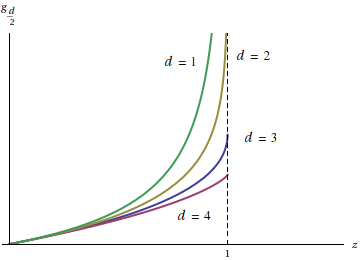
\includegraphics[width=300pt,keepaspectratio=true]{Addons/bosefunctions}
\caption{\footnotesize{Andamento di $g_{d/2}(z)$ per $d=1,2,3,4$.}}
\end{figure}
\pagebreak
L'equazione che determina $z$ è:
\begin{equation}
\frac{\lambda^d}{v}-g_{d/2}(z)=\lambda^d\frac{\bra n_0\ket}{V}\;.
\end{equation}
Per $d\le 2$, tuttavia, $g_{d/2}(z)$ non è più limitata, quindi non è più valida l'argomentazione che abbiamo precedentemente usato per $d=3$. Concludiamo che per sistemi unidimensionali e bidimensionali non si può verificare il fenomeno della BEC, mentre per sistemi di dimensione $d>2$ essa può avvenire. Ponendo $\lambda^d/v=g_{d/2}(1)$ definiamo:
\begin{equation}
v_c=\frac{\lambda^d}{g_{d/2}(1)}\qquad kT_c=\frac{2\pi\hbar^2}{m(vg_{d/2}(1))^{2/d}}\;,
\end{equation}
e la soluzione per $z$ è:
\begin{equation}
z=\begin{cases}
1\qquad \mbox{se}\; \dfrac{\lambda^d}{v}>g_{d/2}(1)\qquad \mbox{(questa parte non esiste per}\; d=1,2)\;, \\
\\
\mbox{soluzione di}\; g_{d/2}(z)=\dfrac{\lambda^d}{v}\qquad \mbox{se}\; \dfrac{\lambda^d}{v}<g_{d/2}(1)\;.
\end{cases}
\end{equation}
La frazione di condensato sarà quindi:
\begin{equation}
\frac{\bra n_0\ket}{N}=\frac{\bra n_0\ket}{V}\frac{V}{N}=1-g_{d/2}(z)\frac{v}{\lambda^d}=\begin{cases}
0\qquad \mbox{per}\; T>T_c\;, \\
\\
1-\left(\dfrac{T}{T_c}\right)^{d/2}\qquad \mbox{per}\; T<T_c\;.
\end{cases}
\end{equation}
La Termodinamica segue da:
$$
\beta pV=\frac{1}{\lambda^{d/2}}g_{d/2+1}(z)+\underbrace{\frac{1}{V}\ln(1-z)}_{\to 0}\;.
$$
L'unica osservazione che facciamo è che $C_v,S\propto T^{d/2}$ per piccole temperature, e quindi vanno a zero con $T$ in accordo con il terzo principio.
\section{Limite di alta temperatura per $d=3$}
Per alte temperature $\lambda^3/v=g_{3/2}(z)\ll 1$ e quindi anche $z\ll 1$. Possiamo sviluppare quindi $g_{3/2}(z)$ ritenendo solo i termini fino al secondo ordine:
\begin{equation}
\frac{\lambda^3}{v}\simeq z+\frac{z^2}{2^{3/2}}+o(z^3)\;. \label{ch3_zetasviluppo}
\end{equation}
Quindi, al primo ordine:
\begin{equation}
z=\frac{\lambda^3}{v}+o\left(\left(\frac{\lambda^3}{v}\right)^2\right)\;.
\end{equation}
Al secondo ordine possiamo scrivere:
$$
z=\frac{\lambda^3}{v}+b\left(\frac{\lambda^3}{v}\right)^2\;,
$$
sostituendo questa in \eqref{ch3_zetasviluppo} e ritenendo fino al secondo ordine, ricaviamo per $b$ il valore $b=-2^{-3/2}$. Quindi, al secondo ordine, si ha:
\begin{equation}
z=\frac{\lambda^3}{v}-\frac{1}{2^{3/2}}\left(\frac{\lambda^3}{v}\right)^2+o\left(\left(\frac{\lambda^3}{v}\right)^3\right)\;.
\end{equation}
L'equazione di stato è quindi data da:
\begin{align}
\beta pv &=\frac{v}{\lambda^3}g_{5/2}(z)=\frac{v}{\lambda^3}\left(z+\frac{z^2}{2^{5/2}}+\cdots\right) \notag \\
&=\frac{v}{\lambda^3}\left[\frac{\lambda^3}{v}-\left(\frac{\lambda^3}{v}\right)^2\frac{1}{2^{3/2}}+\left(\frac{\lambda^3}{v}\right)^2\frac{1}{2^{5/2}}+\cdots\right] \notag \\
&= 1-\frac{\lambda^3}{v}\frac{1}{2^{5/2}}\;,
\end{align}
dove il primo termine è proprio l'equazione di stato di un gas perfetto classico e il secondo termine rappresenta le correzioni quantistiche.
\section{BEC in una trappola armonica}
Consideriamo un potenziale armonico esterno che, fissata un'energia, confini gli atomi entro una certa regione:
\begin{figure}[h]
\centering
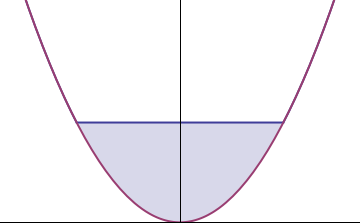
\includegraphics[width=300pt,keepaspectratio=true]{Addons/potentialwell}
\caption{\footnotesize{Trappola armonica.}}
\end{figure}
\pagebreak

L'Hamiltoniana a cui sono sottoposti gli atomi è quella di un oscillatore armonico tridimensionale:
\begin{equation}
H=\sum_{i=1}^N\left[\frac{\mathbf{p}_i^2}{2m}+\frac{1}{2}m\omega^2\mathbf{r}_i^2\right]\;.
\end{equation}
Sappiamo che gli autostati possono essere classificati tramite tre numeri quantici $\ell_1,\ell_2,\ell_3$:
$$
\epsilon_{\ell_a,\ell_b,\ell_c}=\hbar\omega\left(\ell_1+\ell_2+\ell_3+\frac{3}{2}\right),\qquad \ell_i=0,1,\ldots,\infty\;.
$$
Essendo i livelli degeneri, possiamo riscrivere tutto in termini di un unico numero quantico $\ell=\ell_1+\ell_2+\ell_3$:
\begin{equation}
\epsilon_{\ell}=\hbar\omega\left(\ell+\frac{3}{2}\right),\qquad \ell=0,1,\ldots,\infty\;,
\end{equation}
con degenerazione $g_{\ell}=\dfrac{(\ell+1)(\ell+2)}{2}$. Adesso ricaviamo la statistica del sistema scrivendo il logaritmo della funzione di granpartizione:
\begin{equation}
\ln\zpart=-\sum_n\ln(1-ze^{-\beta\epsilon_n})=-\sum_{\ell=0}^{\infty}\frac{(\ell+1)(\ell+2)}{2}\ln(1-e^{-\beta\hbar\omega(\ell+3/2)})\;.
\end{equation}
Nel limite termodinamico, sostituiamo la serie con un integrale e trascuriamo i vari termini addizionali costanti perché di ordine superiore. Otteniamo perciò:
\begin{align}
\ln\zpart &= -\frac{1}{2}\int x^2\ln\left(1-ze^{-\beta\hbar\omega x}\right)\diff{x}\qquad\qquad\qquad \beta\hbar\omega x=y \notag \\
&= -\frac{1}{2}\frac{1}{(\beta\hbar\omega)^3}\int_0^{\infty}\diff{y}\; y^2\ln(1-ze^{-y}) \notag \\
&= \frac{1}{2}\left(\frac{kT}{\hbar\omega}\right)^3\sum_{n=1}^{\infty}\int_0^{\infty}\diff{y}\;y^2\frac{(ze^{-y})^n}{n} \notag \\
&= \left(\frac{kT}{\hbar\omega}\right)^3\sum_{n=1}^{\infty}\frac{z^n}{n}\frac{1}{2}\int_0^{\infty}\diff{y}\; y^2 e^{-ny} \qquad\qquad\qquad ny=t \notag \\
&=\left(\frac{kT}{\hbar\omega}\right)^3\sum_{n=1}^{\infty}\frac{z^n}{n^4}\frac{1}{2}\underbrace{\int_0^{\infty}\diff{t}\; t^2e^{-t}}_{=\Gamma(2)=2} \notag \\
&=\left(\frac{kT}{\hbar\omega}\right)^3\sum_{n=1}^{\infty}\frac{z^n}{n^4}\equiv \left(\frac{kT}{\hbar\omega}\right)^3 g_4(z)\;.
\end{align}
Da questa possiamo ricavare il numero di particelle $N$:
\begin{equation}
N=z\frac{\partial}{\partial z}\ln(1-z)+\frac{z}{1-z}=\left(\frac{kT}{\hbar\omega}\right)^3 z\frac{\partial}{\partial z}g_4(z)+\bra n_0\ket=\left(\frac{kT}{\hbar\omega}\right)^3g_3(z)+\bra n_0\ket\;.
\end{equation}
Dato che $g_3(1)=\zeta(3)\simeq 1.202$, concludiamo che nel sistema può verificarsi la BEC a condizione che
\begin{equation}
N-\left(\frac{kT}{\hbar\omega}\right)^3\zeta(3)\ge 0 \qquad \Longrightarrow\qquad \bra n_0\ket\ne 0, z=1\;.
\end{equation}
L'uguaglianza nella relazione precedente definisce la temperatura critica:
\begin{equation}
\frac{kT_c}{\hbar\omega}=\left(\frac{N}{\zeta(3)}\right)^{1/3}\;.
\end{equation}
Se inseriamo i numeri del primo esperimento del 1995 $N=2\cdot 10^4$ atomi intrappolati e laser di frequenza $\omega=100$ Hz, si trova:
$$
\frac{kT_c}{\hbar\omega}\simeq 25\qquad\Longrightarrow\qquad T_c\simeq 100\;\mathrm{nK}\;.
$$
Le frazioni di gas e di condensato sono rispettivamente:
\begin{align*}
\frac{N_{\mathrm{ex}}}{N}&=\frac{\zeta(3)}{N}\left(\frac{kT}{\hbar\omega}\right)^3=\left(\frac{T}{T_c}\right)^3\;, \\
\frac{\bra n_0\ket}{N} &= 1-\left(\frac{T}{T_c}\right)^3\;.
\end{align*}
Osserviamo che per eseguire il limite termodinamico in questo caso bisogna fare i limiti $N\to\infty,\omega\to 0$ con $N\omega^3=$ costante (distanza interatomica fissata). \\
Trattiamo adesso il caso bidimensionale. Per realizzare un sistema bidimensionale, è sufficiente realizzarne uno tridimensionale in cui in una delle direzioni si abbia $\omega$ molto grande, così che la parabola sia molto strizzata e complessivamente il sistema non veda per niente quella direzione. Calcoli del tutto identici a quelli precedenti portano a scrivere il logaritmo della funzione di granpartizione come:
\begin{equation}
\ln \zpart=\left(\frac{kT}{\hbar\omega}\right)^2g_3(z)\;,
\end{equation}
e per il numero di particelle:
\begin{equation}
N=\left(\frac{kT}{\hbar\omega}\right)^2g_2(z)+\bra n_0\ket\;,
\end{equation}
con $g_2(1)=\zeta(1)=\pi^2/6$. Quindi, anche in questo sistema può essere realizzata la BEC (mentre con condizioni periodiche non era possibile). \\
In una dimensione invece otteniamo nell'espressione di $N$ un $g_1(z)$, che diverge in $z=1$, e questo implica che in una trappola armonica unidimensionale non può avvenire la condensazione.
\chapter{Applicazioni della statistica di Fermi}
\section{Gas di Fermi ideale in tre dimensioni}
Le equazioni che descrivono un gas di Fermi ideale sono:
\begin{equation}
\begin{cases}
\beta p=\dfrac{f_{5/2}(z)}{\lambda^3}\;, \\
\\
\dfrac{1}{v}=\dfrac{f_{3/2}(z)}{\lambda^3}\;,
\end{cases},\qquad f_n(z)=\sum_{\ell=1}^{\infty}(-1)^{\ell+1}\frac{z^{\ell}}{\ell^n}\;,
\end{equation}
con:
$$
f_{3/2}(z)=\frac{4}{\sqrt{\pi}}\int_0^{\infty}\diff{x}\;\frac{x^2}{z^{-1}e^x+1}\;.
$$
Le funzioni $f_n(z)$ sono definite per ogni $z\in\mathbb{R}^+$. $f_{3/2}(z)$ è una funzione monotona crescente e positiva. Studiamone i limiti di alta e bassa temperatura. \\
Per $z\ll 1$, ossia nel limite di alta temperatura $\lambda^3/v\ll 1$, si può approssimare:
$$
f_{3/2}(z)\simeq z-\frac{z^2}{2^{3/2}}-\frac{z^2}{3^{3/2}}+o(z^3)\;,
$$
da cui:
$$
\frac{\lambda^3}{v}=z-\frac{z^2}{2^{3/2}}\qquad \Longrightarrow\qquad z=\frac{\lambda^3}{v}+\frac{1}{2^{3/2}}\left(\frac{\lambda^3}{v}\right)^2\;.
$$
Inoltre in questo limite si ha:
\begin{equation}
\bra n_{\mathbf{p}}\ket=\frac{ze^{-\beta\epsilon_{\mathbf{p}}}}{1\mp ze^{-\beta\epsilon_{\mathbf{p}}}}\simeq \frac{\lambda^3}{v}e^{-\beta\epsilon_{\mathbf{p}}}\;,
\end{equation}
che è proprio la distribuzione classica di Maxwell-Boltzmann (vale sia per bosoni che per fermioni). Per quanto riguarda l'equazione di stato si ottiene:
\begin{equation}
\beta p v=\frac{v}{\lambda^3}\left(z-\frac{z^2}{2^{5/2}}\right)=\frac{v}{\lambda^3}\left(\frac{\lambda^3}{v}+\frac{1}{2^{3/2}}\left(\frac{\lambda^3}{v}\right)^2-\frac{1}{2^{5/2}}\left(\frac{\lambda^3}{v}\right)^2\right)=1+\frac{1}{2^{5/2}}\frac{\lambda^3}{v}\;.
\end{equation}
Nel limite di bassa temperatura $\lambda^3/v\gg 1$, si utilizza il cosiddetto \emph{metodo di Sommerfeld}: si pone $z=e^{\nu}$, $\nu=\ln z=\mu/kT$ e si riscrive la funzione $f_{3/2}(z)$ come:
\begin{align*}
f_{3/2}(z) &= \frac{4}{\sqrt{\pi}}\int_0^{\infty}\diff{x}\;\frac{x^2}{e^{x^2-\nu}+1}\qquad \qquad x^2=y \\
&=\frac{2}{\sqrt{\pi}}\int_0^{\infty}\frac{y^{1/2}}{e^{y-\nu}+1}\diff{y} \qquad \qquad \mbox{integriamo per parti} \\
&= \frac{2}{\sqrt{\pi}}\frac{2}{3}\int_0^{\infty}\diff{y}\; \frac{y^{3/2}e^{y-\nu}}{(e^{y-\nu}+1)^2}\;.
\end{align*}
Adesso sviluppiamo $y^{3/2}$ intorno a $\nu$:
\begin{equation}
y^{3/2}=\nu^{3/2}+\frac{3}{2}\nu^{1/2}(y-\nu)+\frac{3}{8}\nu^{-1/2}(y-\nu)^2+\cdots\;.
\end{equation}
Sostituendo nell'integrale si ottiene:
\begin{align*}
f_{3/2}(z)&=\frac{4}{3\sqrt{\pi}}\int_0^{\infty}\diff{y}\;\frac{e^{y-\nu}}{(e^{y-\nu}+1)^2}\left[\nu^{3/2}+\frac{3}{2}\nu^{1/2}(y-\nu)+\frac{3}{8}\nu^{-1/2}(y-\nu)^2+\cdots\right] \\
&=\frac{4}{3\sqrt{\pi}}\int_{-\nu}^{\infty}\diff{t}\;\frac{e^t}{(e^t+1)^2}\left[\nu^{3/2}+\frac{3}{2}\nu^{1/2}t+\frac{3}{8}\nu^{-1/2}t^2+\cdots\right]\;.
\end{align*}
Adesso, notiamo che $\int_{-\nu}^{+\infty}=\int_{-\infty}^{+\infty}-\int_{-\infty}^{-\nu}$ e, nel limite $z\gg 1$, cioè $\nu\gg 1$, si ha $\int_{-\infty}^{-\nu}=o(e^{-\nu})$, quindi:
\begin{align*}
f_{3/2}(z) &= \frac{4}{3\sqrt{\pi}}\int_{-\infty}^{+\infty}\diff{t}\; \frac{e^t}{(e^t+1)^2}\left[\nu^{3/2}+\frac{3}{2}\nu^{1/2}t+\frac{3}{8}\nu^{-1/2}t^2+\cdots\right]+o(e^{-\nu}) \\
&= \frac{4}{3\sqrt{\pi}}\left[ I_0\nu^{3/2}+\frac{3}{2}I_1\nu^{1/2}+\frac{3}{8}I_2\nu^{-1/2}+\cdots\right]+o(e^{-\nu})\;,
\end{align*}
dove:
\begin{equation}
I_n=\int_{-\infty}^{+\infty}\diff{t}\; \frac{t^ne^t}{(e^t+1)^2}\;. \label{ch4_infermioni}
\end{equation}
Per $n$ dispari, l'integrando in \eqref{ch4_infermioni} è dispari, quindi $I_{2n+1}\equiv 0$. Si ha inoltre $I_0=1,I_1=\pi^2/3$ e, in generale, per $n$ pari, $I_n=(n-1)!(2n)(1-2^{2n})\zeta(n)$. In conclusione:
\begin{align}
f_{3/2}(z)&=\frac{4}{3\sqrt{\pi}}\left[(\ln z)^{3/2}+\frac{\pi^2}{8}(\ln z)^{-1/2}+\cdots\right]+o(1/z) \notag \\
&= \frac{4}{3\sqrt{\pi}}(\ln z)^{3/2}\left[1+\frac{\pi^2}{8}(\ln z)^{-2}+o((\ln z)^{-4})\right]\;. \label{ch4_sviluppof32}
\end{align}
Un'analoga procedura porta all'espressione per $f_{5/2}(z)$:
\begin{equation}
f_{5/2}(z)=\frac{8}{15\sqrt{\pi}}(\ln z)^{5/2}\left[1+\frac{5\pi^2}{8(\ln z)^2}+o((\ln z)^{-4})\right]\;.
\end{equation}
L'energia interna di un gas ideale di Fermi è data da:
\begin{equation}
E=-\frac{\partial}{\partial\beta}\ln\zpart(z,V,T)=\frac{3}{2}\frac{kT}{\lambda^3}f_{5/2}(z)=\frac{3}{2}pV\;. \label{ch4_enintfermi}
\end{equation}
Questa espressione è valida per tutte le temperature e per ogni valore di $z$. Risolviamo adesso l'equazione:
$$
\frac{\lambda^3}{v}=f_{3/2}(z)\;,
$$
nel limite $z\gg 1$. Inserendo lo sviluppo \eqref{ch4_sviluppof32} al primo ordine troviamo:
\begin{equation}
\frac{\lambda^3}{v}=\frac{4}{3\sqrt{\pi}}(\ln z)^{3/2}\;.
\end{equation}
Poniamo $z=e^{\beta\epsilon_F}$, dove $\epsilon_F$ è l'\emph{energia di Fermi}. Risolvendo per $\epsilon_F$ si trova:
\begin{align}
\left(\frac{2\pi\hbar^2}{mkT}\right)^{3/2}\frac{1}{v}&=\frac{4}{3\sqrt{\pi}}(\beta\epsilon_F)^{3/2} \notag\;, \\
\epsilon_F &= \frac{\hbar^2}{2m}\left(\frac{6\pi^2}{v}\right)^{2/3}\;.
\end{align}
Riprendendo la definizione della distribuzione di Fermi:
$$
\bra n_{\mathbf{p}}\ket =\frac{1}{e^{\beta(\epsilon_{\mathbf{p}}-\epsilon_F)}+1}\;,
$$
per $T\to 0$, cioè $\beta\to\infty$ si ha:
\begin{equation}
\bra n_p\ket \longrightarrow \begin{cases}
0\qquad \mbox{se}\; \epsilon_{\mathbf{p}}>\epsilon_F\;, \\
\\
1\qquad \mbox{se}\; \epsilon_{\mathbf{p}}\le \epsilon_F\;,
\end{cases}\equiv \theta(\epsilon_F-\epsilon_{\mathbf{p}})\;.
\end{equation}

\begin{center}
\setlength{\unitlength}{0.240900pt}
\ifx\plotpoint\undefined\newsavebox{\plotpoint}\fi
\sbox{\plotpoint}{\rule[-0.200pt]{0.400pt}{0.400pt}}%
\begin{picture}(1500,900)(0,0)
\sbox{\plotpoint}{\rule[-0.200pt]{0.400pt}{0.400pt}}%
\put(111.0,131.0){\rule[-0.200pt]{4.818pt}{0.400pt}}
\put(111.0,131.0){\rule[-0.200pt]{4.818pt}{0.400pt}}
\put(91,561){\makebox(0,0)[r]{$1$}}
\put(111.0,561.0){\rule[-0.200pt]{4.818pt}{0.400pt}}
\put(775,90){\makebox(0,0){$\epsilon_F$}}
\put(775.0,131.0){\rule[-0.200pt]{0.400pt}{4.818pt}}
\put(1439.0,131.0){\rule[-0.200pt]{0.400pt}{4.818pt}}
\put(111,90){\makebox(0,0){$0$}}
\put(111.0,131.0){\rule[-0.200pt]{0.400pt}{4.818pt}}
\put(775.0,131.0){\rule[-0.200pt]{0.400pt}{4.818pt}}
\put(1439.0,131.0){\rule[-0.200pt]{0.400pt}{4.818pt}}
\put(111.0,131.0){\rule[-0.200pt]{0.400pt}{155.380pt}}
\put(111.0,131.0){\rule[-0.200pt]{319.915pt}{0.400pt}}
\put(1439.0,131.0){\rule[-0.200pt]{0.400pt}{155.380pt}}
\put(111.0,776.0){\rule[-0.200pt]{319.915pt}{0.400pt}}
\put(30,453){\makebox(0,0){\rotatebox{90}{Mean occupation $\bra n_p\ket$}}}
\put(775,29){\makebox(0,0){Energy of the level $\epsilon_p$}}
\put(775,838){\makebox(0,0){Fermi distribution at $T=0$}}
\put(111,561){\usebox{\plotpoint}}
\multiput(768.58,509.59)(0.494,-15.774){25}{\rule{0.119pt}{12.386pt}}
\multiput(767.17,535.29)(14.000,-404.293){2}{\rule{0.400pt}{6.193pt}}
\put(111.0,561.0){\rule[-0.200pt]{158.271pt}{0.400pt}}
\put(782.0,131.0){\rule[-0.200pt]{158.271pt}{0.400pt}}
\put(111.0,131.0){\rule[-0.200pt]{0.400pt}{155.380pt}}
\put(111.0,131.0){\rule[-0.200pt]{319.915pt}{0.400pt}}
\put(1439.0,131.0){\rule[-0.200pt]{0.400pt}{155.380pt}}
\put(111.0,776.0){\rule[-0.200pt]{319.915pt}{0.400pt}}
\end{picture}
\end{center}

Per un gas non relativistico, $\epsilon_{\mathbf{p}}=\mathbf{p}^2/2m$, possiamo quindi definire un momento di Fermi $p_F=\sqrt{2m\epsilon_F}$. La superficie, nello spazio degli impulsi, $|\mathbf{p}|=p_F$ è detta \emph{superficie di Fermi}, mentre la sfera $|\mathbf{p}|\le p_F$ è detta \emph{mare di Fermi}. \\
L'energia interna di un gas di Fermi a $T=0$ è data dalla relazione:
$$
E=\sum_{\mathbf{p}}\bra n_{\mathbf{p}}\ket\epsilon_{\mathbf{p}}=\sum_{|\mathbf{p}|\le p_F}\frac{\mathbf{p}^2}{2m}=\frac{V}{(2\pi\hbar)^3}\frac{4\pi}{2m}\int_0^{p_F}\diff{p}\;p^4=\frac{V}{4\pi^2\hbar^3m}\frac{p_F^5}{5}\;.
$$
Sostituendo quindi:
\begin{align*}
p_F&=\sqrt{2m\epsilon_F}\;, \\
V&=vN=\left(\frac{2m\epsilon_F}{\hbar^2}\right)^{-3/2}6\pi^2N\;,
\end{align*}
otteniamo:
\begin{equation}
E=\frac{6\pi^2N}{4\pi^2\hbar^3m}\left(\frac{\hbar^2}{2m\epsilon_F}\right)^{3/2}\frac{1}{5}(2m\epsilon_F)^{5/2}=\frac{3}{5}N\epsilon_F\;.
\end{equation}
Ricordando la relazione \eqref{ch4_enintfermi} si ottiene l'espressione della pressione a $T=0$:
\begin{equation}
p=\frac{2}{5}\frac{N}{V}\epsilon_F\;.
\end{equation}
Vogliamo adesso considerare il termine successivo nello sviluppo di Sommerfeld di $f_{3/2}(z)$:
\begin{align*}
\frac{\lambda^3}{v}&=\frac{4}{3\sqrt{\pi}}(\ln z)^{3/2}\left[1+\frac{\pi^2}{8}(\ln z)^{-2}+\cdots\right]\;, \\
\frac{\lambda^2}{v^{2/3}}&=\left(\frac{4}{3\sqrt{\pi}}\right)^{2/3}\ln z\left[1+\frac{\pi^2}{12}(\ln z)^{-2}\right]\;,
\end{align*}
dove abbiamo elevato a $2/3$ e usato, nella parentesi quadra, lo sviluppo per $x\ll 1$ $(1+x)^{\alpha}\simeq 1+\alpha x$, con $x=(\ln z)^{-2}$ e $\alpha=2/3$. Alla luce del risultato che abbiamo scritto per il primo ordine, possiamo scrivere:
\begin{equation}
\frac{\epsilon_F}{kT}=\ln z\left[1+\frac{\pi^2}{12}(\ln z)^{-2}\right]\;.
\end{equation}
Poniamo $\nu=\ln z$, allora:
$$
\frac{\epsilon_F}{kT}=\nu\left[1+\frac{\pi^2}{12}\nu^{-2}+o(v^{-4})\right]\;.
$$
Utilizzando il processo iterativo che abbiamo già usato, si ottiene la relazione inversa:
\begin{equation}
\nu=\frac{\epsilon_F}{kT}\left[1-\frac{\pi^2}{12}\left(\frac{kT}{\epsilon_F}\right)^2\right]\;, \label{ch4_nu}
\end{equation}
e quindi:
$$
kT\nu=kT\ln z=\epsilon_F\left[1-\frac{\pi^2}{12}\left(\frac{kT}{\epsilon_F}\right)^2\right]\;.
$$
Il regime di "basse temperature" vuole dire il range di temperature tali che $kT\ll \epsilon_F$. A basse temperature allora la distribuzione non è più una $\theta$:
\begin{figure}[h]
\centering
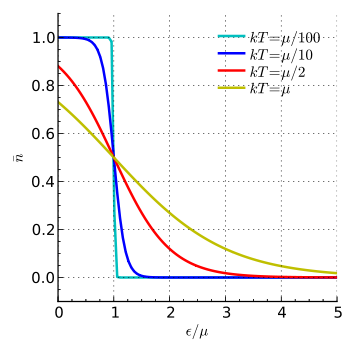
\includegraphics[width=300pt,keepaspectratio=true]{Addons/fermilowtemperature}
\caption{\footnotesize{Distribuzione di Fermi a temperature diverse.}}

\end{figure}

Passiamo adesso alla termodinamica. Nello sviluppo al secondo ordine di $\beta p$:
$$
\beta p=\frac{f_{5/2}(z)}{\lambda^3}=\frac{1}{\lambda^3}\frac{8}{15\sqrt{\pi}}\nu^{5/2}\left[1+\frac{5}{8}\pi^2\nu^{-2}\right]\;,
$$
sostituiamo lo sviluppo al secondo ordine di $\nu$ dato dalla \eqref{ch4_nu} per ottenere:
$$
\frac{pV}{kT}=\frac{V}{\left(\dfrac{2\pi\hbar^2}{mkT}\right)^{3/2}}\frac{8}{15\sqrt{\pi}}\left(\frac{\epsilon_F}{kT}\right)^{5/2}\left[1-\frac{5\pi^2}{24}\left(\frac{kT}{\epsilon_F}\right)^2+\frac{5\pi^2}{8}\left(\frac{kT}{\epsilon_F}\right)^2\right]\;,
$$
da cui ricaviamo l'equazione di stato per $kT\ll \epsilon_F$:
\begin{equation}
p=\frac{2}{5}\frac{N}{V}\epsilon_F\left[1+\frac{5\pi^2}{12}\left(\frac{kT}{\epsilon_F}\right)^2\right]\;.
\end{equation}
Per l'energia interna invece si ottiene:
\begin{equation}
E=\frac{3}{5}N\epsilon_F\left[1+\frac{5\pi^2}{12}\left(\frac{kT}{\epsilon_F}\right)^2\right]\;.
\end{equation}
Dall'energia interna possiamo calcolare il calore specifico:
\begin{equation}
\frac{C_v}{Nk}=\pdev{(E/Nk)}{T}=\frac{\pi^2}{2}\frac{kT}{\epsilon_F}\;,
\end{equation}
che è quindi lineare in $T$. \\
Consideriamo adesso il contributo di eventuali gradi di libertà interni (ad esempio, lo spin): ogni livello acquisirà una certa degenerazione $g$ ($=2s+1$ per particelle di spin $s$) e dunque:
$$
N=g\sum_{|\mathbf{p}|<p_F}\bra n_{\mathbf{p}}\ket=g\frac{V}{(2\pi\hbar)^3}4\pi\int_0^{p_F}\diff{p}\;p^2=\frac{gV}{6\pi^2\hbar^3}p_F^3\;,
$$
e quindi l'energia di Fermi diventa:
\begin{equation}
\epsilon_F=\frac{\hbar^2}{2m}\left(\frac{6\pi^2}{gv}\right)^{2/3}\;.
\end{equation}
Le altre formule sono identiche, a meno della sostituzione $v\to gv$.
\section{Gas di Fermi ideale in dimensione arbitraria}
Le equazioni di partenza sono le stesse del caso tridimensionale. Passando al limite termodinamico però, otteniamo in dimensione $d$ arbitraria:
\begin{align}
&\beta P=\frac{1}{(2\pi\hbar)^d}\int\diff^d{p}\;\ln\left(1+ze^{-\beta p^2/2m}\right)\;, \\
&\frac{\lambda}{v}=\frac{1}{(2\pi\hbar)^d}\int\diff^d{p}\frac{1}{z^{-1}e^{\beta p^2/2m}+1}\;.
\end{align}
Analogamente al caso bosonico,
$$
\int\diff^d{p}=s_d\int_0^{+\infty}\diff{p}\; p^{d-1}, \qquad s_d=\frac{2\pi^{d/2}}{\Gamma(d/2)}\;,
$$
da cui:
\begin{align}
&\beta P=\frac{1}{\lambda^d}f_{d/2+1}(z) \notag\;, \\
&\frac{1}{v}=\frac{1}{\lambda^d}f_{d/2}(z)\;,
\end{align}
con:
\begin{equation}
f_{d/2}(z)=\frac{s_d}{\pi^{d/2}}\int_0^{+\infty}\diff{x}\frac{x^{d-1}}{z^{-1}e^{x^2}+1}=\sum_{\ell=1}^{\infty}(-1)^{\ell+1}\frac{z^{\ell}}{\ell^{d/2}}\;.
\end{equation}
Eseguendo gli stessi passaggi del caso 3D, troviamo lo sviluppo di Sommerfeld di $f_{d/2}(z)$:
\begin{equation}
f_{d/2}(z)=\frac{s_d}{d\pi^{d/2}}(\ln z)^{d/2}\left[1+\frac{d(d-2)}{8}\frac{\pi^2}{3}(\ln z)^{-2}+\cdots\right]\;.
\end{equation}
Al primo ordine ($T=0$), posto $z=e^{\beta\epsilon_F}$, troviamo:
\begin{equation}
\epsilon_F=\frac{(2\pi\hbar)^2}{2m}\left(\frac{d}{s_d v}\right)^{2/d}\;.
\end{equation}
All'ordine successivo ($0<kT\ll \beta\epsilon_F$):
\begin{equation}
\frac{\epsilon_F}{kT}=\ln z\left[1+\frac{d(d-2)}{8}\frac{\pi^2}{3}(\ln z)^{-2}\right]^{2/d}\simeq \ln z\left[1+\frac{d-2}{4}\frac{\pi^2}{3}(\ln z)^{-2}\right]\;.
\end{equation}
Invertendo ordine per ordine si ha:
\begin{equation}
\ln z=\frac{\epsilon_F}{kT}\left[1-\frac{d-2}{4}\frac{\pi^2}{3}\left(\frac{kT}{\epsilon_F}\right)^2\right]\;.
\end{equation}
Allora:
\begin{align*}
\beta P &= \frac{f_{d/2+1}(z)}{\lambda^d}=\frac{1}{\lambda^d}\frac{s_{d+2}}{\pi^{d/2+1}(d+2)}(\ln z)^{d/2+1}\left[1+\frac{d(d+2)}{8}\frac{\pi^2}{3}(\ln z)^{-2}\right] \\
&=\frac{s_d}{d\pi^{d/2}}\frac{(\ln z)^{d/2+1}}{1+d/2}\left[1+\frac{d(d+2)}{8}\frac{\pi^2}{3}(\ln z)^{-2}\right]\;.
\end{align*}
L'equazione di stato segue pertanto dalla relazione:
\begin{align}
\beta Pv =\frac{f_{d/2+1}(z)}{f_{d/2}(z)} &= \frac{(\ln z)^{d/2+1}}{(\ln z)^{d/2}}\frac{1}{1+d/2}\left[1+\frac{d}{2}\frac{\pi^2}{3}(\ln z)^{-2}+\cdots \right] \notag \\
&= \ln z \frac{1}{1+d/2}\left[1+\frac{d}{2}\frac{\pi^2}{3}(\ln z)^{-2}+\cdots\right] \notag \\
&= \frac{\epsilon_F}{kT}\frac{1}{1+d/2}\left[1-\frac{\pi^2}{3}\left(\frac{kT}{\epsilon_F}\right)^2\frac{d+2}{4}+\cdots\right]\;.
\end{align}
Da quest'espressione possiamo calcolare l'energia interna $E=dPV/2$:
\begin{equation}
E=\frac{d/2}{1+d/2}N\epsilon_F\left[1+\frac{\pi^2}{3}\frac{d+2}{4}\left(\frac{kT}{\epsilon_F}\right)^2+\cdots\right]\;.
\end{equation}
Mentre per il calore specifico otteniamo:
\begin{equation}
\frac{c_v}{Nk}=\frac{\partial(E/Nk)}{\partial T}=\frac{d\pi^2}{6}\frac{kT}{\epsilon_F}\;.
\end{equation}

\section{Magnetismo}
Consideriamo un sistema statistico in presenza di un campo magnetico esterno $\mathbf{h}$. Il sistema acquista una magnetizzazione $\mathbf{M}$ lungo la direzione di $\mathbf{h}$. Definiamo la \emph{suscettività magnetica} come:
\begin{equation}
\chi\equiv \left.\pdev{M}{h}\right|_{h=0}\;.
\end{equation}
A seconda del segno della suscettività distinguiamo due fenomeni: \emph{diamagnetismo} per $\chi<0$ e  \emph{paramagnetismo} per $\chi>0$. Per $h=|\mathbf{h}|$ sufficientemente piccolo, vale la risposta lineare:
\begin{equation}
H=H_0-VhM\;,
\end{equation}
da cui:
\begin{align}
&\boxed{M=\frac{1}{V}\left\langle -\pdev{H}{h}\right\rangle} &\mbox{Teorema di Hellmann-Feynman}\;.
\end{align}
In particolare,
\begin{align*}
& M=kT\left(\frac{\partial}{\partial h}\frac{\ln \zpart_N}{V}\right)_{T,V} & \mbox{ensemble canonico}\;, \\
& M=kT\left(\frac{\partial}{\partial h}\frac{\ln\zpart}{V}\right)_{T,V,N} & \mbox{ensemble grancanonico}\;.
\end{align*}
L'effetto del campo magnetico sul nucleo è trascurabile, in quanto il momento magnetico intrinseco del nucleo è $10^3$ volte più piccolo rispetto a quello degli elettroni. Tutto il magnetistmo pertanto dipende dagli elettroni. Gli effetti di un campo magnetico esterno sugli elettroni sono due:
\begin{enumerate}
\item gli elettroni si muovono su orbite quantizzate (livelli di Landau) $\Longrightarrow$ DIAMAGNETISMO;
\item gli spin tendono ad allinearsi con il campo magnetico $\Longrightarrow$ PARAMAGNETISMO.
\end{enumerate}

\section{Diamagnetismo di Landau}
\begin{thm} In Meccanica Classica il diamagnetismo non esiste.
\end{thm}
\proof La forza sugli elettroni esercitata da un campo magnetico $\mathbf{h}$ è data dalla forza di Lorentz, $\mathbf{F}_L=e\mathbf{v}\wedge\mathbf{h}$. Il lavoro compiuto dalla forza è di conseguenza:
$$
L=\mathbf{F}_L\cdot\mathbf{v}=e(\mathbf{v}\wedge\mathbf{h})\cdot\mathbf{v}=0\;.
$$
Se il lavoro è nullo, la variazione di energia dovuta a $\mathbf{h}$ è $\Delta E=0$ e pertanto:
$$
M=\left\langle\pdev{H}{h}\right\rangle=0\;.
$$
\endproof
Per avere diamagnetismo c'è bisogno della Meccanica Quantistica. Consideriamo un elettrone in campo magnetico esterno. Trascurando lo spin, l'Hamiltoniana del sistema è:
\begin{equation}
H=\frac{1}{2m}\left(\mathbf{p}+\frac{e}{c}\mathbf{A}\right)^2\;.
\end{equation}
Sia $\mathbf{h}=(0,0,h)$ e scegliamo per il potenziale vettore la gauge $\mathbf{A}=(-yh,0,0)$. Allora:
\begin{equation}
H=\frac{1}{2m}\left[\left(p_x-\frac{eh}{c}y\right)^2+p_y^2+p_z^2\right]\;.
\end{equation}
Notando che $H$ non dipende dalle coordinate $x,z$, possiamo cercare una soluzione dell'equazione di \Sch\; della forma:
\begin{equation}
\psi(x,y,z)=e^{-ik_xx-ik_zz}\varphi(y)\;,
\end{equation}
con $p_x=\hbar k_x,p_z=\hbar k_z$. L'equazione per $\varphi$ è dunque:
\begin{align*}
&\left[\frac{1}{2m}\left(\hbar k_x-\frac{eh}{c}y\right)^2+\frac{p_y^2}{2m}+\frac{\hbar^2k_z^2}{2m}\right]\varphi(y)=E\varphi(y)\;, \\
&\left[\frac{p_y^2}{2m}+\frac{1}{2}m\left(\frac{eh}{mc}y-\frac{\hbar k_x}{m}\right)^2\right]\varphi(y)=\left(E-\frac{\hbar^2k_z^2}{2m}\right)\varphi(y)\;.
\end{align*}
Siano adesso:
\begin{align}
&\omega_0\equiv \frac{eh}{mc}\;, \\
&y_0\equiv \frac{\hbar k_x}{m\omega_0}=\frac{\hbar c}{eh}k_x\;.
\end{align}
L'equazione diventa quindi:
\begin{equation}
\left[\frac{p_y^2}{2m}+\frac{1}{2}m\omega_0^2(y-y_0)^2\right]\varphi(y)=\left(E-\frac{\hbar^2 k_z^2}{2m}\right)\varphi(y)\;.
\end{equation}
Riconosciamo quindi che $\varphi$ obbedisce all'equazione di \Sch\; di un oscillatore armonico, i cui livelli energetici sono noti e dati da
\begin{equation}
\epsilon_j=\hbar\omega_0\left(j+\frac{1}{2}\right),\qquad j=0,1,\ldots\;.
\end{equation}
Essendo quindi $E-\hbar^2k_z^2/2m=\epsilon_j$, troviamo infine l'espressione per i livelli energetici di Landau:
\begin{equation}
\boxed{E_j=\frac{\hbar^2k_z^2}{2m}+\hbar\omega_0\left(j+\frac{1}{2}\right)}\;.
\end{equation}
Se la particella si trova in una scatola di lato $L=V^{1/3}$ con condizioni periodiche al contorno, allora $k_x$ è quantizzato:
\begin{equation}
k_x=\frac{2\pi}{L}n_x\;,
\end{equation}
ma non tutti gli $n_x$ sono possibili. La coordinata $y_0$ che abbiamo definito è vincolata a stare nel sistema, i.e. $y_0\in [0,L]$. Possiamo quindi scrivere:
$$
0\le y_0=\frac{\hbar c}{eh}k_x=\frac{\hbar c}{eh}\frac{2\pi}{L}n_x\le L\;,
$$
da cui segue $n_x>0$ e inoltre:
\begin{equation}
n_x\le \frac{eh}{\hbar c}\frac{L^2}{2\pi}\equiv g\;,
\end{equation}
dove $g$ è la degenerazione dei livelli di Landau. Notiamo che $g\propto L^2$, infatti abbiamo una superficie di orbite degeneri (una direzione è fissata dal campo magnetico). \\
Dimostriamo adesso che i livelli di Landau sono l'origine fisica del diamagnetismo. Scriviamo la funzione di partizione di un  gas di elettroni senza spin nell'ensemble grancanonico:
$$
\zpart=\prod_{\lambda}\left(1+ze^{-\beta\epsilon_{\lambda}}\right),\qquad \lambda=\{p_z,j,\alpha\}\;,
$$
dove $\alpha=1,\ldots,g$ conta la degenerazione. Prendendo il logaritmo otteniamo:
\begin{align*}
\ln\zpart &= \sum_{\alpha=1}^g\sum_{j=0}^{\infty}\sum_{p_z}\ln\left(1+ze^{-\beta\epsilon(p_z,j)}\right) \\
&=  g\frac{L}{2\pi\hbar}\int_0^{+\infty}\diff{p_z}\;\sum_{j=0}^{\infty}\ln\left(1+ze^{-\beta\epsilon(p_z,j)}\right)\;.
\end{align*}
Mentre il numero medio di particelle è:
$$
N=z\frac{\partial}{\partial z}\ln\zpart=\frac{gL}{2\pi\hbar}\sum_{j=0}^{\infty}\int_0^{+\infty}\diff{p_z}\;\frac{1}{z^{-1}e^{\beta\epsilon(p_z,j)}+1}\;.
$$
Da questa espressione dovremmo in linea teorica ricavare $z$ in funzione di $N$, la qual cosa è piuttosto complicata. Possiamo tuttavia studiare il limite di alte temperature $T\to\infty \;\Longleftrightarrow\; z\to 0$. Allora, al primo ordine:
\begin{align*}
\ln\zpart&=\frac{gL}{2\pi\hbar}z\sum_{j=0}^{\infty}\int_0^{+\infty}\diff{p}\;e^{-\beta(p^2/2m+\hbar\omega_0(j+1/2))} \\
&= \frac{gL}{2\pi\hbar}z\sum_{j=0}^{\infty}e^{-\beta\hbar\omega_0(j+1/2)}\int_0^{+\infty}\diff{p}\;e^{-\beta p^2/2m} \\
&= \frac{gL}{2\pi\hbar}z\sqrt{\frac{2\pi m}{\beta}}\frac{1}{2}\frac{e^{-\beta\hbar\omega_0/2}}{1-e^{-\beta\hbar\omega_0}} \\
&\equiv \frac{gLz}{\lambda}\frac{e^{-x}}{1-e^{-2x}},\qquad x=\frac{\beta\hbar\omega_0}{2}\;.
\end{align*}
Nel limite di alta temperatura sarà anche $x\ll 1$, quindi sviluppiamo:
\begin{equation}
\frac{e^{-x}}{1-e^{-2x}}=\frac{1}{e^x-e^{-x}}=\frac{1}{\sinh x}\simeq \frac{1}{2\left(x+\dfrac{x^3}{6}\right)}\simeq \frac{1}{2x}\left(1-\frac{x^2}{6}\right)\;.
\end{equation}
Allora:
\begin{align}
\ln\zpart &\simeq \frac{zgL}{\lambda}\frac{1}{2x}\left(1-\frac{x^2}{6}\right) \notag \\
&= \frac{zL}{\lambda}\cdot \frac{eh}{\hbar c}\cdot\frac{L^2}{2\pi}\frac{1}{\beta\hbar\dfrac{eh}{mc}}\left(1-\frac{1}{24}(\beta\hbar\omega_0)^2\right) \notag \\
&=\frac{zV}{\lambda^3}\left[1-\frac{1}{24}\left(\frac{\hbar\omega_0}{kT}\right)^2\right]\qquad\qquad V=L^3\;,
\end{align}
che al primo ordine coincide con il risultato classico. Per quanto riguarda la magnetizzazione, si ha:
\begin{align}
M &= kT\frac{\partial}{\partial h}\frac{\ln\zpart}{V}=-\frac{z}{\lambda^3}\frac{kT}{24}\frac{\hbar^2}{(kT)^2}2\omega_0\pdev{\omega_0}{h} \notag \\
&= -\frac{z}{\lambda^3}\frac{1}{24}\frac{\hbar^2}{kT}2\frac{eh}{mc}\frac{e}{mc} \notag \\
&= -h\frac{z}{3kT\lambda^3}\left(\frac{e\hbar}{2mc}\right)^2\equiv \chi h\;,
\end{align}
dove $\chi$ è la suscettività magnetica. Per eliminare $z$, usiamo la formula classica: $z=\lambda^3\dfrac{N}{V}$. Quindi:
\begin{equation}
\chi=-\frac{N}{3kTV}\left(\frac{e\hbar}{2mc}\right)^2\;.
\end{equation}
Notiamo che $\chi<0$, in accordo con il fatto che stiamo trattando il diamagnetismo e che $\chi\propto T^{-1}$, in accordo con la legge di Curie. \\
\subsection{Effetto De Haas - Van Alphen}
Il limite di basse temperature è difficile da trattare. Consideriamo solamente il caso $T=0$, in cui avviene il cosidetto \emph{effetto De Haas-Van Alphen}. Faremo due assunzioni:
\begin{enumerate}
\item $T=0$, cioè $kT\ll \hbar\omega_0$;
\item la terza dimensione $\hat{\mathbf{z}}$ non esiste.
\end{enumerate}
I livelli energetici sono quelli di Landau con $\mathbf{p}^2=0$ (temperatura nulla): $\epsilon_j=\hbar\omega_0(j+1/2)\equiv 2\mu_0 h(j+1/2)$, dove:
\begin{equation}
\mu_0=\frac{e\hbar}{2mc}\;,
\end{equation}
è il magnetone di Bohr. La degenerazione dei livelli sarà:
$$
g=N\frac{h}{h_0},\qquad h_0=\frac{2\pi n\hbar c}{e},\qquad  n=\frac{N}{L^2}\;,
$$
dove $n$ è la densità dimensionale e $h_0$ è il valore del campo magnetico per cui, se $h>h_0$, tutte le particelle sono nello stato fondamentale (infatti $g>N$). Allora, per calcolare l'energia dello stato fondamentale dobbiamo distinguere due casi: se $h>h_0$, per quanto detto, $E_0=N\epsilon_0=N\mu_0h$. Se $h<h_0$, alcune particelle devono andare negli stati eccitati. Supponiamo, senza perdere generalità, che $h$ sia tale che i primi $j$ livelli siano completamente occupati, il $j+1$-esimo lo sia parzialmente e quelli da $j+2$ in poi non siano occupati. In questo caso $g(j+1)<N<g(j+2)$, che si può scrivere come:
\begin{equation}
\frac{1}{j+2}<\frac{g}{N}\equiv\frac{h}{h_0}<\frac{1}{j+1}\;.
\end{equation}
In questo caso l'energia dello stato fondamentale sarà:
\begin{align}
E_0 &= g\sum_{i=0}^j\epsilon_i+[N-(j+1)g]\epsilon_{j+1} \notag \\
&= 2\mu_0 h\left[g\sum_{i=0}^j\left(i+\frac{1}{2}\right)+(N-(j+1)g)\left(j+\frac{3}{2}\right)\right] \notag \\
&= 2\mu_0 h\left[\frac{1}{2}(j+1)^2\frac{Nh}{h_0}+\left(N-(j+1)\frac{Nh}{h_0}\right)\left(j+\frac{3}{2}\right)\right] \notag \\
&=\mu_0hN\left[(2j+3)+\frac{h}{h_0}\left((j+1)^2-(j+1)(2j+3)\right)\right] \notag \\
&=\mu_0hN\left[(2j+3)+\frac{h}{h_0}(j+1)(j+2)\right]\;.
\end{align}
Per la magnetizzazione otteniamo di conseguenza:
\begin{equation}
M=\frac{1}{V}\left(-\pdev{E_0}{h}\right)=-\frac{n}{N}\pdev{E_0}{h}=\begin{cases}
-\mu_0 n\qquad\qquad h>h_0\;, \\
\\
\mu_0 n\left[2(j+1)(j+2)\dfrac{h}{h_0}-(2j+3)\right]\qquad \dfrac{1}{j+2}<\dfrac{h}{h_0}<\dfrac{1}{j+1}\;.
\end{cases}
\end{equation}

\begin{center}
\begingroup
  \makeatletter
  \providecommand\color[2][]{%
    \GenericError{(gnuplot) \space\space\space\@spaces}{%
      Package color not loaded in conjunction with
      terminal option `colourtext'%
    }{See the gnuplot documentation for explanation.%
    }{Either use 'blacktext' in gnuplot or load the package
      color.sty in LaTeX.}%
    \renewcommand\color[2][]{}%
  }%
  \providecommand\includegraphics[2][]{%
    \GenericError{(gnuplot) \space\space\space\@spaces}{%
      Package graphicx or graphics not loaded%
    }{See the gnuplot documentation for explanation.%
    }{The gnuplot epslatex terminal needs graphicx.sty or graphics.sty.}%
    \renewcommand\includegraphics[2][]{}%
  }%
  \providecommand\rotatebox[2]{#2}%
  \@ifundefined{ifGPcolor}{%
    \newif\ifGPcolor
    \GPcolorfalse
  }{}%
  \@ifundefined{ifGPblacktext}{%
    \newif\ifGPblacktext
    \GPblacktexttrue
  }{}%
  % define a \g@addto@macro without @ in the name:
  \let\gplgaddtomacro\g@addto@macro
  % define empty templates for all commands taking text:
  \gdef\gplbacktext{}%
  \gdef\gplfronttext{}%
  \makeatother
  \ifGPblacktext
    % no textcolor at all
    \def\colorrgb#1{}%
    \def\colorgray#1{}%
  \else
    % gray or color?
    \ifGPcolor
      \def\colorrgb#1{\color[rgb]{#1}}%
      \def\colorgray#1{\color[gray]{#1}}%
      \expandafter\def\csname LTw\endcsname{\color{white}}%
      \expandafter\def\csname LTb\endcsname{\color{black}}%
      \expandafter\def\csname LTa\endcsname{\color{black}}%
      \expandafter\def\csname LT0\endcsname{\color[rgb]{1,0,0}}%
      \expandafter\def\csname LT1\endcsname{\color[rgb]{0,1,0}}%
      \expandafter\def\csname LT2\endcsname{\color[rgb]{0,0,1}}%
      \expandafter\def\csname LT3\endcsname{\color[rgb]{1,0,1}}%
      \expandafter\def\csname LT4\endcsname{\color[rgb]{0,1,1}}%
      \expandafter\def\csname LT5\endcsname{\color[rgb]{1,1,0}}%
      \expandafter\def\csname LT6\endcsname{\color[rgb]{0,0,0}}%
      \expandafter\def\csname LT7\endcsname{\color[rgb]{1,0.3,0}}%
      \expandafter\def\csname LT8\endcsname{\color[rgb]{0.5,0.5,0.5}}%
    \else
      % gray
      \def\colorrgb#1{\color{black}}%
      \def\colorgray#1{\color[gray]{#1}}%
      \expandafter\def\csname LTw\endcsname{\color{white}}%
      \expandafter\def\csname LTb\endcsname{\color{black}}%
      \expandafter\def\csname LTa\endcsname{\color{black}}%
      \expandafter\def\csname LT0\endcsname{\color{black}}%
      \expandafter\def\csname LT1\endcsname{\color{black}}%
      \expandafter\def\csname LT2\endcsname{\color{black}}%
      \expandafter\def\csname LT3\endcsname{\color{black}}%
      \expandafter\def\csname LT4\endcsname{\color{black}}%
      \expandafter\def\csname LT5\endcsname{\color{black}}%
      \expandafter\def\csname LT6\endcsname{\color{black}}%
      \expandafter\def\csname LT7\endcsname{\color{black}}%
      \expandafter\def\csname LT8\endcsname{\color{black}}%
    \fi
  \fi
    \setlength{\unitlength}{0.0500bp}%
    \ifx\gptboxheight\undefined%
      \newlength{\gptboxheight}%
      \newlength{\gptboxwidth}%
      \newsavebox{\gptboxtext}%
    \fi%
    \setlength{\fboxrule}{0.5pt}%
    \setlength{\fboxsep}{1pt}%
\begin{picture}(7200.00,5040.00)%
    \gplgaddtomacro\gplbacktext{%
      \csname LTb\endcsname%
      \put(682,704){\makebox(0,0)[r]{\strut{}}}%
      \put(682,4379){\makebox(0,0)[r]{\strut{}}}%
      \put(682,1623){\makebox(0,0)[r]{\strut{}$-1$}}%
      \put(682,2542){\makebox(0,0)[r]{\strut{}$0$}}%
      \put(682,3460){\makebox(0,0)[r]{\strut{}$1$}}%
      \put(1563,484){\makebox(0,0){\strut{}$\frac{1}{4}$}}%
      \put(1802,484){\makebox(0,0){\strut{}$\frac{1}{3}$}}%
      \put(2311,484){\makebox(0,0){\strut{}$\frac{1}{2}$}}%
      \put(6803,484){\makebox(0,0){\strut{}}}%
      \put(814,484){\makebox(0,0){\strut{}$0$}}%
      \put(3809,484){\makebox(0,0){\strut{}$1$}}%
      \csname LTb\endcsname%
      \put(3809,3552){\makebox(0,0)[l]{\strut{} \small $j=0$}}%
      \put(2311,3552){\makebox(0,0)[l]{\strut{} \small $j=1$}}%
      \put(1802,3552){\makebox(0,0)[l]{\strut{} \small $j=2$}}%
    }%
    \gplgaddtomacro\gplfronttext{%
      \csname LTb\endcsname%
      \put(176,2541){\rotatebox{-270}{\makebox(0,0){\strut{}$M/(\mu_0 n)$}}}%
      \put(3808,154){\makebox(0,0){\strut{}$h/h_0$}}%
      \put(3808,4709){\makebox(0,0){\strut{}Magnetizzazione nell'effetto de Haas-Van Alphen}}%
    }%
    \gplbacktext
    \put(0,0){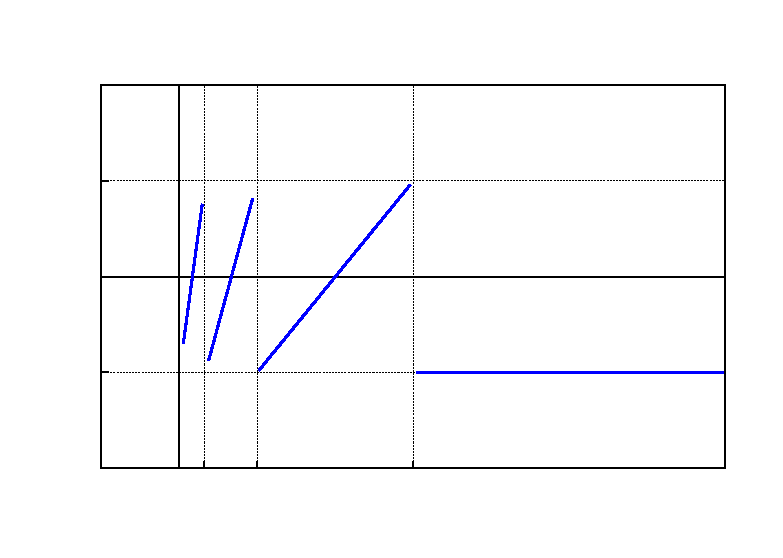
\includegraphics{Addons/magnetizzazione}}%
    \gplfronttext
  \end{picture}%
\endgroup
\end{center}

Per quanto riguarda la suscettività, abbiamo:
\begin{equation}
\chi=\begin{cases}
0,\qquad h>h_0\;, \\
\\
\dfrac{2\mu_0 n}{h_0}(j+1)(j+2),\qquad \dfrac{1}{j+2}<\dfrac{h}{h_0}<\dfrac{1}{j+1}\;.
\end{cases}
\end{equation}

\begin{center}
\begingroup
  \makeatletter
  \providecommand\color[2][]{%
    \GenericError{(gnuplot) \space\space\space\@spaces}{%
      Package color not loaded in conjunction with
      terminal option `colourtext'%
    }{See the gnuplot documentation for explanation.%
    }{Either use 'blacktext' in gnuplot or load the package
      color.sty in LaTeX.}%
    \renewcommand\color[2][]{}%
  }%
  \providecommand\includegraphics[2][]{%
    \GenericError{(gnuplot) \space\space\space\@spaces}{%
      Package graphicx or graphics not loaded%
    }{See the gnuplot documentation for explanation.%
    }{The gnuplot epslatex terminal needs graphicx.sty or graphics.sty.}%
    \renewcommand\includegraphics[2][]{}%
  }%
  \providecommand\rotatebox[2]{#2}%
  \@ifundefined{ifGPcolor}{%
    \newif\ifGPcolor
    \GPcolorfalse
  }{}%
  \@ifundefined{ifGPblacktext}{%
    \newif\ifGPblacktext
    \GPblacktexttrue
  }{}%
  % define a \g@addto@macro without @ in the name:
  \let\gplgaddtomacro\g@addto@macro
  % define empty templates for all commands taking text:
  \gdef\gplbacktext{}%
  \gdef\gplfronttext{}%
  \makeatother
  \ifGPblacktext
    % no textcolor at all
    \def\colorrgb#1{}%
    \def\colorgray#1{}%
  \else
    % gray or color?
    \ifGPcolor
      \def\colorrgb#1{\color[rgb]{#1}}%
      \def\colorgray#1{\color[gray]{#1}}%
      \expandafter\def\csname LTw\endcsname{\color{white}}%
      \expandafter\def\csname LTb\endcsname{\color{black}}%
      \expandafter\def\csname LTa\endcsname{\color{black}}%
      \expandafter\def\csname LT0\endcsname{\color[rgb]{1,0,0}}%
      \expandafter\def\csname LT1\endcsname{\color[rgb]{0,1,0}}%
      \expandafter\def\csname LT2\endcsname{\color[rgb]{0,0,1}}%
      \expandafter\def\csname LT3\endcsname{\color[rgb]{1,0,1}}%
      \expandafter\def\csname LT4\endcsname{\color[rgb]{0,1,1}}%
      \expandafter\def\csname LT5\endcsname{\color[rgb]{1,1,0}}%
      \expandafter\def\csname LT6\endcsname{\color[rgb]{0,0,0}}%
      \expandafter\def\csname LT7\endcsname{\color[rgb]{1,0.3,0}}%
      \expandafter\def\csname LT8\endcsname{\color[rgb]{0.5,0.5,0.5}}%
    \else
      % gray
      \def\colorrgb#1{\color{black}}%
      \def\colorgray#1{\color[gray]{#1}}%
      \expandafter\def\csname LTw\endcsname{\color{white}}%
      \expandafter\def\csname LTb\endcsname{\color{black}}%
      \expandafter\def\csname LTa\endcsname{\color{black}}%
      \expandafter\def\csname LT0\endcsname{\color{black}}%
      \expandafter\def\csname LT1\endcsname{\color{black}}%
      \expandafter\def\csname LT2\endcsname{\color{black}}%
      \expandafter\def\csname LT3\endcsname{\color{black}}%
      \expandafter\def\csname LT4\endcsname{\color{black}}%
      \expandafter\def\csname LT5\endcsname{\color{black}}%
      \expandafter\def\csname LT6\endcsname{\color{black}}%
      \expandafter\def\csname LT7\endcsname{\color{black}}%
      \expandafter\def\csname LT8\endcsname{\color{black}}%
    \fi
  \fi
    \setlength{\unitlength}{0.0500bp}%
    \ifx\gptboxheight\undefined%
      \newlength{\gptboxheight}%
      \newlength{\gptboxwidth}%
      \newsavebox{\gptboxtext}%
    \fi%
    \setlength{\fboxrule}{0.5pt}%
    \setlength{\fboxsep}{1pt}%
\begin{picture}(7200.00,5040.00)%
    \gplgaddtomacro\gplbacktext{%
      \csname LTb\endcsname%
      \put(682,1269){\makebox(0,0)[r]{\strut{}2}}%
      \put(682,2400){\makebox(0,0)[r]{\strut{}6}}%
      \put(682,4096){\makebox(0,0)[r]{\strut{}12}}%
      \put(682,704){\makebox(0,0)[r]{\strut{}$0$}}%
      \put(1563,484){\makebox(0,0){\strut{}$\frac{1}{4}$}}%
      \put(1802,484){\makebox(0,0){\strut{}$\frac{1}{3}$}}%
      \put(2311,484){\makebox(0,0){\strut{}$\frac{1}{2}$}}%
      \put(6803,484){\makebox(0,0){\strut{}}}%
      \put(814,484){\makebox(0,0){\strut{}$0$}}%
      \put(3809,484){\makebox(0,0){\strut{}$1$}}%
    }%
    \gplgaddtomacro\gplfronttext{%
      \csname LTb\endcsname%
      \put(176,2541){\rotatebox{-270}{\makebox(0,0){\strut{}$h_0\chi/(2\mu_0 n)$}}}%
      \put(3808,154){\makebox(0,0){\strut{}$h/h_0$}}%
      \put(3808,4709){\makebox(0,0){\strut{}Suscettività nell'effetto de Haas-Van Alphen}}%
    }%
     \gplbacktext
    \put(0,0){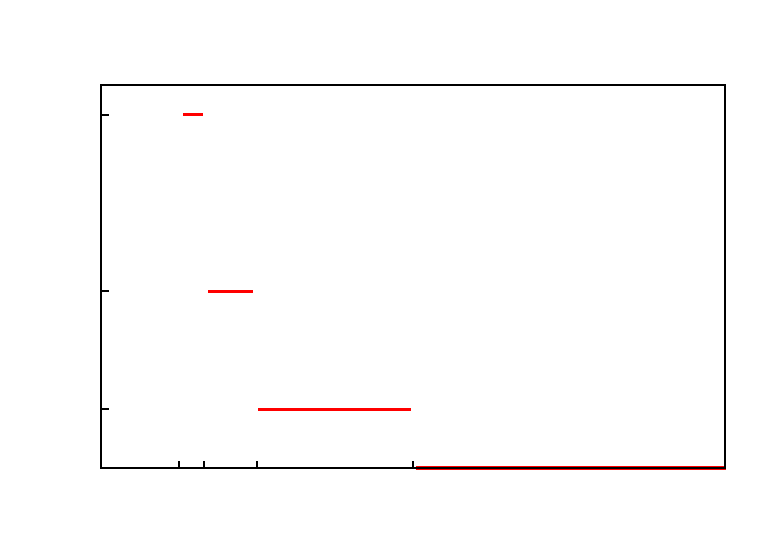
\includegraphics{Addons/suscettivita}}%
    \gplfronttext
  \end{picture}%
\endgroup
\end{center}

\section{Paramagnetismo}
Il paramagnetismo consiste nell'allineamento degli spin in presenza di campo magnetico, quindi lo spin non può essere trascurato. L'Hamiltoniana di una carica avente spin $1/2$ in presenza di campo esterno $\mathbf{h}$ è:
\begin{equation}
H=\frac{1}{2m}\left(\mathbf{p}-\frac{e}{c}\mathbf{A}\right)-\mu_B\boldsymbol{\sigma}\cdot\mathbf{h}\;.
\end{equation}
Seguendo lo schema di Pauli, trascuriamo $\mathbf{A}$ e scegliamo l'asse $\hat{\mathbf{z}}$ lungo $\mathbf{h}$: i livelli energetici saranno dunque:
\begin{equation}
\epsilon_{\mathbf{p},s}=\frac{\mathbf{p}^2}{2m}-s\mu_bh,\qquad\qquad s=\pm 1\;.
\end{equation}
Essendo fermioni, i numeri di occupazione possibili saranno $n_{\mathbf{p},s}=0,1$. Allora l'energia media e il numero medio di particelle si scriveranno come:
\begin{align}
E&=\sum_{\mathbf{p},s}\epsilon_{\mathbf{p},s}n_{\mathbf{p},s}=\sum_{\mathbf{p}}\left[\left(\frac{\mathbf{p}^2}{2m}-\mu_Bh\right)n_{\mathbf{p}}^++\left(\frac{\mathbf{p}^2}{2m}+\mu_Bh\right)n_{\mathbf{p}}^-\right] \\
N&=\sum_{\mathbf{p},s}n_{\mathbf{p},s}=\sum_{\mathbf{p}}\left(n_{\mathbf{p}}^++n_{\mathbf{p}}^-\right)\equiv N_++N_-\;.
\end{align}
La funzione di partizione è quindi:
\begin{equation}
Z_N=\sum_{\{n_{\mathbf{p}}^+\},\{n_{\mathbf{p}}^-\}}\exp\left[-\beta\left(\sum_{\mathbf{p}}\frac{\mathbf{p}^2}{2m}(n_{\mathbf{p}}^++n_{\mathbf{p}}^-)-\mu_Bh(N_+-N_-)\right)\right]\;,
\end{equation}
con il vincolo $\sum_{\mathbf{p}}(n_{\mathbf{p}}^++n_{\mathbf{p}}^-)=N$. A questo punto fissiamo $N_+$ e sommiamo su tutti gli $n_{\mathbf{p}}^+$ tali che $\sum_{\mathbf{p}}n_{\mathbf{p}}^+=N_+$ e solo dopo sommiamo su $N_+$. Allora:
\begin{align}
Z_N &= \sum_{N_+=0}^N e^{\beta\mu_B h(2N_+-N)}\sum_{\{n_{\mathbf{p}}^+\}}\exp\left[-\beta\sum_{\mathbf{p}}\frac{\mathbf{p}^2}{2m}n_{\mathbf{p}}^+\right]\sum_{\{n_{\mathbf{p}}^-\}}\exp\left[-\beta\sum_{\mathbf{p}}\frac{\mathbf{p}^2}{2m}n_{\mathbf{p}}^-\right] \notag \\
&= e^{-\beta\mu_BhN}\sum_{N_+=0}^Ne^{2\beta\mu_BhN_+}Z_{N_+}^0Z_{N-N_+}^0 \notag \\
&= e^{-\beta\mu_BhN}\sum_{N_+=0}^Ne^{[2\beta\mu_0hN_+-\beta F_0(N_+)-\beta F_0(N-N_+)]}\;,
\end{align}
dove $Z_N^0$ indica la funzione di partizione di $N$ particelle senza spin e $F_0(N)$ è l'energia libera associata ad essa. Notiamo che:
$$
\frac{1}{N}\ln Z_N=-\beta\mu_Bh+\frac{1}{N}\ln\left[\sum_{N_+=0}^Ne^{2\beta\mu_BhN_+-\beta F_0(N_+)-\beta F_0(N-N_+)}\right]\;.
$$
Sia $\overline{N}_+$ il valore di $N_+$ che massimizza la somma:
\begin{align*}
\frac{1}{N}\ln Z_N &=\beta f(N)\;, \\
f(N) &= \mu_Bh\left(2\frac{N_+}{N}-1\right)-\frac{1}{N}\left(F_0(N_+)+F_0(N-N_+)\right)\;.
\end{align*}
Allora il massimo di $Z_N$ corrisponde al minimo di $f(N_+)$:
$$
\left.\pdev{f}{N_+}\right|_{N_+=\overline{N}_+}=0=2\mu_Bh-\left.\pdev{F}{N'}\right|_{N'=\overline{N}_+}-\left.\pdev{F(N-N')}{N'}\right|_{N'=\overline{N}_+}\;,
$$
da cui:
\begin{equation}
2\mu_Bh=\mu_0(\overline{N}_+)+\mu_0(N-\overline{N}_+)\;, \label{ch4_2mubh}
\end{equation}
dove $\mu_0$ è il potenziale chimico di particelle senza spin. Dalla \eqref{ch4_2mubh} siamo in grado di determinare $\overline{N}_+$, che ci consente di calcolare la magnetizzazione come:
\begin{equation}
M=\frac{\mu_B}{V}(2\overline{N}_+-N)\;.
\end{equation}
Se $kT\ll\epsilon_F$, allora $\mu_0(N)\equiv \epsilon_F(N)=\left(\dfrac{6\pi^2N}{V}\right)^{2/3}\dfrac{\hbar^2}{2m}$ all'ordine zero, mentre all'ordine $T^2$:
\begin{equation}
\mu_0(N)=\epsilon_F(N)\left[1-\frac{\pi^2}{12}\left(\frac{kT}{\epsilon_F}\right)^2\right]\;.
\end{equation}
In questo limite, l'equazione \eqref{ch4_2mubh} diventa:
\begin{equation}
2\mu_Bh=\epsilon_F(N_+)-\epsilon_F(N-N_+)-\frac{\pi^2}{12}(kT)^2\left[\frac{1}{\epsilon_F^2(N_+)}-\frac{1}{\epsilon_F^2(N-N_+)}\right]\;. \label{ch4_2mubh2}
\end{equation}
Introduciamo la polarizzazione $r$, definita come:
\begin{equation}
r\equiv 2\frac{N_+}{N}-1\;.
\end{equation}
In termini di polarizzazione, la magnetizzazione si scrive $M=\mu_BNr/V$. Inoltre, la \eqref{ch4_2mubh2} diventa:
$$
\frac{2\mu_Bh}{\epsilon_F}=(1+r)^{2/3}-(1-r)^{2/3}-\frac{\pi^2}{12}\left(\frac{kT}{\epsilon_F}\right)^2\left[(1+r)^{-2/3}-(1-r)^{-2/3}\right]\;.
$$
A $T=0$ il secondo termine si annulla:
$$
(1+r)^{2/3}-(1-r)^{2/3}=\frac{2\mu_Bh}{\epsilon_F}\;.
$$
Per $kT\ll \epsilon_F$ sviluppo le potenze in serie, ottenendo al primo ordine:
\begin{equation}
r=\frac{3}{2}\frac{\mu_Bh}{\epsilon_F}\;,
\end{equation}
mentre, per la magnetizzazione e la suscettività:
\begin{align}
M&=\frac{3}{2}\frac{\mu_B^2N}{\epsilon_FV}h\;, \notag \\
\chi &= \frac{3}{2}\frac{\mu_B^2N}{\epsilon_FV}\;.
\end{align}
Notiamo che $\chi>0$, in accordo con il fatto che stiamo trattando il paramagnetismo. Infine, osserviamo che per $T\to\infty$, sostituendo $\mu(N)=kT\ln(\lambda^3N/V)$ nella \eqref{ch4_2mubh}, ritroviamo il risultato classico  $\chi=N\mu_B^2/(VkT)$.
\chapter{Transizioni di fase}
Le transizioni di fase definiscono un cambio macroscopico di un sistema al variare di un parametro esterno. A parte la transizione di fase di un condensato di Bose-Einstein, tutte le transizioni di fase necessitano di interazioni. \\
Rigorosamente, una transizione di fase è caratterizzata da una singolarità, nel limite termodinamico, in un potenziale termodinamico, ad esempio $F=U-TS$ oppure $G=H-TS$. \\

\textbf{Classificazione di Ehrenfest}: se tutte le derivate di $F$ (o di $G$) fino all'ordine $n-1$ sono continue e la derivata $n$-esima è discontinua, allora la transizione è di ordine $n$.
\section{Transizioni del primo ordine}
Le transizioni del primo ordine sono caratterizzate da una discontinuità nella derivata prima dei potenziali termodinamici al variare dei parametri esterni $T$ oppure $p$:
\begin{align*}
-\left(\pdev{F}{T}\right)_V &=S\;, \\
\left(\pdev{G}{p}\right)_T &=V\;.
\end{align*}
Quindi una discontinuità nell'entropia oppure nel volume segnala una transizione di fase del primo ordine. Se chiamiamo 1 e 2 le due fasi, dato che $G$ è continuo, deve essere:
$$
\diff{G}(1)=\diff{G}(2)\qquad \Longrightarrow\qquad -S_1\diff{T}+V_1\diff{p}=-S_2\diff{T}+V_2\diff{p}\;,
$$
da cui:
\begin{equation}
\dev{p}{T}=\frac{S_2-S_1}{V_2-V_1}\equiv \frac{L}{T\Delta V}\;.
\end{equation}
Ritroviamo quindi l'equazioni di Clapeyron ($L$ è il calore latente).
\section{Transizioni del secondo ordine}
Le transizioni di fase del secondo ordine sono caratterizzate da derivate prime continue dei potenziali (quindi entropia e volume continui), mentre le derivate seconde sono discontinue. Ad esempio:
\begin{align*}
C_v&=-T\left(\pdev[2]{F}{T}\right)_V\;, \\
\kappa_T&=-\frac{1}{V}\left(\pdev[2]{G}{p}\right)_T\;.
\end{align*}
Le transizioni di fase del secondo ordine sono connesse con il fenomeno della \underline{rottura spontenea di simmetria} e con la \underline{crescita continua di un parametro d'ordine}.
\section{Modello di Ising}
Consideriamo un reticolo $d$ dimensionale in cui vi siano $N$ siti. Ogni sito è caratterizzato da una variabile di spin $s_i$ che può assumere i valori $\pm 1$. L'Hamiltoniana del modello è:
\begin{equation}
H=-J\sum_{\bra i,j\ket}s_is_j-h\sum_is_i\;,
\end{equation}
dove $J$ è l'accoppiamento tra le variabili. Se $J>0$, si vede chiaramente che il termine di interazione favorisce l'allineamento degli spin. La somma è estesa sui primi vicini. $h$ è un campo magnetico esterno  (di tipo Zeeman) ed è diretto lungo la direzione degli spin. \\
Il modello di Ising presenta una fase ferromagnetica, caratterizzata da un valore finito ed uniforme della magnetizzazione $m=\bra s_i\ket$, anche in assenza di campo magnetico esterno. Esistono soluzioni esatte per il modello di Ising in una e due dimensioni, mentre in tre dimensioni non esiste una soluzione esatta.
\subsection{Approssimazione di campo medio}
Scriviamo la generica variabile di spin come:
\begin{equation}
s_i=\bra s_i\ket+(s_i-\bra s_i\ket)=m+(s_i-m)\equiv m+\delta s_i\;,
\end{equation}
e sostituiamo questa espressione nell'Hamiltoniana:
\begin{align*}
H &= -J\sum_{\bra i,j\ket}(m+(s_i-m))(m+(s_j-m))-h\sum_is_i \\
&= -J\sum_{\bra i,j\ket}(m^2+m(s_i+s_j-2m))-J\sum_{\bra i,j\ket}\delta s_i\delta s_j-h\sum_is_i\;.
\end{align*}
Nell'ultimo passaggio abbiamo isolato i termini lineari e quadratici in $s_i$. Sia adesso $z$ il numero di coordinazione del reticolo (ossia, il numero di primi vicini a un sito). Le somme non sono più accoppiate e si può scrivere:
\begin{align}
H &= -J\frac{1}{2}\sum_i(-zm^2+2mzs_i)-h\sum_is_i-J\sum_{\bra i,j\ket}\delta s_i\delta s_j \notag \\
&=-J\sum_i\left(-\frac{z}{2}m^2+mzs_i\right)-h\sum_is_i-J\sum_{\bra i,j\ket}\delta s_i\delta s_j\;.
\end{align}
Il fattore $1/2$ nella prima somma fa sì che le coppie vengano contate una volta sola. In approssimazione di campo medio si trascura quindi l'ultimo termine, ossia si assume che:
\begin{equation}
\frac{\bra \delta s_i\delta s_j\ket}{\bra s_i\ket\bra s_j\ket}=\frac{\bra \delta s_i\delta s_j\ket}{m^2}\ll 1 \qquad\qquad \mbox{approssimazione di campo medio}\;.
\end{equation}
Allora:
\begin{align}
H_{\mathrm{MF}} &= -\sum_is_ih_{\mathrm{eff}}+\frac{NJzm^2}{2}\;, \\
h_{\mathrm{eff}}&= Jzm+h \notag\;.
\end{align}
$h_{\mathrm{eff}}$ rappresenta il campo medio prodotto dagli altri spin sullo spin $i$-esimo. $H_{\mathrm{MF}}$ è l'Hamiltoniana di un paramagnete immerso in un campo medio $h_{\mathrm{eff}}$. Possiamo dunque calcolare allo stesso modo la funzione di partizione:
\begin{align}
Z_N(T,m,h)&= \sum_{s_i=\pm 1}e^{\beta(\sum_is_ih_{\mathrm{eff}}-NJzm^2/2)}=e^{-\beta NJzm^2/2}\left(e^{\beta h_{\mathrm{eff}}}+e^{-\beta h_{\mathrm{eff}}}\right)^N \notag \\
&= e^{-\beta NJzm^2/2}\left[2\cosh(\beta h_{\mathrm{eff}})\right]^N\;,
\end{align}
da cui otteniamo:
\begin{equation}
F=-kT\ln Z_N=NJz\frac{m^2}{2}-NkT\ln\left[2\cosh(\beta h_{\mathrm{eff}})\right]\;.
\end{equation}
Per trovare la condizione di equilibrio dobbiamo minimizzare $F$ rispetto a $m$ per dati $T$ e $h$:
\begin{equation}
0=\pdev{F}{m}=NJzm-NJz\tanh(\beta h_{\mathrm{eff}})\;.
\end{equation}
Questa equazione è equivalente all'equazione di autoconsistenza per il valor medio di $s_i$:
\begin{equation}
m=\bra s_i\ket=\frac{\sum_{s_i=\pm 1}s_ie^{\beta s_ih_{\mathrm{eff}}}}{\sum_{s_i=\pm 1}e^{\beta s_ih_{\mathrm{eff}}}}=s\tanh(\beta h_{\mathrm{eff}})\;. \label{ch4_autoconsistenza}
\end{equation}
Andiamo a studiare l'equazione \eqref{ch4_autoconsistenza} per $h=0$ (in modo da far emergere il comportamento ferromagnetico). L'equazione da risolvere è pertanto:
\begin{equation}
m=\tanh(\beta Jzm)\;.
\end{equation}


\begin{figure}[h]
\centering
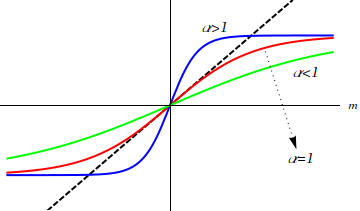
\includegraphics[width=250pt,keepaspectratio=true]{Addons/autocons.png}
\caption{\footnotesize{Plot dell'equazione di autoconsistenza $m=\tanh(\alpha m)$ per $\alpha>1,\alpha<1,\alpha=1$.}}
\end{figure}

Notiamo immediatamente che per $\beta Jz<1$, esiste una sola soluzione dell'equazione di autoconsistenza, cioè $m=0$, mentre per $\beta Jz>1$ vi sono tre soluzioni, $m=0, \pm m(\beta)$. Questa osservazione ci permette di definire un valore critico della temperatura $\beta_c=(Jz)^{-1}$, cioè $kT_c=Jz$ tale che per $T>T_c$ si abbia la sola soluzione $m=0$ (fase paramagnetica), mentre per $T<T_c$ si abbiano tre soluzioni $m=0,\pm m(T)$ (fase ferromagnetica). \\
Calcoliamo adesso la suscettività magnetica per $T>T_c$:
\begin{align*}
\chi(T) &= N\left.\dev{m}{h}\right|_{h=0}=N\left.\frac{\diff}{\diff{h}}\tanh[\beta(Jzm+h)]\right|_{h=0}\simeq N\left.\frac{\diff}{\diff{h}}[\beta Jzm+\beta h]\right|_{h=0} \\
&=\beta Jz N\left.\dev{m}{h}\right|_{h=0}+N\beta=\frac{\beta}{\beta_c}\chi+N\beta\;,
\end{align*}
da cui:
\begin{equation}
\boxed{\chi(T>T_c)=\frac{N\beta}{1-\beta/\beta_c}=\frac{N}{k(T-T_c)}}\;.
\end{equation}
La suscettività diverge per $T\to T_c$, cioè vicino alla transizione di fase basta una piccola variazione del campo magnetico per ottenere una grande variazione della magnetizzazione. \\
Studiamo quindi com'è fatta l'energia libera vicino al punto di transizione. Sia in fase ferromagnetica che in fase paramagnetica, per $h=0$, $m(h)\ll 1$. Possiamo sviluppare quindi l'energia libera per $m\to 0$:
\begin{align}
F(T,h=0,m) &= NJz\frac{m^2}{2}-NkT\ln[\cosh(\beta Jzm)]-NkT\ln 2 \notag \\
&\simeq NJz\left[\frac{m^2}{2}-\frac{kT}{Jz}\left(\frac{(\beta Jzm)^2}{2}-\frac{(\beta Jzm)^4}{12}\right)\right]+\mathcal{O}(m^6) \notag \\
&= NJz\left[\frac{m^2}{2}\left(1-\frac{\beta}{\beta_c}\right)+\left(\frac{\beta}{\beta_c}\right)^3\frac{m^4}{12}+\cdots\right] \notag \\
&\simeq  NJz\left[\left(\frac{T}{T_c}-1\right)\frac{m^2}{2}+\frac{m^4}{12}\right]+\mathcal{O}(m^6)\;. \label{ch4_landaufreeenergy}
\end{align}
Questa è la forma dell'\emph{energia libera di Landau}, che è tipica di qualunque fenomeno in cui avvenga rottura spontanea di simmetria.

\begin{center}
\begingroup
  \makeatletter
  \providecommand\color[2][]{%
    \GenericError{(gnuplot) \space\space\space\@spaces}{%
      Package color not loaded in conjunction with
      terminal option `colourtext'%
    }{See the gnuplot documentation for explanation.%
    }{Either use 'blacktext' in gnuplot or load the package
      color.sty in LaTeX.}%
    \renewcommand\color[2][]{}%
  }%
  \providecommand\includegraphics[2][]{%
    \GenericError{(gnuplot) \space\space\space\@spaces}{%
      Package graphicx or graphics not loaded%
    }{See the gnuplot documentation for explanation.%
    }{The gnuplot epslatex terminal needs graphicx.sty or graphics.sty.}%
    \renewcommand\includegraphics[2][]{}%
  }%
  \providecommand\rotatebox[2]{#2}%
  \@ifundefined{ifGPcolor}{%
    \newif\ifGPcolor
    \GPcolorfalse
  }{}%
  \@ifundefined{ifGPblacktext}{%
    \newif\ifGPblacktext
    \GPblacktexttrue
  }{}%
  % define a \g@addto@macro without @ in the name:
  \let\gplgaddtomacro\g@addto@macro
  % define empty templates for all commands taking text:
  \gdef\gplbacktext{}%
  \gdef\gplfronttext{}%
  \makeatother
  \ifGPblacktext
    % no textcolor at all
    \def\colorrgb#1{}%
    \def\colorgray#1{}%
  \else
    % gray or color?
    \ifGPcolor
      \def\colorrgb#1{\color[rgb]{#1}}%
      \def\colorgray#1{\color[gray]{#1}}%
      \expandafter\def\csname LTw\endcsname{\color{white}}%
      \expandafter\def\csname LTb\endcsname{\color{black}}%
      \expandafter\def\csname LTa\endcsname{\color{black}}%
      \expandafter\def\csname LT0\endcsname{\color[rgb]{1,0,0}}%
      \expandafter\def\csname LT1\endcsname{\color[rgb]{0,1,0}}%
      \expandafter\def\csname LT2\endcsname{\color[rgb]{0,0,1}}%
      \expandafter\def\csname LT3\endcsname{\color[rgb]{1,0,1}}%
      \expandafter\def\csname LT4\endcsname{\color[rgb]{0,1,1}}%
      \expandafter\def\csname LT5\endcsname{\color[rgb]{1,1,0}}%
      \expandafter\def\csname LT6\endcsname{\color[rgb]{0,0,0}}%
      \expandafter\def\csname LT7\endcsname{\color[rgb]{1,0.3,0}}%
      \expandafter\def\csname LT8\endcsname{\color[rgb]{0.5,0.5,0.5}}%
    \else
      % gray
      \def\colorrgb#1{\color{black}}%
      \def\colorgray#1{\color[gray]{#1}}%
      \expandafter\def\csname LTw\endcsname{\color{white}}%
      \expandafter\def\csname LTb\endcsname{\color{black}}%
      \expandafter\def\csname LTa\endcsname{\color{black}}%
      \expandafter\def\csname LT0\endcsname{\color{black}}%
      \expandafter\def\csname LT1\endcsname{\color{black}}%
      \expandafter\def\csname LT2\endcsname{\color{black}}%
      \expandafter\def\csname LT3\endcsname{\color{black}}%
      \expandafter\def\csname LT4\endcsname{\color{black}}%
      \expandafter\def\csname LT5\endcsname{\color{black}}%
      \expandafter\def\csname LT6\endcsname{\color{black}}%
      \expandafter\def\csname LT7\endcsname{\color{black}}%
      \expandafter\def\csname LT8\endcsname{\color{black}}%
    \fi
  \fi
    \setlength{\unitlength}{0.0500bp}%
    \ifx\gptboxheight\undefined%
      \newlength{\gptboxheight}%
      \newlength{\gptboxwidth}%
      \newsavebox{\gptboxtext}%
    \fi%
    \setlength{\fboxrule}{0.5pt}%
    \setlength{\fboxsep}{1pt}%
\begin{picture}(7200.00,5040.00)%
    \gplgaddtomacro\gplbacktext{%
      \csname LTb\endcsname%
      \put(550,1706){\makebox(0,0)[r]{\strut{}$0$}}%
      \put(2417,484){\makebox(0,0){\strut{}$-m(T)$}}%
      \put(5068,484){\makebox(0,0){\strut{}$m(T)$}}%
      \put(3743,484){\makebox(0,0){\strut{}$0$}}%
    }%
    \gplgaddtomacro\gplfronttext{%
      \csname LTb\endcsname%
      \put(176,2541){\rotatebox{-270}{\makebox(0,0){\strut{}$F(m,0,T)$}}}%
      \put(3742,154){\makebox(0,0){\strut{}$m$}}%
      \put(3742,4709){\makebox(0,0){\strut{}Landau free energy}}%
      \csname LTb\endcsname%
      \put(1342,1317){\makebox(0,0)[r]{\strut{}$T=T_c$}}%
      \csname LTb\endcsname%
      \put(1342,1097){\makebox(0,0)[r]{\strut{}$T>T_c$}}%
      \csname LTb\endcsname%
      \put(1342,877){\makebox(0,0)[r]{\strut{}$T<T_c$}}%
    }%
    
    \gplbacktext
    \put(0,0){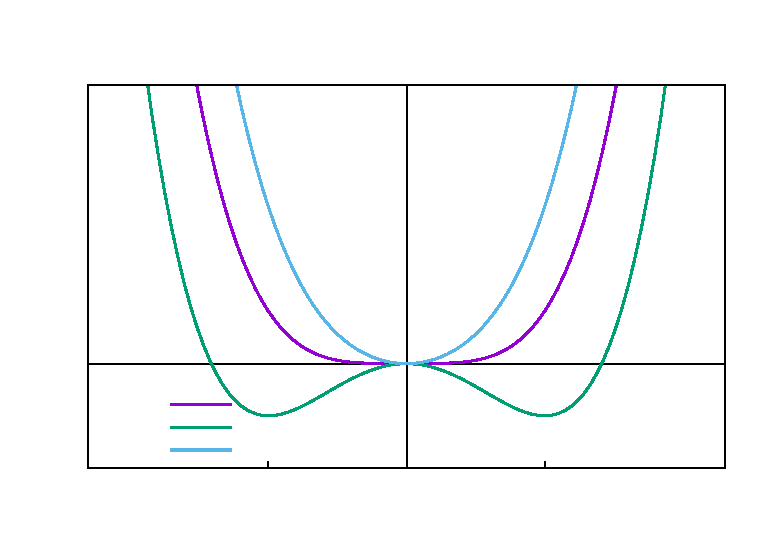
\includegraphics{Addons/landaufree}}%
    \gplfronttext
  \end{picture}%
\endgroup
\end{center}

Per $T<T_c$, $m=0$ è una soluzione instabile (massimo locale), mentre $\pm m(T)$ sono soluzioni stabili degeneri. Il sistema sceglie spontaneamente uno dei due minimi (rottura spontanea di simmetria). Minimizzando $F$ troviamo:
\begin{equation}
\pdev{F}{m}=0=NJz\left[m\left(\frac{T}{T_c}-1\right)+\frac{m^3}{3}\right]\qquad \Longrightarrow \qquad m=\begin{cases}
0\qquad T>T_c\;, \\
\\
\pm \sqrt{3\left(1-\dfrac{T}{T_c}\right)}\qquad T<T_c\;.
\end{cases}
\end{equation}
Calcoliamo le varie quantità termodinamiche vicino alla transizione.
\begin{itemize}
\item Energia libera.
\begin{equation}
F+NkT\ln 2=\begin{cases}
0\qquad T>T_c\;, \\
\\
-\dfrac{3}{4}NJz\tau^2\qquad T<T_c\;,
\end{cases}
\end{equation}
dove $\tau\equiv 1-T/T_c$.
\item Entropia.
\begin{equation}
S(T)=-\pdev{F}{T}=Nk\ln 2-\frac{3Nk}{2}\tau \theta(T_c-T)\;.
\end{equation}
\item Capacità termica.
\begin{equation}
\frac{C}{T}=\pdev{S}{T}=\frac{3Nk}{2T_c}\theta(T_c-T)\;.
\end{equation}
\end{itemize}
Notiamo che $F$ e $S$ sono continue, mentre $C=T\partial^2F/\partial T^2$ è discontinua, dunque si tratta di una transizione di fase del secondo ordine. \\
\\
Consideriamo adesso $h\ne 0$. La simmetria si rompe: il caso con $m$ parallelo ad $h$ sarà favorito rispetto al caso antiparallelo. I due minimi degeneri non lo sono più. \\
Nel caso $h=0$, sviluppando $F$ per $m$ piccolo, ottenevamo l'espressione \eqref{ch4_landaufreeenergy}, invariante per $m\to -m$. Se adesso sviluppiamo l'energia libera per $m,h$ piccoli, otteniamo la seguente forma:
\begin{equation}
F\simeq \left(\frac{T}{T_c}-1\right)\frac{m^2}{2}+\frac{m^4}{12}-hm+\mathrm{cost}(h)m^3\;,
\end{equation}
che non è più invariante per $m\to -m$. \\

Per $T<T_c$ abbiamo sempre tre stati stazionari, di cui un massimo e due minimi inequivalenti (un minimo è stabile e l'altro è metastabile.

\begin{figure}[h]
\centering
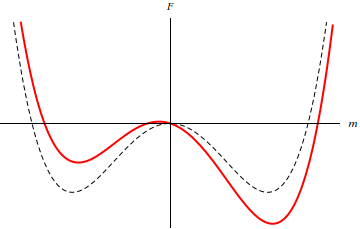
\includegraphics[width=250pt,keepaspectratio=true]{Addons/fhnotzero.png}
\caption{\footnotesize{Energia libera di Landau per $T<T_c$ nel caso $h=0$ (tratteggiato) e $h>0$ (rosso).}}

\end{figure}

Per $T>T_c$ si ha un solo minimo stabile $m(T)\ne 0$, con $m(T)\gtrless 0$ se $h\gtrless 0$.

\begin{figure}[h]
\centering
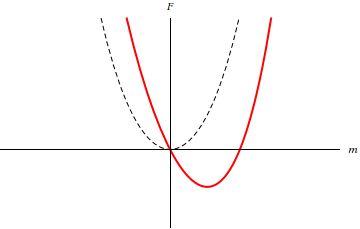
\includegraphics[width=250pt,keepaspectratio=true]{Addons/para.png}
\caption{Energia libera di Landau per $T>T_c$ nel caso $h=0$ (tratteggiato) e $h>0$ (rosso).}

\end{figure}

Per $T\ge T_c$ e per ogni valore del campo magnetico, $m(T,h)$ è \emph{single valued}, mentre per $T<T_c$ è \emph{triple valued}. L'esistenza del minimo metastabile è legata al fenomeno dell'isteresi.\\
Notiamo che per $T<T_c$, $m$ ha una discontinuità che vale $2m(T)$ in $h=0$; essendo $m=\partial F/\partial h$, concludiamo che se $h\ne 0$ abbiamo una transizione di fase del primo ordine, che diventa del secondo ordine per $h=0$.

\subsection{Campo medio in teoria di campo}
Cerchiamo di ricavare l'equazione di campo medio in un modo alternativo. Usiamo due strumenti matematici.

\begin{itemize}
\item \textbf{Trasformazione di Hubbard-Stratonovic}. Partiamo dall'osservare che, se $a>0$,
$$
\int_{-\infty}^{+\infty}\diff{\phi}\; e^{-\phi^2/2a+s\phi}=e^{as^2/2}\sqrt{2\pi a}\;.
$$
Estendendo a più variabili, sia $A$ una matrice simmetrica $N\times N$ definita positiva, allora:
\begin{equation}
\int_{-\infty}^{+\infty}\left(\prod_i\diff{\phi_i}\right)\exp\left[-\frac{1}{2}\sum_{i,j}\phi_i\left(A^{-1}\right)_{ij}\phi_j+\sum_is_i\phi_i\right]=(2\pi)^{N/2}\sqrt{\det A}\exp\left[\frac{1}{2}\sum_{i,j}s_iA_{ij}s_j\right]\;,
\end{equation}
con $i,j=1,\ldots,N$.
\item \textbf{Metodo di punto sella.} Sia:
$$
I=\int_a^b e^{Ng(x)}\;\diff{x}\;,
$$
con $N\gg 1$ e $g(x)$ funzione che abbia un solo massimo $\overline{x}\in [a,b]$. Espandendo intorno a $\overline{x}$:
$$
g(x)=g(\overline{x})+\underbrace{g'(\overline{x})}_{=0}(x-\overline{x})+\frac{1}{2}\underbrace{g''(\overline{x})}_{<0}(x-\overline{x})^2+\cdots\;.
$$
Allora:
\begin{align}
I &\simeq e^{Ng(\overline{x})}\int_a^b\diff{x}\; e^{-N|g''(\overline{x})|(x-\overline{x})^2/2} \notag \\
&\simeq e^{Ng(\overline{x})}\int_{-\infty}^{+\infty}\diff{x}\;e^{-N|g''(\overline{x})|(x-\overline{x})^2/2} \notag \\
&= e^{Ng(\overline{x})}\left(\frac{2\pi}{N|g''(\overline{x})|}\right)^{1/2}\;, \\
\ln I &\simeq Ng(\overline{x})+\mathcal{O}(\ln N)\;.
\end{align}
\end{itemize}

La funzione di partizione del modello di Ising può quindi  essere riscritta introducendo un campo ausiliario $\phi_i$:
\begin{align}
\zpart &= \sum_{\{s_i\}}e^{-\frac{\beta}{2}\sum_{i,j}J_{ij}s_is_j+\beta\sum_is_ih_i} \notag \\
&= \frac{1}{(2\pi kT)^{N/2}\sqrt{\det J}}\int_{-\infty}^{+\infty}\left(\prod_{i'}\diff{\phi_{i'}}\right)e^{\frac{\beta}{2}\sum_{i,j}(J^{-1})_{ij}(\phi_i-h_i)(\phi_j-h_j)}\prod_i\sum_{s_i=\pm 1}e^{\beta\phi_is_i} \notag \\
&= \frac{1}{(2\pi kT)^{N/2}\sqrt{\det J}}\int_{-\infty}^{+\infty}\left(\prod_{i'}\diff{\phi_{i'}}\right)e^{\frac{\beta}{2}\sum_{i,j}(J^{-1})_{ij}(\phi_i-h_i)(\phi_j-h_j)+\sum_i\ln[2\cosh(\beta \phi_i)]}\;,
\end{align}
dove abbiamo usato la matrice $N\times N$:
\begin{equation}
J_{ij}=\begin{cases}
-J,\qquad \mbox{se}\; i,j\;\mbox{primi vicini}\;, \\
\\
0,\qquad \mbox{altrimenti}\;.
\end{cases}
\end{equation}
Notiamo che possiamo scrivere:
$$
\zpart=C\int_{-\infty}^{+\infty}\left(\prod_i\diff{\phi_i}\right)e^{-\beta S(\phi_i,h_i)}=e^{\beta F}\;,
$$
dove $C=1/[(2\pi kT)^{N/2}\sqrt{\det J}]$ e :
\begin{equation}
S(\phi_i,h_i)=-\frac{1}{2}\sum_{i,j}(J^{-1})_{ij}(\phi_i-h_i)(\phi_j-h_j)-\frac{1}{\beta}\sum_i\ln[2\cosh(\beta \phi_i)]\;,
\end{equation}
e una sorta di azione in teoria di campo. Usiamo quindi l'approssimazione di punto sella:
$$
\zpart\simeq Ce^{-\beta S(\overline{\phi}_i,h_i)}\;.
$$
$\overline{\phi}_i$ è determinato da:
\begin{align*}
\left.\pdev{S}{\phi_i}\right|_{\phi=\overline{\phi}_i}&=-\sum_j(J^{-1})_{ij}\overline{\phi}_j-h_j)-\tanh(\beta\overline{\phi}_i)=0\;,
\overline{\phi}_i-h_i &= \sum_j J_{ij}\tanh(\beta\overline{\phi}_j)\;.
\end{align*}
Se $h_i=0$ per ogni $i$, allora la soluzione $\overline{\phi}_i$ deve essere uniforme, cioè $\overline{\phi}_i\equiv\overline{\phi}$ per ogni $i$ e deve essere tale che:
\begin{equation}
\overline{\phi}=-\sum_jJ_{ij}\tanh(\beta\overline{\phi})=Jz\tanh(\beta\overline{\phi})\;,
\end{equation}
in quanto contribuiscono solo i primi vicini. Possiamo quindi calcolare la magnetizzazione:
\begin{align}
m &=\bra s_i\ket =kT\left.\pdev{\ln\zpart}{h_i}\right|_{h_i=0}=-\left.\dev{S(\overline{\phi}_i,h_i)}{h_i}\right|_{h_i=0} \notag \\
&=-\sum_j(J^{-1})_{ij}\overline{\phi}_j=\tanh(\beta\overline{\phi})\;.
\end{align}
Mettendo insieme quindi le due equazioni che abbiamo trovato:
\begin{align*}
m &= \tanh(\beta\overline{\phi})\;, \\
\overline{\phi} &= Jz\tanh(\beta\overline{\phi})\;,
\end{align*}
otteniamo infine:
\begin{equation}
m=\frac{\overline{\phi}}{Jz}\;.
\end{equation}
\subsection{Funzione di correlazione e suscettività}
La funzione di correlazione è definita come:
\begin{equation}
\Gamma_{ij}=\bra s_is_j\ket-\bra s_i\ket\bra s_j\ket=(kT)^2\left.\frac{\partial^2\ln\zpart}{\partial h_i\partial h_j}\right|_{h_i=0}=-kT\left.\frac{\diff^2{S(\overline{\phi}_i,h_i)}}{\diff{h_i}\diff{h_j}}\right|_{h_j=0}\;.
\end{equation}
$\Gamma_{ij}$ è invariante per traslazioni, quindi $\Gamma_{ij}=\Gamma(\mathbf{r}_i-\mathbf{r}_j)$. Possiamo quindi definire una trasformata di Fourier come:
\begin{equation}
\Gamma(\mathbf{q})=\sum_{\mathbf{r}_i-\mathbf{r}_j}\Gamma(\mathbf{r}_i-\mathbf{r}_j)e^{-i\mathbf{q}\cdot(\mathbf{r}_i-\mathbf{r}_j)}=\sum_j\Gamma_{ij}e^{-i\mathbf{q}\cdot(\mathbf{r}_i-\mathbf{r}_j)}\;.
\end{equation}
In generale, se:
$$
b_i=\sum_j \Gamma_{ij}a_j\qquad \Longleftrightarrow\qquad a_i=\sum_j(\Gamma^{-1})_{ij}b_j\;,
$$
si ha:
\begin{align*}
b(\mathbf{q})&=\sum_ib_ie^{-i\mathbf{q}\cdot\mathbf{r}_i}=\sum_{i,j}\Gamma_{ij}a_je^{-i\mathbf{q}\cdot\mathbf{r}_i} \\
&=\sum_{i,j}\Gamma_{ij}a_je^{-i\mathbf{q}\cdot(\mathbf{r}_i-\mathbf{r}_j)}e^{-i\mathbf{q}\cdot\mathbf{r}_i} \\
&=\sum_i\Gamma_{ij}e^{-i\mathbf{q}\cdot(\mathbf{r}_i-\mathbf{r}_j)}\sum_ja_je^{-i\mathbf{q}\cdot\mathbf{r}_j}=\Gamma(\mathbf{q})a(\mathbf{q})\;.
\end{align*}
e l'inversa $a(\mathbf{q})=\Gamma^{-1}(\mathbf{q})b(\mathbf{q})$. Confrontando si ottiene $\Gamma^{-1}(\mathbf{q})=\dfrac{1}{\Gamma(\mathbf{q})}$. Possiamo quindi scrivere ($d$ è il numero di dimensioni del sistema):
\begin{equation}
\Gamma(\mathbf{q})=\sum_j\Gamma_{ij}e^{-i\mathbf{q}\cdot(\mathbf{r}_i-\mathbf{r}_j)}=\frac{1}{N}\sum_{i,j}\Gamma_{ij}e^{-i\mathbf{q}\cdot(\mathbf{r}_i-\mathbf{r}_j)}\;,
\end{equation}
e:
\begin{equation}
\Gamma_{ij}=\int_{BZ}\frac{\diff^d{q}}{(2\pi)^d}\Gamma(\mathbf{q})e^{i\mathbf{q}(\mathbf{r}_i-\mathbf{r}_j)}\;,
\end{equation}
dove $BZ$ indica la zona di Brillounain. Useremo anche:
\begin{align}
\delta_{ij} &= \int\frac{\diff^d{q}}{(2\pi)^d}e^{i\mathbf{q}\cdot(\mathbf{r}_i-\mathbf{r}_j)}\;, \label{ch5_deltaaij} \\
J_{ij} &=\int\frac{\diff^d{q}}{(2\pi)^d}J(\mathbf{q})e^{i\mathbf{q}\cdot(\mathbf{r}_i-\mathbf{r}_j)}\;. \label{ch5_jij}
\end{align}
Sapendo che:
$$
m=\bra s_i\ket=-\dev{S(\phi_i,h_i)}{h_j}=\tanh(\beta\phi_i)\;,
$$
possiamo scrivere:
\begin{equation}
\beta\Gamma_{ij}=-\left.\dev{\bra s_i\ket}{h_j}\right|_{h_j=0}=-\left.\frac{\diff}{\diff{h_j}}\tanh(\beta\overline{\phi}_i)\right|_{h_j=0}=\frac{\beta}{\cosh^2(\beta\overline{\phi})}\left.\dev{\overline{\phi}_i}{h_j}\right|_{h_j=0}\;.
\end{equation}
Dall'equazione di punto sella:
$$
h_j=\overline{\phi}_j+\sum_{j'}J_{jj'}\tanh(\beta\overline{\phi}_{j'})\;,
$$
ricaviamo:
\begin{equation}
\dev{h_j}{\overline{\phi}_i}=\delta_{ij}+\beta J_{ij}\frac{1}{\cosh^2(\beta\overline{\phi}_i)}\;.
\end{equation}
Invertendo la \eqref{ch5_deltaaij} e usando la \eqref{ch5_deltaij} otteniamo:
\begin{equation}
(\Gamma^{-1})_{ij}=\cosh^2(\beta\overline{\phi})\left.\dev{h_j}{\overline{\phi}_i}\right|_{h_j=0}=\cosh^2(\beta\overline{\phi})\left[\delta_{ij}+\frac{\beta J_{ij}}{\cosh^2(\beta\overline{\phi})}\right]\;.
\end{equation}
Trasformiamo quest'ultima espressione con Fourier:
$$
\frac{1}{\Gamma(\mathbf{q})}=\cosh^2(\beta\overline{\phi})+\beta J(\overline{q})\;,
$$
e quindi:
\begin{equation}
\Gamma(\mathbf{q}) =\frac{1}{\cosh^2(\beta\overline{\phi})+\beta J(\mathbf{q})}=\frac{1/\cosh^2(\beta\overline{\phi})}{1+\dfrac{\beta}{\cosh^2(\beta\overline{\phi})J(\mathbf{q})}}=\frac{\Gamma_0/\beta}{1+\Gamma_0J(\mathbf{q})}\;,
\end{equation}
dove:
\begin{equation}
\Gamma_0=\frac{\beta}{\cosh^2(\beta\overline{\phi})}=\beta(1-\tanh^2(\beta\overline{\phi})=\beta(1-m^2)\;,
\end{equation}
per l'equazioni di autoconsistenza. $J(\mathbf{q})$ contiene tutte le informazioni sul reticolo. Valutiamo questa quantità per un reticolo $d$-dimensionale ipercubico. Dalla definizione:
$$
J(\mathbf{q})=\frac{1}{N}\sum_{i,j}J_{ij}e^{i\mathbf{q}\cdot(\mathbf{r}_i-\mathbf{r}_j)}\;.
$$
$J_{ij}$ è non nullo solo se $|\mathbf{r}_i-\mathbf{r}_j|=a$, passo reticolare:
\begin{equation}
J(\mathbf{q})=-J\sum_{\alpha=1}^d(e^{iq_{\alpha}a}+e^{-iq_{\alpha}a})=-2J\sum_{\alpha=1}^d\cos(q_{\alpha}a)\;.
\end{equation}
Per piccoli $q\equiv |\mathbf{q}|$, cioè $qa\ll 1$ si ha:
\begin{equation}
J(\mathbf{q})\simeq -J\underbrace{(2d)}_{z}+J\sum_{\alpha=1}^d q_{\alpha}^2a^2+o(q^4)=-Jz+Jq^2a^2+o(q^4)\;.
\end{equation}
Questa espansione è vera in generale, a patto di definire bene $a$. Per $\Gamma(\mathbf{q})$ invece lo sviluppo porta a 
\begin{equation}
\Gamma(\mathbf{q})=\frac{kT}{\dfrac{1}{\Gamma_0}+J(\mathbf{q})}\simeq \frac{kT}{\dfrac{kT}{1-m^2}-\underbrace{Jz}_{kT_c}+Jq^2a^2+o(q^4)}\;.
\end{equation}
Per $T\simeq T_c$, $m^2\ll 1$, quindi:
$$
\Gamma(\mathbf{q})=\frac{kT}{k(T-T_c)+Jq^2a^2+kTm^2+o(q^4,m^4)}=\frac{kT}{k(T-T_c)+kTm^2}\frac{1}{1+\dfrac{Ja^2}{k(T-T_c)+kTm^2}q^2+o(q^4,m^4)}\;.
$$
$\Gamma(\mathbf{q})$ assume una forma universale, detta \emph{forma di Orstein-Zernike}:
\begin{equation}
\Gamma(\mathbf{q})=\frac{\mathrm{const}}{1+q^2\xi^2}\;,
\end{equation}
dove $\xi$ è detta \emph{lunghezza di correlazione} (assume valori diversi a seconda che $T\lessgtr T_c$):
\begin{itemize}
\item se $T>T_c$, allora $m=0$ e:
\begin{equation}
\xi^2=\frac{Ja^2}{k(T-T_c)}\;,
\end{equation}
che diverge per $T\to T_c$;
\item se $T<T_c$ allora:
\begin{equation}
\xi^2=\frac{Ja^2}{k(T-T_c)+kTm^2}\;,
\end{equation}
per $T\to T_c$ $m^2\simeq 3(T_c-T)/T$, quindi:
\begin{equation}
\xi^2\simeq \frac{Ja^2}{2k|T-T_c|}\;,
\end{equation}
e anche questa forma diverge per $T=T_c$.
\end{itemize}
La funzione di correlazione si scrive allora come:
\begin{equation}
\Gamma_{\mathbf{r}}=\int\frac{\diff^d{q}}{(2\pi)^d}\Gamma(\mathbf{q})e^{i\mathbf{q}\cdot\mathbf{r}}=\int\frac{\diff^d{q}}{(2\pi)^d}\frac{\mathrm{const}}{1+q^2\xi^2}e^{i\mathbf{q}\cdot\mathbf{r}}\propto \frac{e^{-|\mathbf{r}|/\xi}}{r^{(d-1)/2}}\;.
\end{equation}
$\xi$ rappresenta quindi la distanza tipica in cui il sistema è correlato. Alla temperatura critica, $\xi\to\infty$, $\Gamma(\mathbf{q})\sim 1/q^2$ e:
$$
\Gamma_{\mathbf{r}}\propto\int \diff^d{q}\;\frac{e^{i\mathbf{q}\cdot\mathbf{r}}}{q^2}=\begin{cases}
\dfrac{1}{r^{d-2}},\qquad d>2\;, \\
\\
\ln r,\qquad d=2\;.
\end{cases}
$$
Il caso $d=2$ è una patologia del campo medio, quindi non lo considereremo mai. Nel limite $r\to\infty$, $\Gamma_{\mathbf{r}}\to 0$ e quindi:
$$
\bra s_is_j\ket-\bra s_i\ket\bra s_j\ket=0\qquad \Longrightarrow\qquad \bra s_is_j\ket=m^2\;,
$$
da cui emerge un ordine a lungo raggio del sistema.
\subsection{Suscettività}
La suscettività è data da:
$$
\chi=N\left.\dev{m}{h}\right|_{h=0}\;.
$$
Nel caso specifico si ha:
\begin{align}
\chi &=\beta\sum_{i,j}(\bra s_is_j\ket-\bra s_i\ket\bra s_j\ket)=\beta\sum_{i,j}\Gamma_{ij}=N\beta\Gamma(\mathbf{q}=0) \notag \\
&=\frac{N}{k(T-T_c)+kTm^2}=\begin{cases}
\dfrac{N}{k(T-T_c)}\qquad T>T_c\;, \\
\\
\dfrac{N}{2k|T-T_c|}\qquad T<T_c\;.
\end{cases}
\end{align}
Notiamo che la suscettività diverge a $T=T_c$ per entrambe le fasi.
\section{Teoria di Landau-Ginzburg}
Questa teoria si basa sull'espressione di Landau per l'energia libera, $F=Am^2+Bm^4-hm$, che viene assunta come tipica per le transizioni di fase del secondo ordine. \\
L'idea di Landau si fonda sulla simmetria del sistema e sul fenomeno della rottura spontanea di simmetria:
\begin{itemize}
\item la fase di alta temperatura è caratterizzata da un certo gruppo di simmetria $G$, le cui trasformazioni lasciano il sistema invariato (nel caso del modello di Ising, l'inversione degli spin);
\item la fase di bassa temperatura ha invece un gruppo di simmetria $G'\subset G$ dovuto all'apparizione di un ordine (Ising: ordine ferromagnetico).
\end{itemize}
La "riduzione" di simmetria è accompagnata dall'apparire di un parametro d'ordine che non possiede tutte le simmetrie di $G$. Nel caso del modello di Ising, il parametro d'ordine è la magnetizzazione $m$. Il gruppo di simmetria è $\mathbb{Z}_2=\{I,P\}$ (identità + inversione degli spin), per cui $m$ non è infatti invariante.
\subsection{Teoria di Landau-Ginzburg per il modello di Ising}
Introduciamo innanzitutto il concetto di \emph{coarse-graining}. Consideriamo nel reticolo una celletta $d-$dimensionale di lato $L_d$ contenente $N_b$ spin. La regione è centrata nel sito $\mathbf{r}_i$ e la indichiam con $\Lambda_b(\mathbf{r})$. Definiamo a questo punto:
\begin{equation}
m(\mathbf{r})\equiv \frac{1}{N_b}\sum_{i\in\Lambda_b(\mathbf{r})}\bra s_i\ket\;.
\end{equation}
Per $N_b$ molto grande, la funzione $m(\mathbf{r})$ è continua. L'energia libera di Landau-Ginzburg si scrive allora come
\begin{equation}
F(m(\mathbf{r}),h,T)=F_0(h,T)+\int\diff^d{r}\left[\frac{A}{2}m^2(\mathbf{r})+\frac{B}{4}m^4(\mathbf{r})-h(\mathbf{r})m(\mathbf{r})+\frac{k}{2}(\nabla m(\mathbf{r}))^2\right]\;,
\end{equation}
dove il termine in $k$ tiene conto delle fluttuazioni di $m(\mathbf{r})$ e:
\begin{align*}
A &= \frac{Jz}{a^d}\left(\frac{T}{T_c}-1\right)\;, \\
B &= \frac{Jz}{3a^d}\;.
\end{align*}
\subsection*{Giustificazione e calcolo di $k$}
Cerchiamo di minimizzare $F$ rispetto a $m$. Questa volta però si tratta di una derivata funzionale:
\begin{equation}
0=\frac{\delta F}{\delta m}=\pdev{F}{m}-\nabla\cdot\pdev{F}{\nabla m}=-k\nabla^2m+Am+Bm^3-h\;. \label{ch5_landaufreeen2}
\end{equation}
Confrontiamo questa con l'equazione di punto sella:
$$
\overline{\phi}_i=h_i-\sum_j J_{ij}\tanh(\beta\overline{\phi}_j)\;,
$$
in cui $h_i=0$ e scriviamo $\overline{\phi}_i\equiv \overline{\phi}(\mathbf{r}_i)$. Quindi, vicino alla temperatura critica, si ha:
$$
\overline{\phi}(\mathbf{r}_i)\simeq -\beta\sum_j J_{ij}\overline{\phi}(\mathbf{r}_j)=\beta J\sum_{\mathbf{a}\; n.n.\mathbf{r}_i}\overline{\phi}(\mathbf{r}_i+\mathbf{a})\;,
$$
dove la sommatoria è estesa sugli $\mathbf{a}$ primi vicini (nearest neighbor) ad $\mathbf{r}_i$. Espandiamo adesso in $\mathbf{a}$:
$$
\overline{\phi}(\mathbf{r}_i)\simeq \beta J\left[z\overline{\phi}(\mathbf{r}_i)+\sum_{\mathbf{a}\; n.n.\mathbf{r}_i}\mathbf{a}\cdot \nabla\overline{\phi}(\mathbf{r}_i)+\frac{1}{2}\sum_{\mathbf{a}\; n.n.\mathbf{r}_i}\sum_{\mu,\nu}a_{\mu}a_{\nu}\frac{\partial^2}{\partial r_{\mu}\partial r_{\nu}}\overline{\phi}(\mathbf{r}_i)+\cdots\right]\;,
$$
con $\mu,\nu=\{x,y,z\}$. Il primo termine è nullo (si sommano contributi opposti), mentre nel secondo sopravvivono solo quelli con $\mu=\nu$. Combinando questi fatti con l'equazione di autoconsistenza $\overline{\phi}(\mathbf{r}_i)=Jzm(\mathbf{r}_i)$ troviamo:
\begin{align}
Jzm(\mathbf{r}) &= \beta J\left[zJzm(\mathbf{r})+\frac{1}{2}Jz2a^2\nabla^2m(\mathbf{r})\right] \notag \\
&m(\mathbf{r})\left(1-\frac{\beta}{\beta_c}\right)-\beta Ja^2\nabla^2m(\mathbf{r})=0\;,
\end{align}
ricordando che $Jz=1/\beta_c$. Notiamo che questa equazione è identica alla forma di Landau \eqref{ch5_landaufreeen2}  (con $h=0$ e trascurando $m^3$). Dal confronto si ottiene dunque il valore di $k$ in prossimità della transizione:
\begin{equation}
k=Ja^{2-d}\;.
\end{equation}
L'equazione è spesso scritta come:
$$
-\nabla^2m+\frac{A}{k}m=0\;.
$$
Si vede che:
\begin{equation}
\frac{A}{k}=\frac{z(T/T_c-1)}{a^2}=\xi^{-2}\;,
\end{equation}
dove $\xi$ è la lunghezza di correlazione. Allora si ha:
\begin{equation}
m(\mathbf{r})-\xi^2\nabla^2m(\mathbf{r})=0\;.
\end{equation}
\section{Generalizzazioni del modello di Ising}
\begin{enumerate}
\item \textbf{Modello di Heisenberg}: in un ferromagnete, lo spin non punta in un'unica direzione. Lo scriviamo dunque in forma vettoriale $\mathbf{s}=(s_1,s_2,s_3)$ con $\mathbf{s}^2=1$. L'Hamiltoniana del modello di Heisenberg sarà dunque:
\begin{equation}
H=-J\sum_{\bra i,j\ket}\mathbf{s}_i\cdot\mathbf{s}_j-\sum_i\mathbf{h}\cdot\mathbf{s}_i\qquad\qquad \mbox{modello di Heisenberg}\;.
\end{equation}
\item \textbf{Modello xy}: in questo modello, lo spin ha due sole componenti, $\mathbf{s}=(s_1,s_2)$, $\mathbf{s}^2=1$. L'Hamiltoniana è identica a quella del modello di Heisenberg.
\item \textbf{Modello} $O(n)$: in questo modello, lo spin ha un numero arbitrario di componenti $\mathbf{s}=(s_1,\ldots,s_n)$ e l'Hamiltoniana è identica in forma a quella del modello di Heisenberg. Per $n=1$ questo coincide con il modello di Ising, per $n=2$ coincide con il modello $xy$ e per $n=3$ con quello di Heisenberg. Casi di particolare interesse sono $n=0$, che descrive il modello SAW (fisica dei polimeri) e $n=\infty$, che prende il nome di \emph{modello sferico}.
\end{enumerate}
Il gruppo di simmetria del modello è appunto $G=O(n)$, mentre dopo la rottura di simmetria diventa $G'=O(n-1)$.
\subsection{Teoria di Landau-Ginzburg per il modello $O(n)$}
L'energia libera è in generale data da:
\begin{equation}
F=\int\diff^d{r}\left[k(\nabla\mathbf{m})^2+A\mathbf{m}^2+B(\mathbf{m}^2)^2-\mathbf{h}\cdot\mathbf{m}\right]\;,
\end{equation}
dove:
$$
(\nabla\mathbf{m})^2=\sum_{i=1}^n\sum_{\mu=1}^d(\partial_{\mu}m_i)^2\;.
$$
Calcoliamo i coefficienti $A,B$ tramite la trasformazione di H-S: scriviamo la funzione di partizione:
\begin{equation}
\zpart=\sum_{\{\mathbf{s}_i\}}\exp\left(-\frac{\beta}{2}\sum_{i,j}J_{ij}\mathbf{s}_i\cdot\mathbf{s}_j+\beta\sum_i\mathbf{h}\cdot \mathbf{s}_i\right)\;.
\end{equation}
Introduciamo quindi gli $n$ campi $\boldsymbol{\phi}_i=(\phi_i^1,\ldots,\phi_1^n)$ e scriviamo:
\begin{equation}
\zpart= C\int_{-\infty}^{+\infty}\left(\prod_i\diff{\boldsymbol{\phi}_i}\right)\exp\left(\frac{\beta}{2}\sum_{i,j}(\boldsymbol{\phi}_i-\mathbf{h}_i)(J^{-1})_{ij}(\boldsymbol{\phi}_j-\mathbf{h}_j)\prod_i\sum_{\mathbf{s}_i}e^{\beta\boldsymbol{\phi}_i\cdot\mathbf{s}_i}\right)\;.
\end{equation}
L'unica differenza con il modello di Ising sta nell'ultima produttoria. Valutiamo quest'ultimo fattore per il modello $xy$:
\begin{equation}
\prod_i\sum_{\{\mathbf{s}_i\}}e^{\beta\boldsymbol{\phi}_i\cdot\mathbf{s}_i}=\prod_i\int_0^{2\pi}\diff{\theta_i}e^{\beta\phi_i\cos\theta_i}=\prod_i2\pi I_0(\beta\phi_i)\;,
\end{equation}
dove $I_0(\beta\phi)$ è la funzione di Bessel zero. Il nostro potenziale efficace sarà adesso $\ln(2\pi I_0(\beta\phi_i))$, che sviluppato in serie restituisce:
\begin{equation}
\ln(2\pi I_0(x))\simeq \ln(2\pi)+\frac{x^2}{4}-\frac{x^4}{64}\;.
\end{equation}
Usando questo sviluppo otteniamo:
\begin{equation}
F_{xy}=NJz\frac{\phi^2}{2}-NkT\ln(2\pi I_0(\beta\phi))=\frac{N\phi^2}{2}\left(Jz-\frac{\beta}{2}\right)+o(\phi^4)\;.
\end{equation}
La differenza con il modello di Ising è il fattore $1/2$ che compare prima di $\beta$. Questo porta a due temperature critiche differenti per i due modelli:
\begin{align*}
\beta_c^I= Jz\qquad &\Longrightarrow \qquad kT_c^I=\frac{1}{Jz}\;, \\
\beta_c^{xy}=2Jz\qquad &\Longrightarrow\qquad kT_c^{xy}=\frac{1}{2Jz}\;.
\end{align*}
Notiamo che $T^{xy}_c<T^I_c$, che riflette il fatto che è più facile disordinare una variabile continua (nel modello $xy$) rispetto a una discreta (Ising).
\section{Rottura spontanea di simmetria}
Si ha una rottura spontanea di simmetria quando, data un'Hamiltoniana $H[\phi]$ che dipende da certi gradi di libertà $\phi$ invariante per un certo gruppo di simmetria $G$, ossia $H[g\phi]=H[\phi]$ per ogni $g\in G$, lo stato fisico non è invariante sotto l'azione del gruppo $G$, dove per stato fisico intendiamo lo stato di Gibbs $e^{-\beta H}$ oppure lo stato fondamentale in Meccanica Quantistica. \\
Nella fase in cui la simmetria è rotta, gli stati fisici non sono invarianti, ma trasformano gli uni negli altri sotto l'azione di $G$. Inoltre, non tutte le simmetrie vengono rotte: si passa da una fase con gruppo di simmetria $G$ ad una con gruppo di simmetria $G'\subset G$, e gli stati fisici sono invarianti sotto l'azione del gruppo $G'$. Ad esempio, nel modello di Heisenberg si passa da $G=O(3)$ a $G'=O(2)$, ossia le rotazioni intorno all'asse della magnetizzazione.\\
La domanda adesso a cui vogliamo dare risposta è: perché nel calcolare lo stato di Gibbs $e^{-\beta H}$ i vari stati non entrano nella somma con lo stesso peso in modo tale che lo stato fisico sia simmetrico? Oppure, in termini quantistici, perché lo stato fondamentale non è una sovrapposizione di tutti questi stati? \\
Per rispondere, torniamo alla funzione di partizione delo modello di Ising in presenza di campo magnetico esterno $h$:
\begin{equation}
\zpart=\tr\;\exp\left[-\beta\left(H_i-h\sum_is_i\right)\right]\;.
\end{equation}
Questa non è invariante per $\mathbb{Z}_2$, però per un sistema finito $\lim_{h\to 0} \zpart$ è invariante per $\mathbb{Z}_2$ e questo porta ad una magnetizzazione $m$ nulla. Se adesso eseguiamo il limite termodinamico otteniamo che:
\begin{equation}
\lim_{N\to\infty}\lim_{h\to 0}\zpart\;,
\end{equation}
è invariante per $\mathbb{Z}_2$ e quindi ancora $m=0$. Apparentemente non dovremmo avere mai rottura spontanea. Tuttavia, se consideriamo invece:
\begin{equation}
\lim_{h\to 0}\lim_{N\to\infty}\zpart\;,
\end{equation}
questo \underline{potrebbe} portare ad un risultato diverso dal limite invertito. Il punto fondamentale è che un campo esterno, seppur piccolissimo, accoppia nel secondo caso infiniti spin. La differenza di energia tra due configurazioni di spin "simmetriche" è data da $\Delta E=2hN$, e chiaramente c'è differenza tra prendere il limite $h\to 0$ con $N$ finito e con $N$ infinito. Girare gli spin contro il campo potrebbe essere troppo costoso energicamente per essere battuto dalle fluttuazioni: in tal caso il sistema rimarrà in una configurazione che predilige una certa orientazione degli spin. \\
Quando ad essere rotta è una simmetria continua, abbiamo una conseguenza molto importante. Consideriamo l'Hamiltoniana di Landau-Ginzburg per il modello $O(n)$:
\begin{align}
H_{LG}[\vec{\phi}]&=\int\diff^d{r}\,\left[\frac{1}{2}(\partial_{\mu}\vec{\phi})^2+\frac{A}{2}(\vec{\phi})^2+\frac{B}{4}(\vec{\phi}^2)^2\right]\;, \\
\vec{\phi} &\equiv (\phi_1,\ldots,\phi_n)\;. \notag
\end{align}
Se $A<0$, abbiamo rottura spontanea, in cui $\vec{\phi}^2=-A/B$. Scegliamo come stato iniziale $\vec{\phi}_0=(0,0,\ldots,m)$ con $m=\sqrt{-A/B}$. Possiamo parametrizzare il campo $\vec{\phi}$ come:
\begin{equation}
\vec{\phi}=\vec{\pi}(x)+\hat{\mathbf{e}}_n\cdot(m+\sigma(x))\;,
\end{equation}
dove $\vec{\phi}$ è un campo con $n-1$ componenti, $\hat{\mathbf{e}}_n\equiv (0,0,0,\ldots, 1)$ e $\sigma$ sono le fluttuazioni della magnetizzazione $m$. Sostituendo nell'Hamiltoniana si trova:
\begin{equation}
H_{LG}=\int\diff^d{r}\left[\frac{1}{2}(\partial_{\mu}\vec{\pi})^2+\frac{1}{2}(\partial_{\mu}\sigma)^2+\frac{1}{2}(2A)\sigma^2+o(\sigma^3,\vec{\pi}^2\sigma^2,\vec{\pi}^4)\right]\;.
\end{equation}
Quello che si nota è che non c'è dipendenza quadratica dal campo $\vec{\phi}$, cioè manca il termine in $\vec{\pi}^2$ il cui coefficiente era proporzionale a $\xi^{-2}$, $\xi$ lunghezza di correlazione. Concludiamo che $\xi_{\pi}=\infty$ e quindi $\bra \pi_a(\mathbf{r})\pi_b(\mathbf{r}')\propto |\mathbf{r}-\mathbf{r}'|^{-\alpha}$, con $\alpha>0$. Queste $n-1$ componenti prendono il nome di \emph{modi soffici}. \\
Più in generale, si può dimostrare che se per un sistema abbiamo due gruppi di Lie $G,G'$, con $G'\subset G$, tali che $G$ abbia $n$ generatori e $G'$ abbia $m$ generatori $(m<n)$, allora esisteranno esattamente $n-m$ modi soffici.
\section{Esponenti critici}
Gli esponenti critici forniscono delle informazioni su come le quantità termodinamiche dipendano da $\tau=1-T/T_c$:
\begin{align*}
&\xi(T)\simeq |\tau|^{-\nu} & \mbox{lunghezza di correlazione}\;, \\
&\chi(T)\simeq |\tau|^{-\gamma} & \mbox{suscettività}\;, \\
&c_v(T)\simeq |\tau|^{-\alpha} &\mbox{calore specifico}\;, \\
&m(T)|_{T<T_c}\simeq (-\tau)^{\beta} & \mbox{magnetizzazione}\;, \\
&m(T=T_c,h)\simeq |h|^{1/\delta} & \mbox{magnetizzazione alla temperatura critica}\;, \\
&\Gamma_{\mathbf{r}}\simeq r^{-(d-2+\eta)} &\mbox{funzione di correlazione}\;.
\end{align*}
Le osservazioni sperimentali degli anni '60 suggerirono che gli esponenti critici non fossero indipendenti, bensì legati da \emph{leggi di scala}:
\begin{align}
&\alpha+2\beta+\gamma=2 &\mbox{formula di Rushbrooke}\;, \label{ch5_rushbrooke} \\
&\gamma=\beta(\delta-1) &\mbox{Widom scale}\;, \label{ch5_widom}\\
&\gamma=\nu(2-\eta) &\mbox{Fisher scale}\;, \label{ch5_fisher} \\
&\nu d=2-\alpha &\mbox{Josephson scale}\;. \label{josephson}
\end{align}
L'importanza degli esponenti critici risiede nella loro \underline{universalità}, cioè sistemi molto diversi con temperature critiche differenti anche per ordini di grandezza hanno gli stessi esponenti critici. Questa universalità emerge dalla teoria della normalizzazione, secondo cui i sistemi si dividono in classi di universalità caratterizzate da propri esponenti critici fissati. La classe di universalità è determinata dalla simmetria e dalla dimensionalità del sistema.
\subsection{Ipotesi di scaling}
Vicino al punto critico la lunghezza di correlazione $\xi$ è l'unica lunghezza caratteristica del sistema. Le altre lunghezze devono essere quindi misurate a partire da $\xi$. Partiamo da un'analisi dimensionale:
\begin{align*}
\left[\Gamma_{\mathbf{r}}\right]&=\left[\frac{1}{r^{d-2+\eta}}\right]=L^{2-d-\eta}\;, \\
[m] &= [\Gamma_{\mathbf{r}}^{1/2}]=L^{(2-d-\eta)/2}\;, \\
[\chi] &= \left[\int\diff^d{r}\;\Gamma_{\mathbf{r}}\right]=[\Gamma_{\mathbf{r}}]\cdot L^d=L^{2-\eta}\;, \\
[m] &=\left[\pdev{f}{h}\right]=\left[\frac{\partial}{\partial h}\frac{F}{V}\right]=\left[\frac{f}{m}\right]\cdot L^{-d}=L^{(-2-d+\eta)/2}\;, \\
[c_v] &=\left[\pdev[2]{f}{\tau}\right]=\frac{L^{-d}}{\tau^2}\;.
\end{align*}
Ricordando adesso che $L\sim \xi\propto |\tau|^{-\nu}$ otteniamo:
\begin{enumerate}
\item $\Gamma\sim |\tau|^{-\nu(2-d-\eta)}$;
\item $m\sim |\tau|^{-\nu(2-d-\eta)/2}$, che implica $\beta=-\nu(2-d-\eta)/2$;
\item $\chi\sim \tau^{-\nu(2-\eta)}$, da cui $\gamma=\nu(2-\eta)$ (Fisher scale);
\item $h\sim \tau^{\nu(2+d-\eta)/2}$;
\item $c_v\sim \tau^{\nu d-2}$, da cui $\alpha=2-\nu d$ (Josephson scale);
\item $m\sim h^{1/\delta}\sim |\tau|^{\beta}$, quindi $h\sim \tau^{\beta\delta}$. Allora:
$$
\begin{cases}
\dfrac{\nu}{2}(2+\delta-\eta)=\beta\delta\;, \\
\\
-\dfrac{\nu}{2}(2-\delta-\eta)=\beta\;.
\end{cases}
$$
Sottraendo le due relazioni troviamo $\beta(\delta-1)=2\nu-\nu\eta=\nu(2-\eta)=\gamma$ (Widom scale), mentre sommandole troviamo $\beta+\gamma+\beta=\nu d=2-\alpha$, da cui $\alpha+2\beta+\gamma=2$ (Rushbrooke law).
\end{enumerate}
\subsection{Esponenti critici in campo medio}
In approssimazione di campo medio i valori degli esponenti critici sono $\alpha=0,\beta=1/2,\gamma=1,\nu=1/2,\eta=0,\delta=3$. Per quello che abbiamo visto precedentemente, sono tutti risultati già noti eccetto $\delta$, che verifichiamo:
$$
F=\frac{A}{2}m^2+\frac{B}{4}m^4-hm\;.
$$
Al punto critico $A=0$, quindi estremizzando otteniamo:
$$
\pdev{F}{m}=Bm^3-h\stackrel{!}{=}0\qquad \Longrightarrow\qquad m\propto h^{1/3}\;,
$$
e quindi $\delta=3$. Verifichiamo adesso le leggi di scala:
\begin{align*}
&\alpha+2\beta+\gamma=0+1+1=2\;, \\
&\gamma=1=\frac{1}{2}(3-1)\;, \\
&\gamma=(2-\eta)\nu=2\cdot\frac{1}{2}=1\;, \\
&\nu\delta=2-\alpha=2=\frac{d}{2}\;.
\end{align*}
Osserviamo che la legge di scala di Josephson è rispettata solo se $d=4$; concludiamo quindi che il campo medio è un'approssimazione fallace (in campo reale le leggi di scala devono essere rispettate).
\subsection{Invarianza di scala}
Per $T=T_c$, non esiste alcuna lunghezza caratteristica, cioè il sistema è invariante di scala. Un sistema è invariante di scala se tutte le quantità termodinamiche sono funzioni omogenee. \\
\textbf{N.B.} Per le quantità calcolate in un punto, l'invarianza di scala impone che esse valgano 0 oppure $\infty$ \\
\\
Una funzione omoegenea è tale che $f(q')=b^{D_f}f(q)$, $q'=b^{D_q}q$, dove $D_q$ è la dimensione di scala di $q$ e $D_f$ è la dimensione di scala di $f$. Assumiamo che l'energia libera per unità di volume sia omogenea in $h,|\tau|$:
\begin{align}
f(h',\tau')&=b^df(h,\tau)\;, \\
h'&= b^{D_h}h \notag\;, \\
\tau'&=b^{D_{\tau}}\tau\;.
\end{align}
Quindi $f(h,\tau)=b^{-d}f(b^{D_h}h,b^{D_{\tau}}\tau)$. Osservando che:
\begin{equation}
\tau'=b^{D_{\tau}}\xi^{-1/\nu}=\underbrace{b^{D_{\tau}}b^{-1/\nu}}_{=1}\xi^{' -1/\nu}\;,
\end{equation}
otteniamo $D_{\tau}=\dfrac{1}{\nu}$, ed essendo:
\begin{equation}
h'=b^{D_h}h\simeq b^{D_h}\xi^{(2+d-\eta)/2}\;,
\end{equation}
troviamo $2D_h=2+d-\eta$. Eseguendo i calcoli troviamo infine gli esponenti critici in funzione delle dimensioni di scala delle varie quantità:
\begin{align*}
&\alpha =2-d &\gamma=\frac{2D_h-d}{D_{\tau}}\;, \\
&\beta=\frac{d-D_h}{D_{\tau}} &\delta=\frac{D_h}{\delta-D_h}\;.
\end{align*}
\subsection{Criterio di Ginzburg}
Il criterio di Ginzburg stabilisce la validità dell'approssimazione di campo medio. Teniamo presente le relazioni:
\begin{align}
\frac{\bra\delta s_i\delta s_j\ket}{m^2}&\ll 1 \notag\;, \\
\bra\delta s_i\delta s_j\ket &= \Gamma_{\mathbf{r}=\mathbf{r}_i-\mathbf{r}_j}\;.
\end{align}
Ci chiediamo se l'approssimazione di campo medio sia valida su scale dell'ordine di $\xi$. Per vederlo, dobbiamo verificare se:
\begin{equation}
\frac{\Gamma(r=\xi)}{m^2}\ll 1\;.
\end{equation}
Per $T=T_c$, si ha $\Gamma_{\mathbf{r}}\simeq r^{2-d}$, $m\sim |\tau|^{1/2}$. Allora:
\begin{equation}
\frac{\Gamma(r=\xi)}{m^2}\sim \frac{\xi^{2-d}}{|\tau|}=\frac{|\tau|^{(d-2)/2}}{|\tau|}=|\tau|^{(d-4)/2}\ll 1\;.
\end{equation}
In quanto, per $T\to T_c$, $\tau\to 0$. Se $d>4$, per $|\tau|\to \infty$ le fluttuazioni vanno comunque a zero, mentre per $d<4$ e $\tau\to 0$ le fluttuazioni divergono. \\
In conclusione, gli esponenti critici di campo medio sono corretti per $d>4$ ed errati per $d<4$; tuttavia, la $T_c$ risulta errata per $d>4$. A $d=\infty$, risultano esatti sia il campo medio che la temperatura critica.
\subsection{Esponenti critici al punto sella di L-G}
Prendiamo in considerazione l'Hamiltoniana del modello $O(n)$:
$$
H_{LG}=\frac{\kappa}{2}|\nabla\cdot\boldsymbol{\psi}|^2+\frac{A}{2}|\boldsymbol{\psi}|^2+\frac{B}{4}|\boldsymbol{\psi}|^4-\mathbf{h}\cdot\boldsymbol{\psi}\;,
$$
con $A=a(T-T_c)$ e $B>0$. Assumendo $\boldsymbol{\psi}(\mathbf{r})\equiv\mathbf{m}$, indipendente da $\mathbf{r}$, il termine in $\kappa$ è nullo. Scriviamo quindi l'equazione di punto sella $\partial F/\partial\mathbf{m}=0$, cioè:
$$
A\mathbf{m}+B|\mathbf{m}|^2\mathbf{m}-\mathbf{h}=0\;,
$$
che per $\mathbf{h}=0$ diventa:
\begin{equation}
A\mathbf{m}+B|\mathbf{m}|^2\mathbf{m}=0\;.
\end{equation}
Quindi:
\begin{equation}
\mathbf{m}=\begin{cases}
0\qquad\qquad\mbox{per}\; T>T_c\;, \\
\\
-\dfrac{A}{B}=\frac{a(T_c-T)}{B}\qquad\qquad \mbox{per}\; T<T_c\;.
\end{cases}
\end{equation}
$\mathbf{m}$ ha direzione arbitraria e modulo dato da:
\begin{equation}
|\mathbf{m}|=\sqrt{\frac{a(T_c-T)}{B}}\sim (-\tau)^{\beta}\qquad \Longrightarrow\qquad \beta=\frac{1}{2}\;.
\end{equation}
Derivando l'equazione di punto sella rispetto a $\mathbf{h}$ otteniamo l'equazione per la suscettività $\chi=\partial\mathbf{m}/\partial\mathbf{h}$:
\begin{equation}
A\chi+3B|\mathbf{m}|^2\chi-1=0\;,
\end{equation}
da cui:
\begin{equation}
\chi=\frac{1}{A+3B|\mathbf{m}|^2}=\begin{cases}
\dfrac{1}{a(T-T_c)}\qquad\qquad \mbox{per}\; T>T_c\;, \\
\\
\dfrac{1}{2a(T_c-T)}\qquad\qquad \mbox{per}\; T<T_c \;.
\end{cases}
\end{equation}
In entrambe le fasi si ha:
\begin{equation}
\chi\sim \frac{1}{T-T_c}=\tau^{-\gamma}\qquad \Longrightarrow\qquad \gamma=1\;.
\end{equation}
Per $T=T_c$, $A=0$ e $\mathbf{h}=B|\mathbf{m}|^2\mathbf{m}$, quindi $\mathbf{m}=\left(\dfrac{|\mathbf{h}|}{B}\right)^{1/3}\hat{\mathbf{h}}=|\mathbf{h}|^{1/\delta}\mathbf{\hat{h}}$, cioè $\delta=3$. Gli altri si ottengono analogamente dalle definizioni, e si trova $\alpha=0,\nu=1/2,\eta=0$. Essendo campo medio e punto sella equivalenti, abbiamo appunto trovato gli stessi valori degli esponenti critici.
\section{Modello cubico in approssimazione di campo medio}
Consideriamo l'Hamiltoniana di Landau-Ginzburg per una magnetizzazione a due componenti $\mathbf{m}=(m_1,m_2)$:
\begin{equation}
H_{LG}=\int\diff^d{x}\;\left\{\frac{\kappa}{2}\left[(\nabla m_1)^2+(\nabla m_2)^2\right]+\frac{A}{2}(m_1^2+m_2^2)+\frac{B_1}{2}(m_1^4+m_2^4)+\frac{B_2}{2}m_1^2m_2^2\right\}\;.
\end{equation}
Le simmetrie di questa Hamiltoniana sono $m_1\longleftrightarrow m_2$ e $(m_1,m_2)\to (-m_1,-m_2)$. Se $B_1=B_2$, la simmetria si estende a tutto il gruppo $O(2)$. \\
Assumiamo $A=a(T-T_c)$ e $B_1>0$. Per il punto sella, assumiamo $m_1$ e $m_2$ uniformi, così che il termine in $\kappa$ sia nullo. Le equazioni di punto sella saranno pertanto:
\begin{align}
\pdev{F}{m_1} &= Am_1+B_1m_1^3+B_2m_1m_2^2=0\;, \\
\pdev{F}{m_2} &= Am_2+B_1m_2^3+B_2m_1^2m_2=0\;.
\end{align}
Se $T>T_c$, $A>0$, quindi $m_1=m_2=0$, cioè siamo in fase paramagnetica. Se invece $T<T_c$ abbiamo:
\begin{equation}
\begin{cases}
m_1(A+B_1m_1^2+B_2m_2^2)=0\;, \\
\\
m_2(A+B_2m_2^2+B_2m_1^2)=0\;.
\end{cases}
\end{equation}
Abbiamo a questo punto due casi:
\begin{enumerate}
\item $m_1=0, m_2\ne 0$ tale che $A+B_1m_2^2+B_2m_1^2=0$, oppure $m_2=0,m_1\ne 0$ tale che $A+B_1m_1^2+B_2m_2^2=0$, che sono del tutto equivalenti;
\item $m_1,m_2\ne 0$. Allora deve essere:
\begin{equation}
\begin{cases}
A+B_1m_1^2+B_2m_2^2=0\;, \\
\\
A+B_1m_2^2+B_2m_1^2=0\;.
\end{cases}
\end{equation}
Sottraendo membro a membro per eliminare $A$ otteniamo:
\begin{equation}
B_1(m_1^2-m_2^2)=B_2(m_2^2-m_1^2)\;.
\end{equation}
Essendo $B_1,B_2$ arbitrari, l'equazione è soddisfatta se e solo se $m_1=\pm m_2$.
\end{enumerate}
Per decidere quale sia la fase stabile, dobbiamo valutare quale abbia minore energia libera. Per la fase 1 si ha $m_2=0,m_1^2=-A/B_1$, allora:
\begin{equation}
F_1=\frac{1}{2}Am_1^2+\frac{B_1}{4}m_1^4=-\frac{1}{4}\frac{A^2}{B_1}\;.
\end{equation}
Nella fase 2, abbiamo $m_1^2=m_2^2=-A/(B_1+B_2)$, quindi:
\begin{equation}
F_2=-\frac{1}{2}\frac{A^2}{B_1+B_2}\;.
\end{equation}
Imponiamo allora che $F_2>F_1$ per vedere quale sia la condizione su $B_1$ e $B_2$:
\begin{align}
-\frac{1}{2}\frac{A^2}{B_1+B_2}&>-\frac{1}{4}\frac{A^2}{B_1} \notag\;, \\
2B_1 &<B_1+B_2 \notag\;, \\
B_1&< B_2\;.
\end{align}
In conclusione, se $B_1<B_2$ si ha che la fase 1 è quella stabile. Viceversa, è la fase 2 ad essere stabile. \\
Fisicamente, nella fase 1 abbiamo $m_1=0,m_2\ne 0$ o viceversa, cioè la magnetizzazione $\mathbf{m}=(m_1,m_2)$ è orientata in direzione degli assi $\mathbf{\hat{x}}$ o $\mathbf{\hat{y}}$, con quattro versi possibili completamente simmetrici. Questa fase è chiamata \emph{ordine assiale}. Nella fase 2, invece, abbiamo $m_1=\pm m_2$, quindi $\mathbf{m}$ è orientata lungo una retta inclinata di $45^{\circ}$ rispetto agli assi, sempre con quattro versi possibili.
\section{Modello $m^6$ e punto tricritico}
Consideriamo un'energia libera di LG del tipo:
\begin{equation}
F(m)=\frac{1}{2}am^2+\frac{1}{4}bm^4+\frac{1}{6}cm^6\;,
\end{equation}
con $c>0$, $a,b$ arbitrari. Abbiamo adesso due parametri da far variare, $\tau\equiv\dfrac{T-T_c}{T_c}$ e $p=\dfrac{P-P_c}{P_c}$ e si avrà una dipendenza del tipo:
\begin{align*}
a &= A\tau+Bp\;, \\
b &= C\tau+Dp\;.
\end{align*}
Le derivate prima e seconda di $F$ sono date da:
\begin{align}
F' &= am+bm^3+cm^5\;, \\
F'' &= a+3bm^2+5cm^4\;.
\end{align}
Imponendo $F'=0$ troviamo cinque punti stazionari: $\overline{m},\pm m_+,\pm m_-$, dati da:
\begin{equation}
\begin{cases}
\overline{m}=0\;, \\
\\
m_{\pm}^2=\dfrac{1}{2c}(-b\pm \sqrt{b^2-4ac})\;.
\end{cases}
\end{equation}
Notiamo subito che $m_-^2$ è sempre negativa, quindi possiamo scartarla immediatamente. Studiamo la stabilità dei punti stazionari rimasti:
\begin{equation}
F''(m=0)=a\;.
\end{equation}
Quindi $m=0$ è un minimo se $a>0$, un massimo se $a<0$:
\begin{itemize}
\item per $a<0$, gli unici minimi possibili sono $\pm m_+$;
\item per $a>0$, $m=0$ è un minimo. Ma è il più basso? Questo dipende dal valore di $b$:
\begin{itemize}
\item se $b>0$, $\pm m_+$ non sono reali, quindi $m=0$ è l'unico minimo;
\item se $b<0$, abbiamo tre minimi, $m=0,m=\pm m_+$.
\end{itemize}
\end{itemize}
Risolvendo l'equazione $F(m_+)=F(m=0)=0$, troviamo la condizione $b=-4\sqrt{ac/3}\equiv b^*$. Quindi, per $b<b^*$, il minimo più basso è $m=0$; se $b>b^*$, il minimo più basso è in $m=\pm m_+$. Attraversando la linea $b=b^*$, abbiamo una discontinuità nella magnetizzazione, con salto $\delta m=m_+$: si tratta quindi di una transizione del primo ordine. Per $a=0$ e $b$ qualunque, abbiamo invece una transizione di fase del secondo ordine. Il punto $(a,b)=(0,0)$ è detto \emph{punto tricritico} in quanto, se considero anche il campo magnetico, questo sarebbe il punto di incontro di tre linee di transizione di fase.
\subsection{Esponenti critici al punto tricritico}
Fissiamo $b=0,a=a_0\tau$, allora:
\begin{align*}
F &= \frac{1}{2}a_0\tau m^2+\frac{1}{6}cm^6\;, \\
F' &= a_0\tau m +cm^5\stackrel{!}{=}0 \qquad \implies \qquad m=\begin{cases}
0\qquad \tau>0\;, \\
\\
\left(-\dfrac{a_0\tau}{c}\right)^{1/4}\qquad \tau<0\;,
\end{cases}
\end{align*}
da cui si conclude che $\beta=1/4$, che è un valore diverso da quello del campo medio quartico. Per gli altri esponenti si ha $\alpha=1/2,\gamma=1,\delta=5,\eta=0,\nu=1/2$.
\subsection*{Criterio di Ginzburg}
Valutiamo le fluttuazioni della magnetizzazione e vediamo se differiscono anche queste dal caso quartico:
\begin{equation}
\frac{\Gamma(\xi)}{m^2}=\frac{\xi^{2-d}}{|\tau|^{1/2}}=\frac{|\tau|^{(d-2)/2}}{|\tau|^{1/2}}=|\tau|^{(d-3)/2}\stackrel{\tau\to 0}{\longrightarrow}\begin{cases}
0\qquad\mbox{per}\; d>3\;, \\
\\
\infty\qquad\mbox{per}\; d<3\;.
\end{cases}
\end{equation}
Stavolta il valore limite per la divergenza è $d=3$.

\section{Argomento di Peierls}
\begin{itemize}
\item $d=1$. Lo stato fondamentale del modello di Ising è quello in cui tutti gli spin puntano verso l'alto. L'eccitazione di energia più bassa è data dal \emph{domain wall}, ossia uno stato in cui i primi $k$ spin sono up e i restanti down. Se $E_{GS}$ è l'energia del ground-state, l'energia dello stato con il domain wall sarà data da $E_{DW}=E_{GS}+2J$. \\
Supponiamo di avere una catena finita con $N$ spin e assumiamo che sia aperta. Allora ci saranno $N-1$ posizioni possibili in cui mettere il DW. La variazione di entropia associata a questo stato sarà quindi:
\begin{equation}
\Delta S=k\ln(N-1)\;.
\end{equation}
La variazione di energia libera tra lo stato fondamentale e lo stato in presenza di un DW sarà invece:
\begin{equation}
\Delta F=\Delta E-T\Delta S=2J-kT\ln(N-1)\;.
\end{equation}
Nel limite termodinamico $N\to\infty$, per ogni temperatura $T\ne 0$ si ha $\Delta F<0$, quindi sarà favorito lo stato con il DW. In conclusione, nel modello di Ising 1D, l'ordine esiste solo per $T=0$. \\
\textbf{Nota.} Lo stato ordinato "resiste" fintanto che ($N\gg 1$).
$$
\Delta F=2J-kT\ln(N-1)\simeq 2J-kT\ln N>0\;,
$$
cioè:
\begin{equation}
N<e^{2\beta J}\simeq \xi\;,
\end{equation}
dove $\xi$ è la lunghezza di correlazione (misurata in unità del passo reticolare $a$).
\item $d=2$. Consideriamo un reticolo quadrato con $N$ spin e supponiamo che al bordo gli spin siano tutti up. Con questa ipotesi, i DW sono tutti cammini chiusi. Classifichiamo i DW secondo la loro lunghezza $L$ (minimo 4, sempre pari). All'interno dell'insieme di DW di lunghezza $L$, i DW sono distinti da un indice $j$. Elenchiamo alcune proprietà dei DW:
\begin{enumerate}
\item l'area racchiusa da un DW $(L,j)$ è minore o uguale al quella del quadrato di lato $L/4$, ossia:
\begin{equation}
A(L,j)\le \frac{L^2}{16}\;;
\end{equation}
\item sia $M(L)$ il numero di DW di lunghezza $L$. Un limite superiore a $M(L)$ si può fornire provando a costruire un DW di lunghezza $L$ tramite segmenti unitari: per il primo segmento avremo $N$ possibili scelte di sito diverse e, scelto il sito, quattro orientazioni diverse. Per gli altri, è sufficiente considerare tutte le curve possibili, anche quelle non permesse, in quanto saranno comunque in numero maggiore di quelle permesse. Fissato il primo segmento, il numero di tutte le curve possibili è $3^{L-1}$, quindi otteniamo come limite superiore per $M(L)$:
\begin{equation}
M(L)\le 4N\cdot 3^{L-1}\;.
\end{equation}
\end{enumerate}
Visto che gli spin al bordo sono up, ogni spin down dovrà essere circondato da almeno un DW. \\
Adesso, data una certa configurazione di spin $C$, definiamo:
\begin{equation}
X_C(L,j)=\begin{cases}
1\qquad\mbox{se il DW}\; (L,j)\in C\;, \\
\\
0\qquad \mbox{altrimenti}\;.
\end{cases}
\end{equation}
Il numero di spin down nella configurazione $C$ soddisfa la relazione:
\begin{equation}
N_-(C)\le \sum_{L,j}A(L,j)X_C(L,j)\;,
\end{equation}
dove il segno minore è dovuto al fatto che un DW può contenerne altri. Questa diseguaglianza, in virtù di quanto detto precedentemente, si può riscrivere come:
\begin{equation}
N_-(C) \le \sum_{L,j}A(L,j)X_C(L,g) \le \sum_{L,j}\frac{L^2}{16}X_C(L,j) =\sum_L\frac{L^2}{16}\sum_{j=1}^{M(L)}X_C(L,j)\;.
\end{equation}
Dobbiamo quindi calcolare la media termica di $X_C(L,j)$, per ottenere quella di $N_-(C)$:
\begin{equation}
\bra X_C(L,j)\ket=\frac{\sum_C' e^{-\beta E_C}}{\sum_C e^{-\beta E_C}}\;,
\end{equation}
dove la somma primata si estende alle configurazioni che contengono il DW $(L,j)$. Data quindi $C$ in cui compare $(L,j)$, sia $C^*$ la configurazione ottenuta invertendo \underline{tutti} gli spin dentro il dominio $(L,j)$. La differenza di energia tra queste due configurazioni è $E_C=E_{C^*}+2JL$, per cui:
$$
\sum_C{}'e^{-\beta E_C}=\sum_{C^*}e^{-\beta E_{C^*}}e^{-2\beta JL}\;,
$$
e:
\begin{equation}
\frac{\sum_{C^*}e^{-\beta E_{C^*}}e^{-2\beta JL}}{\sum_C e^{-\beta E_C}}=e^{-2\beta JL}\underbrace{\frac{\sum_{C^*}e^{-\beta E_{C^*}}}{\sum_C e^{-\beta E_C}}}_{\le 1}\le e^{-2\beta JL}\;.
\end{equation}
La maggiorazione è giustificata dal fatto che la somma a denominatore si estende a tutte le configurazioni possibili, mentre quella al numeratore solo ad alcune. \\
In definitiva, otteniamo per la media termica di $N_-$:
\begin{align}
\bra N_-\ket &\le \sum_L\frac{L^2}{16}\sum_{j=1}^{M(L)}\bra X_C(L,j)\ket \le \sum_L\frac{L^2}{16}\sum_{j=1}^{M(L)}e^{-2\beta JL} \notag \\
&=\sum_L\frac{L^2}{16}e^{-2\beta JL}M(L) \le \sum_L\frac{L^2}{16}e^{-2\beta JL}\cdot 4N3^{L-1} \notag \\
&=\frac{N}{4}\sum_Le^{-2\beta JL}3^{L-1} = \frac{1}{12}\sum_{L=4,6,8,\ldots}NL^2e^{-(2\beta J-\ln 3)L}\;.
\end{align}
Se $2\beta J-\ln 3>0$, la serie converge uniformemente, quindi, ad un certa temperatura $T$:
\begin{equation}
\frac{\bra N_-\ket}{N}\le \frac{1}{12}\sum_L L^2e^{-(2\beta J-\ln 3)L}\le \frac{1}{2}
\end{equation}
La fase ferromagnetica resiste alle fluttuazioni, quindi è possibile avere una transizione di fase a temperatura finita in 2D. La stima di $T_c$ che viene da questo argomento è:
\begin{equation}
kT_c=\frac{2J}{\ln 3}\;,
\end{equation}
che è sorprendentemente molto più vicina ai risultati sperimentali rispetto a quella derivata tramite il campo medio.
\end{itemize}
\section{Soluzione del modello di Ising 1D}
\begin{equation}
H=-J\sum_{i=1}^Ns_is_{i+1}-h\sum_is_i\;.
\end{equation}
Assumiamo condizioni periodiche al contorno, $s_{N+1}=s_1$. La funzione di partizione si può scrivere, grazie alla periodicità, come:
\begin{equation}
\zpart_N(h,T)=\sum_{s_1=\pm 1}\cdots \sum_{s_N=\pm 1}e^{\beta \sum_{i=1}^Ns_is_{i+1}+h(s_i+s_{i+1})/2}\;.
\end{equation}
Definiamo la \emph{matrice di trasferimento} $2\times 2$ $T$ con elementi:
\begin{equation}
\bra s|T|s'\ket=e^{\beta[Jss'+h(s+s')/2]}\;,
\end{equation}
da cui:
\begin{equation}
T=\left(\begin{matrix}
e^{\beta(J+h)} & e^{-\beta J} \\
 e^{-\beta J} & e^{\beta(J-h)}
\end{matrix}\right)\;.
\end{equation}
Usando la relazione di completezza $\sum_{s_i=\pm 1}|s_i\ket\bra s_i|=1$, la funzione di partizione diventa:
\begin{align}
\zpart_N(h,T)&=\sum_{s_1}\cdots \sum_{s_N}\bra s_1|T|s_2\ket\bra s_2|T|s_3\ket \cdots \bra s_{N-1}|T|s_N\ket\bra s_N|T|s_1\ket \notag \\
&= \sum_{s_1=\pm 1}\bra s_1|T^N|s_1\ket=\tr T^N=\lambda_+^N+\lambda_-^N\;,
\end{align}
dove $\lambda_{\pm}$ sono gli autovalori di $T$ ($\lambda_+>\lambda_-$). $T$ trasferisce l'azione del modelli di Ising da un sito all'altro. Gli autovalori di $T$ sono determinati dall'equazione caratteristica:
\begin{equation}
\lambda^2-2e^{\beta J}\cosh(\beta h)\lambda+e^{2\beta J}-e^{-2\beta J}=0\;,
\end{equation}
che ha come soluzioni:
\begin{equation}
\lambda_{\pm}=e^{\beta J}\left[\cosh(\beta h)\pm \sqrt{\sinh^2(\beta h)+e^{-4\beta J}}\right]\;.
\end{equation}
Nel calcolo dell'energia libera, per $N\to \infty$ si ha:
$$
\frac{\beta F}{N}=-\frac{1}{N}\ln\zpart_N=-\frac{1}{N}\ln(\lambda_+^N+\lambda_-^N)=-\frac{1}{N}\ln(\lambda_+^N)-\ln\left[1+\left(\frac{\lambda_-}{\lambda_+}\right)^N\right]=-\ln(\lambda_+)+\mathcal{O}(N^{-1})\;.
$$
Pertanto:
\begin{equation}
\frac{F}{N}=-\frac{\ln(\lambda_+)}{\beta}=-J-\frac{1}{\beta}\ln\left[\cosh(\beta h)+\sqrt{\sinh^2(\beta h)+e^{-4\beta J}}\right]\;.
\end{equation}
Da questa espressione possiamo ricavare la magnetizzazione:
\begin{equation}
m=\bra s_i\ket=\frac{\sinh(\beta h)}{\sqrt{\sinh^2(\beta h)+e^{-4\beta J}}}\;.
\end{equation}
Questa relazione vale per $T,h$ arbitrari. Nel limite $h=0, T\ne 0$ ritroviamo $m=0$, mentre per $h\ne 0$, $T\to 0$, ritroviamo $m=\mathrm{sgn}(h)$. \\
Calcoliamo la funzione di correlazione a $h=0$, cioè $m=\bra s_i\ket=0$:
\begin{align*}
\bra s_js_{j+r}\ket &= \frac{1}{\zpart_N}\sum_{\{s_i=\pm 1\}}s_js_{j+r}e^{-\beta E(\{s_i\})}=\frac{1}{\zpart_N}\tr\left[T^{j-1}\sigma_zT^r\sigma_zT^{N+1-j-r}\right] \\
&= \frac{1}{\zpart}\tr\left[\sigma_zT^r\sigma_zT^{N-r}\right]\;,
\end{align*}
indipendentemente dal sito di partenza $j$. Nell'ultimo passaggio abbiamo sfruttato la ciclicità della traccia. $T$ ha autovalori $\lambda_+,\lambda_-$, allora esiste una matrice $U$ ortogonale tale che:
\begin{align*}
&U^{-1}TU=\left(\begin{matrix}
\lambda_+ & 0 \\
0 & \lambda_-
\end{matrix}\right)\;, \\
&U^{-1}T^rU=\left(\begin{matrix}
\lambda_+^r & 0 \\
0 & \lambda_-^r
\end{matrix}\right)\;.
\end{align*}
Allora:
$$
\bra s_js_{j+r}\ket=\frac{1}{\zpart_N}\tr\left[\sigma_z U\left(\begin{matrix}
\lambda_+^r & 0 \\
0 & \lambda_-^r
\end{matrix}\right)U^{-1}\sigma_zU\left(\begin{matrix}
\lambda_+^{N-r} & 0 \\
0 & \lambda_-^{N-r}
\end{matrix}\right)U^{-1}\right]\;.
$$
Per $h=0$, $U=\dfrac{1}{\sqrt{2}}\left(\begin{matrix}
1 & 1 \\
1 & -1
\end{matrix}\right)$, e $U^{-1}\sigma_zU=\sigma_x$. Otteniamo quindi:
\begin{equation}
\bra s_js_{j+r}\ket =\frac{1}{\zpart}(\lambda_+^{N-r}\lambda_-^r+\lambda_-^{N-r}\lambda_+^r)=\frac{\lambda_+^{N-r}\lambda_-^r+\lambda_-^{N-r}\lambda_+^r}{\lambda_+^N+\lambda_-^N}\stackrel{N\to\infty}{\longrightarrow}\left(\frac{\lambda_-}{\lambda_+}\right)^r\;.
\end{equation}
Possiamo quindi scrivere la lunghezza di correlazione:
\begin{align}
\bra s_js_{j+r}\ket &=e^{-r\ln(\lambda_+/\lambda_-)}\equiv e^{-r/\xi}\;, \notag \\
\xi &= \frac{1}{\ln(\lambda_+/\lambda_-)}=\frac{1}{\ln[\coth(\beta J)]}\stackrel{T\to\infty}{\longrightarrow} e^{2\beta J}\;.
\end{align}
\chapter{Il gruppo di Rinormalizzazione}
\section{Sistemi disordinati}
Consideriamo l'Hamiltoniana del modello di Ising in cui in certi siti, al posto di un atomo con elettrone spaiato e momento magnetico c'è un atomo senza elettrone spaiato e quindi senza momento magnetico, che può essere scritta come
\begin{equation}
H(s_i,m_i)=-J\sum_{\bra i,j\ket}s_is_jm_im_j\;,
\end{equation}
con $s_i=\pm 1$ e $m_i=0,1$ (se lo spin c'è o meno). Distinguiamo due casi:
\begin{enumerate}
\item $m_i$ sono variabili dinamiche che si muovono all'interno del reticolo. Allora:
\begin{equation}
\zpart=\sum_{m_i=0,1}\sum_{s_i=\pm 1}e^{-\beta H(s_i,m_i)}\;.
\end{equation}
Questa situazione prende il nome di \emph{annealed disorder} e succede raramente (poco interessante);
\item le disomogeneità sono congelate nelle loro posizioni:
\begin{equation}
\zpart(\{m_i\})=\sum_{\{s_i=\pm 1\}}e^{-\beta H(s_i,m_i)}\;.
\end{equation}
Bisogna in questo caso mediare sulle impurità al livello delle osservabili. Se $F(\{m\})=-kT\ln\zpart(\{m\})$, allora:
\begin{equation}
\overline{F}=\sum_{\{m\}}P(\{m\})F(\{m\})\;,
\end{equation}
dove $P(\{m\})$ è la probabilità di una certa configurazione di impurità. Questo tipo di disordine prende il nome di \emph{quenched disorder}. Una possibilità è:
\begin{equation}
P(\{m\})=\prod_i[(1-x)\delta_{m_i,0}+x\delta_{m_1,1}]\;.
\end{equation}
Il punto complicato è che  $F(\{m\})$ dipende dal tipo di disordine, potrebbe essere non invariante per traslazioni, mentre $\overline{F}$ potrebbe esserlo. Allora si ricorre a quello che prende il nome di \emph{trucco delle repliche}.
\end{enumerate}
\subsection{Trucco delle repliche}
Il trucco delle repliche segue dall'identità:
$$
\ln Z=\lim_{N\to 0}\frac{Z^N-1}{N}\;.
$$
Se $N$ è un intero, allora $Z^N$ è la funzione di partizione di $N$ copie (repliche) del sistema originale. Introduciamo queste copie distinguendole con un indice $a=1,\ldots,N$:
\begin{equation}
H_{\mathrm{tot}}=\sum_{a=1}^NH(\{s_i^a\},\{m_i\})\;.
\end{equation}
Allora:
\begin{equation}
[Z(\{m\})]^N=\sum_{\{s_i^1,\ldots,s_i^N\}}\exp\left(-\beta \sum_{a=1}^N H(\{s_i^a\},\{m_i\}\right)\;.
\end{equation}
Facendo la media sul disordine:
\begin{equation}
\overline{Z^N}=\sum_{\{m\}}\sum_{\{s_i^a=\pm 1\}}P(\{m\})\exp\left(-\beta\sum_{a=1}^NH(\{s_i^a\},\{m_i\}\right)\;.
\end{equation}
A questo punto, la somma su $\{m\}$ è fattibile:
\begin{equation}
\overline{Z^N}=\sum_{\{s_i^a=\pm 1\}}e^{-\beta H_R(\{s_i^a\})}\;,
\end{equation}
dove $H_R$ indica l'Hamiltoniana di replica. Dopo la media, le repliche non sono più indipendenti, ma interagiscono tra di loro (prezzo da pagare per riavere l'invarianza per traslazioni). Ciò che adesso bisogna fare è:
\begin{equation}
\lim_{N\to 0}\lim_{V\to\infty}\frac{\overline{Z^N}-1}{N}\;.
\end{equation}
Se i due limiti non commutano, abbiamo rottura spontanea della simmetria delle repliche.
\section{Block spin scheme}
L'idea di base del GR è quella di esprimere i parametri di un certo sistema in termini di altri più semplici, lasciando tuttavia inalterata la fisica. Consideriamo un reticolo bidimensionale di spin e raggruppiamoli in blocchi $3\times 3$. Usiamo la regola di maggioranza definendo:
\begin{equation}
T(s_1,\ldots, s_9;s')=\delta_{s',\mathrm{sgn}(\sum_is_i)}\;.
\end{equation}
A questa trasformazione corrisponde una nuova Hamiltoniana espressa in termini delle $s'$, $H'(s')$. Tuttavia, usando la relazione $\sum_{s'}T(s_i;s')=1$, abbiamo che:
\begin{equation}
Z'=\tr_{s'}e^{H'(s')}=\tr_{s'}\tr_s\,\left(\prod_{\mathrm{blocchi}}T(s_i;s')e^{-H(s)}\right)=\tr\, e^{-H(s)}=Z\;.
\end{equation}
Quindi la funzione di partizione rimane invariata dopo la trasformazione, benché l'Hamiltoniana sia cambiata. Come possiamo interpretare il cambiamento di $H$? Possiamo pensare $H$ come funzione dei parametri del sistema $H\equiv H(K_1,K_2,\ldots)$. Allora il GR esegue un flusso nello spazio dei parametri. Una trasformazione del GR si può scrivere come $\mathbf{K}'=R\mathbf{K}$.
\section{Modello di Ising 1D}
Consideriamo una catena di Ising 1D e raggruppiamo gli spin a gruppi di tre. Definiamo la procedura di decimazione (cioè la trasformazione del GR) come:
\begin{equation}
T(s_1,s_2,s_3;s')=\delta_{s',s_2}\;,
\end{equation}
cioè teniamo solo il valore dello spin al centro e sommiamo sugli altri. Consideriamo adesso i primi due blocchi, $\{s_1,s_2,s_3\}$ e $\{s_4,s_5,s_6\}$. I termini contenenti gli spin centrali sono tre, ed entrano nella funzione di partizione come $e^{ks_2s_3}e^{ks_3s_4}e^{ks_4s_5}, k=\beta J$. Adesso vogliamo sommare sugli spin al bordo $s_3,s_4$:
\begin{equation}
\sum_{s_3,s_4=\pm 1}e^{ks_2s_3}e^{ks_3s_4}e^{ks_4s_5}=\sum_{s_3,s_4=\pm 1}e^{ks_1's_3}e^{ks_3s_4}e^{ks_4s_2'}\;.
\end{equation}
Usando l'identità:
\begin{equation}
e^{kss'}=\cosh k(1+xss'),\qquad x=\tanh k\;,
\end{equation}
arriviamo a scrivere:
\begin{align}
\sum_{s_3,s_4=\pm 1} &=\sum_{s_3,s_4=\pm 1}(\cosh k)^3(1+xs_1's_3)(1+xs_3s_4)(1+xs_4s_2') \\
&=\sum_{s_3,s_4=\pm 1}(\cosh k)^3(1+x^3s_1's_3^2s_4^2s_2') = 4(\cosh k)^3(1+x^3s_1's_2')\;.
\end{align}
Notiamo immediatamente che dopo la decimazione permane la struttura di interazione tra primi vicini e la stessa struttura di coupling di partenza, $(\cosh k)(1+xs_1s_2)$. L'unica differenza è che il parametro è diverso, $x\to x'=x^3$, cioè:
\begin{equation}
k'=\tanh^{-1}[(\tanh k)^3]\;.
\end{equation}
Allora:
\begin{align}
&H'(s')=Ng(k)-k'\sum_is_is_{i+1}' \;, \notag \\
&g(k)=\frac{1}{3}\ln\left[\frac{(\cosh k)^3}{\cosh k'}\right]-\frac{2}{3}\ln 2\;.
\end{align}
Il succo del GR è mappare $H\to H'$ tramite $x\to x'=x^3, 0\le x\le 1$. Notiamo che o $x$ è 1 in  partenza, oppure tramite successive rinormalizzazioni fluisce a 0. Definiamo quindi un \emph{punto fisso} come un punto tale che $x'=x$. Nel caso $x'=x^3$ abbiamo due punti fissi, $x^*=0,1$. $x=1$, che corrisponde a $k=\infty$ o $T=0$, è un punto fisso \emph{instabile}, mentre $x=1$, che corrisponde a $k=0$ o $T=\infty$ è un punto fisso \emph{stabile}. Dunque, partendo da una qualunque $T>0$, tramite successive rinormalizzazioni, arriviamo ad un modello con $T=\infty$. Il modello è quindi paramagnetico per ogni $T>0$.
\subsection{Lunghezza di correlazione}
Concentriamoci sul caso generale $x\to x'=x^b$. La lunghezza di correlazione dopo una trasformazione del GR diventa $\xi(x')=b^{-1}\xi(x)$, che ha soluzione:
\begin{equation}
\xi(x)=\frac{A}{\ln x}\;.
\end{equation}
Ma $x=\tanh(\beta J)$, allora per $T$ piccola ($\beta\to\infty$):
$$
\ln(\tanh(\beta J))=\ln\left(\frac{1-e^{-2\beta J}}{1+e^{-2\beta J}}\right)\simeq -2e^{-2\beta J}\;,
$$
da cui $\xi(\beta)\propto e^{2\beta J}$, in accordo con quanto già trovato.
\section{Gruppo di Rinormalizzazione per $d>1$}
In generale, se esiste una fase ferromagnetica, per $T\to 0$ ($k\to\infty$) ci aspettiamo che $k'=b^{d-1}k$. Sotto il GR $k$ cresce, per poi divergere sotto ripetute trasformazioni. Questo implica che il punto $k=\infty$ è stabile per $d>1$. In generale, anche $k=0$, ossia la fase paramagnetica, è stabile. Deve esistere quindi un valore $k^*$ tale che per $k>k^*$ ripetute trasformazioni del GR fluiscano a $k=\infty$, e per $k<k^*$ fluiscano a $k=0$. $k^*$ corrisponde al \emph{punto critico}. \\
Prendiamo un dato $k_0\lesssim k^*$. Per avere in un intorno di $k=0$, ci vogliono $n(k_0)$ trasformazioni di GR. Cosa succede alla lunghezza di correlazione? $\xi(k_0)=b^{n(k_0)}\xi_0$. Se $k_0$ è abbastanza vicino a $k^*$, la variazione di $k$ sotto GR è molto piccola perché $k^*$ è un punto fisso instabile. Allora $n(k_0)$ diverge per $k_0\to k^*$ e di conseguenza anche $\xi(k_0\to k^*)\to \infty$. \\
Riassumendo:
\begin{itemize}
\item $k^*$ separa le due fasi (ferromagnetica e paramagnetica);
\item la lunghezza di correlazione diverge in $k^*$.
\end{itemize}
Questi due aspetti caratterizzano $k^*$ come un punto critico. \\
Dall'equazioni del GR possiamo ricavare anche gli esponenti critici. Sappiamo che:
\begin{align*}
&k'=R(k)\;, \\
&k^*=R(k^*)\;.
\end{align*}
Assumiamo $|k-k^*|$ piccolo e sviluppiamo in serie di Taylor:
$$
k'\simeq R(k^*)+(k-k^*)R'(k^*)+\cdots=k^*+R'(k^*)(k-k^*)+\cdots\;.
$$
Posto:
\begin{equation}
y\equiv \frac{\ln R'(k^*)}{\ln b}\;.
\end{equation}
L'equazione del GR linearizzata si può scrivere come:
\begin{equation}
k'-k^*=b^y(k-k^*)\;.
\end{equation}
Prendiamo adesso la lunghezza di correlazione, $\xi(k)=A(k-k^*)^{-\nu}$, con $\xi(k)=b\xi(k')$. Allora:
$$
A(k-k^*)^{-\nu}=bA(k'-k^*)^{-\nu}=bb^{-y\nu}A(k-k^*)^{-\nu}\;.
$$
Vista l'uguaglianza, l'esponente di $b$ a secondo membro deve essere nullo. Otteniamo quindi:
\begin{equation}
\nu=\frac{1}{y}\;.
\end{equation}
\section{Teoria generale del Gruppo di Rinormalizzazione}
Supponiamo di avere un modello con $n$ parametri che sistemiamo in un vettore $\mathbf{k}$. Una trasformazione del GR sarà quindi $\mathbf{k}'=R(\mathbf{k})$. Supponiamo inoltre che esista un punto fisso $\mathbf{k}^*$ e che $R$ sia differenziabile in un intorno di $\mathbf{k}^*$. Allora possiamo scrivere l'equazione del GR linearizzata:
\begin{equation}
k_a'-k_a^*=\sum_b T_{ab}(k_b-k_b^*),\qquad\qquad T_{ab}\equiv \left.\pdev{k_a'}{k_b}\right|_{\mathbf{k}^*}\;.
\end{equation}
La matrice delle derivate in generale non è diagonalizzabile. Possiamo però metterla in forma di Jordan. Siano $\mathbf{e}^i,\lambda_i$ rispettivamente gli autovettori e gli autovalori destri di $T$, cioè:
\begin{equation}
\sum_a T_{ab}e_a^i=\lambda^ie_b^i\;.
\end{equation}
A partire dagli autovettori destri, costruiamo le \emph{variabili di scala}:
\begin{equation}
u_i\equiv \sum_a (k_a-k_a^*)e_a^i\;.
\end{equation}
Le variabili di scala trasformano moltiplicativamente sotto GR, infatti:
\begin{equation}
u_i'=\sum_a (k_a'-k_a^*)e_a^i=\sum_{a,b}T_{ab}(k_b-k_b^*)e_a^i=\lambda^i\sum_b(k_b-k_b^*)e_b^i=\lambda_iu_i\;.
\end{equation}
Scriviamo quindi $\lambda_i=b^{y_i}$, dove gli $y_i\in \mathbb{R}$ sono gli \emph{autovalori del GR}. Il segno degli $y_i$ distingue tre tipi di variabili di scala:
\begin{itemize}
\item se $y_i>0$, allora $u_i$ è detta \emph{rilevante}, in quanto ripetute trasformazioni del GR fluiscono lontano dal punto fisso;
\item se $y_i<0$, allora $u_i$ è detta \emph{irrilevante}, in quanto ripetute trasformazioni del GR fluiscono al punto fisso;
\item se $y_i=0$, allora $u_i$ è detta \emph{marginale}, in quanto non abbiamo informazioni a livello lineare.
\end{itemize}
Supponiamo di avere un modello con $n'$ variabili, di cui $n$ rilevanti e $n'-n$ irrilevanti. Nelle vicinanze del punto fisso c'è una varietà $(n'-n)$-dimensionale attratta al punto fisso. Questa varietà è detta \emph{superficie critica} perché tutti i suoi punti fluiscono al punto fisso. \\
Sia i parametri $k_a$ che le $u_i$ possono dipendere in maniera complicata dai parametri fisici. Indipendentemente da ciò, per finire sulla superficie critica bisogna sincronizzare $n$ parametri (quelli rilevanti), mentre gli altri possono fare quello che vogliono. \\
Nel modello di Ising ci sono due variabili rilevanti, $T,h$. Fissiamo $h=0$, dunque abbiamo la sola $T$ come variabile rilevante e concentriamoci sul caso di due parametri, $k_1=\beta J$ (rilevante) e $k_2$ (irrilevante). Nel modello di Ising $k_2=0$. La superficie critica incontra l'asse $k_2=0$ in un certo $k_1^c(0)$ che, sotto GR, fluisce al punto fisso. Se adesso immaginiamo un modello con $k_2\ne 0$, anche questo intercetterà la superficie critica in un $k_1^c(k_2)\ne k_1^c(0)$, ma sotto GR anche $k_1^c(k_2)$ fluisce al punto fisso, sempre lo stesso. \\
Questa è la spiegazione dell'universalità: una classe di universalità corrisponde a tutti i modelli che fluiscono allo stesso punto fisso (e quindi hanno gli stessi esponenti critici). Le quantità universali sono quelle che dipendono solo dal punto fisso e non da come ci si arriva.
\section{Energia libera ed esponenti critici in RG}
Nel modello di Ising ci sono due variabili rilevanti: $u_t$ (temperatura), $u_h$ (campo magnetico), con dimensioni  $y_t,y_h$. Inoltre vi saranno infinite variabili irrilevanti. Il punto critico si trova ad una certa distanza dal punto fisso. Con un numero finito di trasformazioni RG arriviamo abbastanza vicini al punto fisso da poter usare l'approssimazione lineare:
\begin{equation}
u_t=\frac{t}{t_0},\qquad u_h=\frac{h}{h_0}\;,
\end{equation}
dove $t_0,h_0$ sono ampiezze e dipendono da come arriviamo al punto fisso (non sono universali). Dall'invarianza della funzione di partizione ricaviamo innanzitutto la legge di trasformazione dell'energia libera $f=\beta F/N$:
$$
\zpart=\tr_s e^{-H(s)}=e^{-Nf(\{k\})}=e^{-Ng(\{k\})-N'f(\{k'\})}=\tr_{s'}e^{-H'(s')}\;,
$$
cioè:
\begin{equation}
f(\{k\})=g(\{k\})+b^{-d}f(\{k'\}),\qquad\qquad b^{-d}\equiv\frac{N'}{N}\;.
\end{equation}
Sia $f_s(\{k\})=b^{-d}f_s(\{k'\})$ la parte singolare dell'energia libera. Nel caso di due variabili rilevanti:
\begin{equation}
f_s(u_t,u_h)=b^{-d}f_s(b^{y_t}u_t,b^{y_h}u_h)=b^{-nd}f_s(b^{ny_t}u_t,b^{ny_h}u_h)\;,
\end{equation}
dove nell'ultimo passaggio abbiamo iterato la trasformazione $n$ volte. Fermiamo RG ad un $n$ tale che $|b^{ny_t}u_t|=u_{t,0}$, arbitrario, fisso ed abbastanza vicino da poter ancora usare l'approssimazione lineare. Allora:
\begin{equation}
b^n=\left(\pm \frac{u_{t,0}}{u_t}\right)^{1/y_t}\;,
\end{equation}
da cui segue che:
\begin{equation}
f_s(u_t,u_h)=\left|\frac{u_t}{u_{t,0}}\right|^{d/y_t}f_s\left(\pm u_{t,0},u_h\left|\frac{u_t}{u_{t,0}}\right|^{-y_h/y_t}\right)\simeq \left|\frac{t}{t_0}\right|^{d/y_t}\Phi_{\pm}\left[\frac{h/h_0}{(t/t_0)^{y_h/y_t}}\right]\;,
\end{equation}
dove abbiamo riassorbito $u_{t,0}$ nella definizione di $t_0$. $\Phi_{\pm}$ è detta \emph{funzione di scala} ed è una quantità universale (il primo membro è universale, quindi deve esserlo anche il secondo, nonostante l'apparente dipendenza dalle ampiezze). A partire da questa espressione si calcolano gli esponenti critici:
\begin{align}
&c_v=\left.\pdev[2]{f}{t}\right|_{h=0}\propto t^{d/y_t-2} &\alpha=2-\frac{d}{y_t}\;, \notag \\
&m=\left.\pdev{f}{h}\right|_{h=0}\propto (-t)^{(d-y_h)/y_t} &\beta=\frac{d-y_h}{y_t}\;.
\end{align}
\section{Ruolo di $b$}
Pensiamo a $b$ come un parametro continuo ed eseguiamo una trasformazione infinitesima, cioè:
$$
b=1+\delta\ell,\qquad \delta\ell\ll 1\;,
$$
così che:
\begin{equation}
k_a\to k_a'=k_a+\dev{k_a}{\ell}\delta\ell+\mathcal{O}(\delta\ell^2)\;.
\end{equation}
Definiamo:
\begin{equation}
\dev{k_a}{\ell}\equiv -\beta_a(\{k\})\;.
\end{equation}
La matrice delle derivate si scrive quindi:
\begin{equation}
T_{ab}=\delta_{ab}-\pdev{\beta_a}{k_b}\delta\ell\;,
\end{equation}
ed ha autovalori $b^{y_i}=(1+\delta\ell)^{y_i}\simeq 1+y_i\delta\ell$. Diagonalizzando la matrice $\partial\beta_a/\partial k_b$ otteniamo gli $y_i$, \underline{indipendenti da $b$}.
\section{Operatori di scala}
Le variabili di scala sono combinazioni lineari delle $k_a-k_a^*$. Ogni $k_a$ accoppia ad un operatore nel modello originale. L'Hamiltoniana può essere quindi scritta come:
\begin{equation}
H=\sum_i\sum_a(k_a-k_a^*)O_a^{(i)}\;,
\end{equation}
dove la somma su $i$ corre sui siti e quella su $a$ sugli operatori locali (e.g. $O_1^{(i)}=\sum_{j \;\mathrm{n.n.}\;i}s_is_j$). Diagonalizzando gli operatori arriviamo a:
\begin{equation}
H=\sum_i\sum_ju_j\phi_j^{(i)}\;,
\end{equation}
dove la somma su $j$ stavolta corre sugli operatori locali diagonali e $\phi_j^{(i)}\equiv\phi_j(r)$. Gli operatori di scala diagonalizzati hanno funzioni di correlazione piuttosto semplici. Per $T=T_c$:
\begin{equation}
\bra \phi_j(r)\phi_j(r')\ket=\frac{1}{|r-r'|^{2x_i}},\qquad x_i=d-y_i\;.
\end{equation}
$y_i$ è la dimensione della variabile di scala $u_i$. Un importante caso non triviale è l'energia nel modello di Ising,
\begin{equation}
E(\mathbf{r})=\sum_{\mathbf{r}'\;\mathrm{n.n.}\;\mathbf{r}}s(\mathbf{r})s(\mathbf{r}')\;.
\end{equation}
Solo nel caso dell'energia vale $y_E=y_t=\nu^{-1}$, dunque:
\begin{equation}
\bra E(\mathbf{r}_1)E(\mathbf{r}_2)\ket=\frac{1}{|\mathbf{r}_1-\mathbf{r}_2|^{2d-2/\nu}}\;.
\end{equation}
\chapter{Transizioni di fase quantistiche}
Un sistema quantistico $d$-dimensionale è equivalente ad un sistema classico $(d+1)$-dimensionale, dove la dimensione aggiuntiva è data dal tempo che vive nell'intervallo finito $[0,\beta\hbar]$. Se scriviamo:
$$
\zpart=\tr\, e^{-\beta H}=\lim_{\Delta\tau\to 0}\tr(e^{-\Delta\tau H})^{\beta/\Delta\tau}\;,
$$
possiamo intepretare il fattore $e^{-\Delta \tau H}$ come la matrice di trasferimento di un sistema classico $(d+1)$-dimensionale.
\section{Modello di Ising}
 Partiamo dall'Hamiltoniana del modello di Ising in campo trasverso:
\begin{equation}
\boxed{H=-J\sum_{j=1}^N\sigma_j^z\sigma_{j+1}^z-h\sum_{j=1}^N\sigma_j^x}=H_0+H_1\;.
\end{equation}
Valgono le seguenti relazioni di completezza:
\begin{align}
&1=\prod_{i=1}^N\sum_{s_i^z=\pm 1}|s_i^z\ket\bra s_i^z|\equiv\sum_{s_i^z=\pm 1}|s^z\ket\bra s^z|\;, \\
&1=\sum_{s_{i,\ell}^z=\pm 1}|s_{\ell}^z\ket\bra s_{\ell}^z|\;.
\end{align}
Allora:
\begin{equation}
\zpart=\sum_{s_{i,\ell}^z=\pm 1}\bra s_1^z|e^{-\Delta\tau H}|s_2^z\ket\cdots \bra s_{\ell}^z|e^{-\Delta\tau H}|s_1^z\ket\;.
\end{equation}
Usiamo quindi la seguente relazione:
\begin{equation}
\bra s_{\ell}^z|e^{-\Delta\tau H}|s_{\ell+1}^z\ket=\bra s_{\ell}^z|e^{-\Delta\tau H_0-\Delta\tau H_1}|s_{\ell+1}^z\ket=\bra s_{\ell}^z|e^{-\Delta\tau H_0}e^{-\Delta\tau H_1+o(\epsilon)}|s_{\ell+1}^z\ket\;,
\end{equation}
con $o(\epsilon)=[\Delta\tau H_0,\Delta\tau H_1]=(\Delta\tau)^2[H_0,H_1]\to 0$ per $\Delta\tau\to 0$. Quindi:
$$
\zpart =\bra s_{\ell}^z|e^{\Delta\tau J\sum_i\sigma_{i,\ell}^z\sigma_{i+1,\ell}^z}e^{\Delta\tau h\sum_i\sigma_{i,\ell}^x}|s_{\ell+1}^z\ket =e^{\Delta\tau J\sum_i s_{i,\ell}^z s_{i+1,\ell}^z}\bra s_{\ell}^z|e^{\Delta\tau h\sum_i\sigma_i^x}|s_{\ell}^z\ket\;.
$$
Sfruttando l'identità:
\begin{equation}
e^{\Delta\tau h\sigma_x}=\cosh(\Delta\tau h)+\sigma_x\sinh(\Delta\tau h)\;,
\end{equation}
otteniamo:
\begin{equation}
\bra s_z'|e^{\Delta\tau h\sigma_x}|s_z\ket=\Lambda e^{\gamma s_zs_z'}\;.
\end{equation}
In particolare:
\begin{align*}
&\bra s_z|e^{\Delta\tau h\sigma_x}|s_z\ket=\Lambda e^{\gamma}=\cosh(\Delta\tau h)\;, \\
&\bra -s_z|e^{\Delta\tau h\sigma_x}|s_z\ket=\Lambda e^{-\gamma}=\sinh(\Delta\tau h)\;,
\end{align*}
da cui ricaviamo i valori di $\Lambda$ e $\gamma$:
\begin{equation}
\begin{cases}
\Lambda^2=\cosh(\Delta\tau h)\sinh(\Delta\tau h)\;, \\
\\
e^{-2\gamma}=\tanh(\Delta\tau h)\simeq \Delta\tau h\;.
\end{cases}
\end{equation}
Allora:
\begin{equation*}
\bra s_{\ell}^z|e^{-\Delta\tau H_0}e^{-\Delta\tau H_1}|s_{\ell+1}^z\ket=e^{\Delta\tau J\sum_{i=1}^Ns_{i,\ell}^zs_{i+1,\ell}^z}\Lambda^Ne^{\gamma\sum_{i=1}^Ns_{i,\ell}^zs_{i,\ell+1}^z}\;,
\end{equation*}
cioè:
\begin{equation}
Z=\Lambda^{L\cdot N}\sum_{s_{i,\ell}^z=\pm 1}\exp\left[\Delta\tau J\sum_{i=1}^N\sum_{\ell=1}^Ls_{i,\ell}^zs_{i+1,\ell}^z+\gamma\sum_{i=1}^N\sum_{\ell=1}^Ls_{i,\ell}^zs_{i,\ell+1}^z\right]\;,
\end{equation}
che è la funzione di partizione del modello di Ising 2-dimensionale classico anisotropo. Il reticolo bidimensionale ha $N_x=N$ siti lungo la direzione $x$ e $N_y=L=\beta/\Delta\tau$ siti lungo $y$. Il passo reticolare è $\Delta\tau J$ lungo $x$ e $\gamma$ lungo $y$. Possiamo inoltre identificare $\beta_{\mathrm{cl}}J_x=\Delta J$ e $\beta_{\mathrm{cl}}J_y=\gamma$. Nel limite $N_x,N_y\to\infty$ c'è una transizione di fase:
\begin{equation}
\sinh(2J_x\beta_{\mathrm{cl}}^{\mathrm{critico}})\sinh(2J_y\beta_{\mathrm{cl}}^{\mathrm{critico}})=1\;,
\end{equation}
che ci indica la posizione della transizione nel modello classico. Sostituendo le relazioni quantistiche, per $\Delta\tau\to 0$:
\begin{equation}
\sinh(2J\Delta\tau)\sinh(2\gamma_c)\simeq 2J\Delta\tau\frac{e^{2\gamma_c}}{2}=\frac{J\Delta\tau}{h_c\Delta\tau}=1\;.
\end{equation}
Per fisso $J$, al variare di $h$ deve esserci una transizione di fase per $h_c=J$. \\
Il modello di Ising classico 2-dimensionale infinito nelle due dimensioni corrisponde all'Hamiltoniana per $T=0$, infatti $L=\beta/\Delta\tau\to\infty$ per $\beta\to\infty$. Perciò l'Hamiltoniana presenta una transizione di fase per $h_c=J$ a $T=0$. Non dipendendo dalla temperatura, ma da un oggetto quantistico, la transizione di fase è detta quantistica. Le due fasi sono:
\begin{itemize}
\item $h<J$, $s^z$ si ordina (ferromagnete lungo $z$ con $m=\pm 1$) e la simmetria $s^z\to -s^z$ è rotta;
\item $h>J$, gli spin puntano lungo $x$, quindi $\bra s_j^z\ket=0$ (paramagnete quantistico).
\end{itemize}
\section{Modello di Ising 1D quantistico in campo trasverso}
\begin{equation}
H=-J\sum_{i=1}^N(g\sigma_i^x+\sigma_i^z\sigma_{i+1}^z),\quad  g=\frac{h}{J}, g_c=1\;.
\end{equation}
Definiamo gli operatori:
\begin{equation}
\adj{c}_i=\frac{\sigma_i^x+i\sigma_i^y}{2},\qquad c_i=\frac{\sigma_i^x-i\sigma_i^y}{2}\;,
\end{equation}
con $\{\adj{c}_i,c_j\}=\delta_{ij}$. Operiamo allora la \textbf{trasformazione di Jordan-Wigner}:
\begin{align}
&\sigma_i^+=\prod_{j<i}(1-2\adj{c}_jc_j)c_i \notag\;, \\
&\sigma_i^-=\prod_{j<i}(1-2\adj{c}_jc_j)\adj{c}_i \notag\;, \\
& c_i=\left(\prod_{j<i}\sigma_j^z\right)\sigma^+_i \notag\;, \\
&\adj{c}_i=\left(\prod_{j<i}\sigma_j^z\right)\sigma_i^-\;.
\end{align}
Per il modello di Ising conviene usare una base ruotata di 90 gradi, $\sigma_z\to\sigma_x,\sigma_x\to-\sigma_z$, quindi:
\begin{align}
\sigma_i^x&= 1-2\adj{c}_ic_i \notag\;, \\
\sigma_i^z&=-\prod_{j<i}(1-2\adj{c}_jc_j)(c_i+\adj{c}_i)\;,
\end{align}
e:
\begin{align*}
\sigma_i^z\sigma_{i+1}^z &= \prod_{j<i}(1-2\adj{c}_jc_j)(c_i+\adj{c}_i)\prod_{j<i+1}(1-2\adj{c}_jc_j)(c_{i+1}+\adj{c}_{i+1}) \\
&=  (c_i+\adj{c}_i)(1-2\adj{c}_ic_i)(c_{i+1}+adj{c}_{i+1}) \\
&=  (c_i-2c_i\adj{c}_i+\adj{c}_i-2\adj{c}_ic_i)(c_{i+1}+\adj{c}_{i+1}) \\
&= (\adj{c}_i-c_i)(c_{i+1}+\adj{c}_{i+1}) \\
&= \adj{c}_ic_{i+1}+\adj{c}_i\adj{c}_{i+1}-c_ic_{i+1}-c_i\adj{c}_{i+1} \\
&= \adj{c}_ic_{i+1}+\adj{c}_i\adj{c}_{i+1}+c_{i+1}c_i+\adj{c}_{i+1}c_i\;.
\end{align*}
Possiamo così scrivere:
\begin{equation}
H=-J\sum_{i=1}^N(\adj{c}_ic_{i+1}+\adj{c}_{i+1}c_i+\adj{c}_i\adj{c}_{i+1}+c_{i+1}c_i-2g\adj{c}_ic_i+g)\;.
\end{equation}
Otteniamo un'Hamiltoniana quadratica nei fermioni (nota: gli operatori centrali non conservano il numero dei fermioni). Passiamo quindi in trasformata di Fourier:
\begin{equation}
c_k=\frac{1}{\sqrt{N}}\sum_jc_je^{-i\varphi_k},\qquad\qquad \varphi_k=\frac{2\pi k}{N}\;,
\end{equation}
con $k\in [-(N-1)/2,(N-1)/2]$. La trasformata è unitaria, $\{c_k,\adj{c}_{k'}\}=\delta_{kk'}$. Allora:
\begin{equation}
H=J\sum_k\left[2(g-\cos\varphi_k)\adj{c}_kc_k-i\sin\varphi_k\left(\adj{c}_{-k}\adj{c}_k+c_{-k}c_k\right)-g\right]\;.
\end{equation}
A questo punto operiamo la \textbf{trasformazione di Bogaliubov}:
\begin{equation}
\gamma_k=u_kc_k-iv_k\adj{c}_{-k},\qquad \qquad \begin{cases}
u_k^2+v_k^2=1\;, \\
u_{-k}=u_k\;, \\
v_{-k}=v_k\;,
\end{cases}
\end{equation}
cioè $c_k=u_k\gamma_k+iv_k\adj{\gamma}_{-k}$. La trasformazione è unitaria, $\{\gamma_k,\adj{\gamma}_{k'}\}=\delta_{kk'}$. Le componenti valgono:
\begin{equation}
u_k=\cos\frac{\theta_k}{2},\qquad\qquad v_k=\sin\frac{\theta_k}{2}\;.
\end{equation}
Sostituendo $c_k$ in termini di $\gamma_k$, imponiamo che il fattore che moltiplica il termine $\adj{\gamma}_k\adj{\gamma}_{-k}$ sia nullo, ottenendo la condizione:
\begin{equation}
\tan\theta_k=\frac{\sin\varphi_k}{\cos\varphi_k-g}\;.
\end{equation}
Con questa condizione, l'Hamiltoniana diventa quella di oscillatore armonico:
\begin{equation}
H=\sum_k\epsilon_k\left(\adj{\gamma}_k\gamma_k-\frac{1}{2}\right),\qquad\qquad \epsilon_k=2J\sqrt{1+g^2-2g\cos\varphi_k}\;.
\end{equation}
Lo stato fondamentale è definito da:
\begin{equation}
\gamma_k|\Omega\ket=0\qquad \forall k\;.
\end{equation}
Gli stati eccitati sono della forma:
\begin{equation}
\adj{\gamma}_{k_1}\cdots\adj{\gamma}_{k_N}|\Omega\ket\;,
\end{equation}
con $k_i\ne k_j$ per ogni $i,j$ (sono fermioni). Allora, a $T$ arbitraria:
\begin{equation}
Z=\tr e^{-\beta H}=\sum_{n_k=0,1}e^{-\beta\sum_k\epsilon_kn_k}=\prod_k(1+e^{-\beta\epsilon_k})\;.
\end{equation}
$\epsilon_k$ ha un minimo in $k=0$ e vale zero solo per $g=1$. Il primo stato eccitato è:
\begin{equation}
\adj{\gamma}_0|\Omega\ket\;,
\end{equation}
la cui energia è:
\begin{equation}
\epsilon_0=2J(1+g^2-2g)^{1/2}=2J|1-g|\equiv\Delta\;.
\end{equation}
$\Delta$ è un'energia, quindi $[\Delta]=L^{-1}$. Vicino alla transizione di fase $L\sim \xi$, quindi:
\begin{equation}
\xi^{-1}=|1-g|^{\nu}\propto \Delta\sim |1-g|\qquad \Longrightarrow\qquad \nu=1\;.
\end{equation}
Dovremmo a questo punto calcolare la funzione di correlazione $C(x)=\bra\sigma_i^z\sigma_{i+x}^z\ket$. Nella \underline{fase ferromagnetica} $(g<1)$,
\begin{equation}
\lim_{x\to\infty}C(x)=Z(1-g)^{1/4}=m_z^2\qquad \Longrightarrow \qquad \beta=\frac{1}{8}\;.
\end{equation}
Nella \underline{fase paramagnetica} $(g>1)$,
\begin{equation}
C(x)\propto e^{-x\Delta}\qquad \Longrightarrow\qquad \xi^{-1}=\Delta\;.
\end{equation}
\end{document}